
<<<<<<< HEAD
\begin{document}
	
	%\tableofcontents 
	
\section{Black-box Testing}
\subsection{linalg.dot}
\subsubsection{documentation}
For 2-D arrays it is equivalent to matrix multiplication, and for 1-D arrays to inner product of vectors (without complex conjugation). For N dimensions it is a sum product over the last axis of a and the second-to-last of b:

    dot(a, b)[i,j,k,m] = sum(a[i,j,:] * b[k,:,m])
   \paragraph{Paramaters}: two arrays a: array\_like First argument.\\
b : array\_like Second argument.\\
out : ndarray, optional output argument. This must have the exact kind that would be returned if it was not used. In particular, it must have the right type, must be C-contiguous, and its dtype must be the dtype that would be returned for dot(a,b). This is a performance feature. Therefore, if these conditions are not met, an exception is raised, instead of attempting to be flexible.
    \paragraph{Returns}:    output : ndarray\\
Returns the dot product of a and b. If a and b are both scalars or both 1-D arrays then a scalar is returned; otherwise an array is returned. If out is given, then it is returned.
Raises: 
ValueError
If the last dimension of a is not the same size as the second-to-last dimension of b.


\subsubsection{tests}


\subsection{linalg.multidot}
Compute the dot product of two or more arrays in a single function call, while automatically selecting the fastest evaluation order.

multi\_dot chains numpy.dot and uses optimal parenthesization of the matrices [R44] [R45]. Depending on the shapes of the matrices, this can speed up the multiplication a lot.

If the first argument is 1-D it is treated as a row vector. If the last argument is 1-D it is treated as a column vector. The other arguments must be 2-D.
\subsubsection{tests}

\subsection{linalg.vdot}

\subsubsection{documentation}
Return the dot product of two vectors.

The vdot(a, b) function handles complex numbers differently than dot(a, b). If the first argument is complex the complex conjugate of the first argument is used for the calculation of the dot product.

Note that vdot handles multidimensional arrays differently than dot: it does not perform a matrix product, but flattens input arguments to 1-D vectors first. Consequently, it should only be used for vectors.
\subsubsection{tests}

\subsection{linalg.inner}
\subsubsection{documentation}
Inner product of two arrays.

Ordinary inner product of vectors for 1-D arrays (without complex conjugation), in higher dimensions a sum product over the last axes.

\subsubsection{tests}
\subsection{linalg.outer}
\subsubsection{documentation}
Compute the outer product of two vectors.

\paragraph{Paramaters}: 
a : (M,) array\_like
First input vector. Input is flattened if not already 1-dimensional.
b : (N,) array\_like
Second input vector. Input is flattened if not already 1-dimensional.\\
out : (M, N) ndarray, optional
A location where the result is stored\\
\paragraph{Returns}:    
out : (M, N) ndarray
out[i, j] = a[i] * b[j]

\subsubsection{tests}

\subsection{linalg.matmul}
\subsubsection{documentation}
Matrix product of two arrays.\\

The behavior depends on the arguments in the following way.\\

If both arguments are 2-D they are multiplied like conventional matrices.\\
If either argument is N-D, N > 2, it is treated as a stack of matrices residing in the last two indexes and broadcast accordingly.\\
If the first argument is 1-D, it is promoted to a matrix by prepending a 1 to its dimensions. After matrix multiplication the prepended 1 is removed.\\
If the second argument is 1-D, it is promoted to a matrix by appending a 1 to its dimensions. After matrix multiplication the appended 1 is removed.\\
Multiplication by a scalar is not allowed, use * instead. Note that multiplying a stack of matrices with a vector will result in a stack of vectors, but matmul will not recognize it as such.\\

\subsubsection{tests}
\subsection{linalg.tensordot}
\subsubsection{documentation}
Compute tensor dot product along specified axes for arrays >= 1-D.

Given two tensors (arrays of dimension greater than or equal to one), a and b, and an array\_like object containing two array\_like objects, (a\_axes, b\_axes), sum the products of a‘s and b‘s elements (components) over the axes specified by a\_axes and b\_axes. The third argument can be a single non-negative integer\_like scalar, N; if it is such, then the last N dimensions of a and the first N dimensions of b are summed over.

\subsubsection{tests}
%\subsection{linalg.einsum}
%\subsubsection{documentation}


%\subsubsection{tests}
\subsection{linalg.matrix\_power}
\subsubsection{documentation}
Raise a square matrix to the (integer) power n.\\

For positive integers n, the power is computed by repeated matrix squarings and matrix multiplications. If n == 0, the identity matrix of the same shape as M is returned. If n < 0, the inverse is computed and then raised to the abs(n).
\subsubsection{tests}
%\subsection{linalg.kron}
%\subsubsection{documentation}


%\subsubsection{tests}
\subsection{linalg.eig}
Compute the eigenvalues and right eigenvectors of a square array.
\paragraph{Paramaters}: 
a : (..., M, M) array\\
\paragraph{Returns}:    
w : (..., M) array\\
Raises: 
LinAlgError
If the eigenvalue computation does not converge.

\subsubsection{documentation}
\subsubsection{tests}
\subsection{linalg.eigh}

\subsubsection{documentation}
Return the eigenvalues and eigenvectors of a Hermitian or symmetric matrix.

Returns two objects, a 1-D array containing the eigenvalues of a, and a 2-D square array or matrix (depending on the input type) of the corresponding eigenvectors (in columns).
\paragraph{Paramaters}: 
a : (..., M, M) array\\
\paragraph{Returns}:    
w : (..., M) ndarray
The eigenvalues in ascending order, each repeated according to its multiplicity.\\
Raises: 
LinAlgError
If the eigenvalue computation does not converge.\\



\subsubsection{tests}
\subsection{linalg.eigvalsh}
\subsubsection{documentation}
Compute the eigenvalues of a Hermitian or real symmetric matrix.

Main difference from eigh: the eigenvectors are not computed.
\paragraph{Paramaters}: 
a : (..., M, M) array\_like\\
\paragraph{Returns}:    
w : (..., M,) ndarray
The eigenvaues in ascending order, each repeated according to its multiplicity.\\
Raises: 
LinAlgError if the eigenvalue computation does not converge.

\subsubsection{tests}
\subsection{linalg.eigvals}
\subsubsection{documentation}
Compute the eigenvalues of a general matrix.

Main difference between eigvals and eig: the eigenvectors aren’t returned.


\paragraph{Paramaters}: 
a : (..., M, M) array\_like
A complex- or real-valued matrix whose eigenvalues will be computed.\\
\paragraph{Returns}:    
w : (..., M,) ndarray
The eigenvalues, each repeated according to its multiplicity. They are not necessarily ordered, nor are they necessarily real for real matrices.\\
Raises: 
LinAlgError
If the eigenvalue computation does not converge.\\
\subsubsection{tests}
\subsection{linalg.norm}
\subsubsection{documentation}
Matrix or vector norm.

This function is able to return one of eight different matrix norms, or one of an infinite number of vector norms (described below), depending on the value of the ord parameter.\\

\paragraph{Paramaters}: 
x : array\_like
Input array. If axis is None, x must be 1-D or 2-D.
ord : {non-zero int, inf, -inf, ‘fro’, ‘nuc’}, optional
Order of the norm (see table under Notes). inf means numpy’s inf object.
axis : {int, 2-tuple of ints, None}, optional
If axis is an integer, it specifies the axis of x along which to compute the vector norms. If axis is a 2-tuple, it specifies the axes that hold 2-D matrices, and the matrix norms of these matrices are computed. If axis is None then either a vector norm (when x is 1-D) or a matrix norm (when x is 2-D) is returned.
keepdims : bool, optional
If this is set to True, the axes which are normed over are left in the result as dimensions with size one. With this option the result will broadcast correctly against the original x.
New in version 1.10.0.\\

\paragraph{Returns}:    
n : float or ndarray
Norm of the matrix or vector(s).\\

\subsubsection{tests}


\subsection{linalg.matrix\_rank}
\subsubsection{documentation}
Return matrix rank of array using SVD method
Rank of the array is the number of singular values of the array that are
greater than `tol`.
\paragraph{Paramaters}:  M : {(M,), (..., M, N)} array\_like input vector or stack of matrices
tol : (...) array\_like, float, optional
threshold below which SVD values are considered zero. If `tol` is None, and ``S`` is an array with singular values for `M`, and ``eps`` is the epsilon value for datatype of ``S``, then `tol` is set to ``S.max() * max(M.shape) * eps`` Broadcasted against the stack of matrices hermitian : bool, optional If True, `M` is assumed to be Hermitian (symmetric if real-valued),
enabling a more efficient method for finding singular values. Defaults to False.
\paragraph{Returns}: 
\subsubsection{tests}
test\_simple\_case: a simple 3X3 eye matrix is tested 


\subsection{linalg.det, linalg.slogdet}
\subsubsection{documentation}
Determinants are used to define the characteristic polynomial of a matrix and whether it has a unique solution or not. This function computes the sign and (natural) logarithm of the determinant of an array. A number representing the sign of the determinant. For a real matrix,
this is 1, 0, or -1. For a complex matrix, this is a complex number with absolute value 1 (i.e., it is on the unit circle), or else 0. The determinant is computed via LU factorization using the LAPACK
routine z/dgetrf. The determinant of a 2-D array ``[[a, b], [c, d]]`` is ``ad - bc``. (sign, logdet) = np.linalg.slogdet(a)
\paragraph{Paramaters}: An array or matrix with single, double, complex single or complex double type. 
\paragraph{Returns}: A scalar. 
\subsubsection{tests}
test\_det: This tests that the determinant calculation works according to the above. \\
\\
test\_size\_zero: This tests that the sign of the determinant an empty matrix is a complex number and that the determinant itself is 1. \\
\\
test\_types: This tests that the output type of the determinant is the same as the input type, i.e. single, double, csingle and cdouble. 

\subsection{linalg.multidot (Black box tests)}
\subsubsection{documentation}
Compute the dot product of two or more arrays in a single function call, while automatically selecting the fastest evaluation order. `multi\_dot` chains `numpy.dot` and uses optimal parenthesization of the matrices. Depending on the shapes of the matrices, this can speed up the multiplication a lot. If the first argument is 1-D it is treated as a row vector. If the last argument is 1-D it is treated as a column vector. The other arguments must be 2-D.\\
\\
TestCases: Test cases are created so that vectors when multiplied share the same dimensions. When matrices are multiplied they need to be organized so that the first dimension of the first matrix is the same as the second dimension of the second matrix etc. 
\paragraph{Paramaters}: Vectors or matrices. They must be organized so that the first dimension of the first matrix is the same as the second dimension of the second matrix etc. 
\paragraph{Returns}: A vector or matrix whose dimension depends on the inputs. 
\subsubsection{Tests}
test\_three\_inputs\_vectors: This tests the multidot function with three vectors. The assert is the following: assert\_almost\_equal(multi\_dot([A, B]), A.dot(B))\\
\\
test\_three\_inputs\_matrices: This tests the multidot function with three matrices\\
\\
test\_four\_inputs\_matrices: This tests the multidot function with four matrices\\
\\
test\_shape\_vector\_first: This tests the multidot function with a vector with n rows as the first argument followed by three matrices with dimensions n, m and m, n. The shape result sought is the same as the vector, i.e. 1 dimensional with n rows. \\
\\
test\_shape\_vector\_last: This tests the multidot function with a n rows vector as the last argument preceded by three matrices with dimensions m, n and n, m. The shape result sought is m. \\
\\
test\_shape\_vector\_first\_and\_last: This tests the multidot function with n rows vector as the first and last arguments with two matrices with dimensions n, m and m, n in the middle. The shape result sought is () since the result is a scalar. assert\_equal(multi\_dot([A1d, B, C, D1d]).shape, ())\\
\\
test\_types: This runs the test\_three\_inputs\_matrices above using integers, doubles, complex numbers. \\
\\
These tests were written to test the functionality of multidot with various inputs. All test cases are initialized with random values. 

\section{White-Box Test}
In this section we aim to use what we can see from the functions themselves to satisfy some coverage
criteria. To evaluate coverage we will use the coverage.py package. This can evaluate both statement and branch coverage and enumerate which statements or branches were not executed.

As our function contains a loop we want to include loop coverage. 

The function we have chosen to white box test is the multi\_dot() function and it's subsidiary functions \_multi\_dot() and multi\_dot\_three().

This function performs the dot product of an array of arrays. It consists of several if/ else statements, a recursive loop and several different return options. In our testing we want to ensure that all statments and edges of length 2 are covered insofar as possible along with coverage of the loops. 



\paragraph{Node Coverage}


For node coverage we have the critereon that our tests cause all statements in the program to be executed. Thus we want to ensure that in our set of tests that all nodes are visited on at least one test path. Figure 1 shows the control flow graph for the functions under test. 



\paragraph{Edge Coverage}
In our tests we endeavour to execute all edges of (up to) length 2. 
For edge coverage we have the critereon that all edges of length two are executed i.e.
we want to ensure that for each decision made all possible next decisions are executed. 
Our test requirements are that every edge of length 2 is contained in at least one of our test paths.
\\
Note: This is not possible given the layout of the code under test for reasons given below in \emph{loop coverage}
\paragraph{Loop Coverage}

A loop is covered if in at least one test executed the loop 0 times, if in some test the loop was executed exactly once, and if in some test the body was executed more than once. 
In the case of this code we can't test it only once so we execute it a minimum number of times i.e. with four arrays.
This is because the function \_multi\_dot is only called when there are more than three arguments. It is a self calling function that iteratively divides the arrays based on a precomputed best order. it stops when the two indices passed are the same so the minimum number of calls is more than one.
This also means that the edge from 8-10-16 cannot be tested.
The test cases that test the loop functionality are 
\begin{itemize}
\item Zero times - Test 1 - The \_multi\_dot function is not called.  
\item Minimum - Test 5.
\item Many times - test 7 - The loop recurses many times
\end{itemize}


To achieve coverage for these cases we create a set of test paths that between them include all nodes and edges of length 2 along with paths that execute the loop zero times, the minimum amount of times and many times. 

\begin{enumerate}
\item \{1,2\}
\item \{(1,3)\} 
\item \{1,4,5,6,8,9,11,13,15,16,18\}
\item \{1,4,6,7,8,9,11,13,14,16,18\}
\item \{1,4,5,6,7,8,10,12,10,16,17\}

\item \{1,4,6,8,9,11,13,14,16,19\}
\item \{1,4,5,6,8,10,12,10,12,10,16,18\}
\item \{1,4,6,8,10,12,10,12,10,16,19\}
\item \{1,4,5,6,7,8,9,11,13,14,16,17\} %% all <2 and C1<C2
\item \{1,4,5,6,7,8,9,11,13,15,16,17\} %dims 1 for 0 & -1 and C1>C2
\item \{1,4,6,8,11,13,15,16,19\} %dims >2 for all and C1>C2


\end{enumerate}
The path \{8,10,16\} cannot be executed due to the reasons given above.

Below we describe the test cases for each test path.

\paragraph{Test Path 1}

To construct a test case for the first path enumerated above we need to pass an array with fewer than 2 arguments. 
The test test\_multi\_dot\_raises was created to execute path 1. It returns a raises value error.


\paragraph{Test Path 2}
To execute path 2 the test test\_multi\_two was created. This path was constructed to have exactly two arguments in the passed array.
This path calls the dot fonction and then returns. It returns the dot product of the two.


\paragraph{Test Path 3}
Test case - test\_multi\_ndim\_end1\\
Test case 3 tests three different branches:\\
\begin{itemize}
\item By setting the number of array arguments to 3 we take the third arm of the first branch which brings us into the main body of the program. by choosing exactly 3 arguments we also test the branch calling the multi\_dot\_three function or the branch from 8-9.
\item By not setting the dimension of the last argument to 1 we do not execute the if statement and instead go from 6-8.
\item By setting the dimesion of the first argument to be 1 we execute the branches 4-5 and 16-18.
\item The ordering of the arguments dictates which branch is taken within the multi\_dot\_three function. The test test\_multi\_ndim\_10 is ordered so that the branch from 13-15 is taken. 
\end{itemize}


%\paragraph{Test 4: Arguments=3,dimension of last argument = 1}
\paragraph{Test path 4}
test case - test\_multi\_ndim\_01\\ 
Test case 3 tests three different branches:\\
\begin{itemize}
\item By setting the dimesion of the last argument to be 1  we execute the if statement branch from  6-7.
\item By not setting the dimension of the first argument to 1 we do not execute the if statement branch from 4-5 and instead go 4-6.
\item The ordering of the arguments dictates which branch is taken within the multi\_dot\_three function. The arguments of test\_multi\_ndim\_01 are ordered so that the branch from 13-14 is taken. 
\end{itemize}



%\paragraph{Test 5: Arguments$>$3,dimension of first and last argument = 1}
\paragraph{Test Path 5}

test case - test\_multi\_ndim\_11\\
Test case 3 tests three different branches:\\
\begin{itemize}
\item By setting the dimesion of the last argument and the last argument to be 1  we execute both if statement branches from 4-5 and  6-7.
\item By having more than 3 arguments we take the branch into the \_multi\_dot fucntion from node 8-10. 
\item By setting the number of arguments to 4 we execute the loop a minimum number of times.   
\item As both the dimesion of the first and last argument are 1 we execute the if statement from 16-17.   
\end{itemize}


\paragraph{Test Path 6} %1-4-6-8-9-11-13-14-16-19

test case - test\_multi\_ndim\_00\\
This path was constructed for the sole purpose of testing he edge of length two from 14-16-19.
The test case was constructed by giving the first and last arguments of the array dimensions greater than 1, and by ordering the arrays within the main array to ensure that C1$<$C2 

%\paragraph{Test 6: Arguments=3,dimension of first and last argument $>$ 1}
\paragraph{Test Path 7}

test case - test\_multi\_ndim\_00\\
This test was created to test the case where neither of the if loops from 4-5 and 6-7 are executed. This also gives that the if statement from 14-16-19 is executed.  


\paragraph{Test Path 7}
test case - test\_many\_ndim\_11\\

This test was created to test the path where the loop 10-12-10 is executed multiple times.

This also gives that the if statement given by the edge 10-16-17 is executed.  


\paragraph{Test path 8}%\item \{1,4,6,8,10,12,10,12,10,16,19\}
test case - test\_many\_ndim\_00\\

This path was constructed solely to test the edge of length two from 10-16-19. to do this we ensure that the first and last arguments do not have dimesion of 1.

\paragraph{Test path 9}%\item \{1,4,5,6,7,8,9,11,13,14,16,17\} %% all <2 and C1<C2

Test case - test\_3\_C1\_00
This path was constructed solely to test the edge of length two from 14-16-17. to do this we ensure that the first and last arguments have dimesionality of 1 and that C1$<$C2.

\paragraph{Test path 10}%\item \{1,4,5,6,7,8,9,11,13,15,16,17\} %dims 1 for 0 & -1 and C1>C2
Test case - test\_3\_C2\_11

This path was constructed to test only the edge of length two from 15-16-17. to do this we ensure that the first and last arguments have dimesionality of 1 and that C1$>$C2.

\paragraph{Test path 11}%\item \{1,4,6,8,11,13,15,16,19\} %dims >2 for all and C1>C2
Test case - test\_3\_C2\_00

This path was constructed to test only the edge of length two from 15-16-19. to do this we ensure that the first and last arguments do not have dimesion of 1 and that C1$>$C2.

  \begin{tikzpicture}[%
    ->,
    shorten >=2pt,
    >=stealth,
    node distance=1cm,
    noname/.style={%
      circle,
      minimum width=5em,
      minimum height=3em,
      draw
    }
  ]
    \node[noname] (1)                                             {1};
    \node[noname] (2) [below=of 1]                                {2};
    \node[noname] (4) [node distance=1cm and 3mm,below left=of 2] {4};
    \node[noname] (3) [left=of 4]                                 {3};
    \node[noname] (5) [below=of 4]                                {5};
    \node[noname] (6) [node distance=2cm,right=of 5]              {6};

    \path (1) edge                   node {} (2)
          (2) edge                   node {} (3)
          (2) edge                   node {} (4)
          (2) edge                   node {} (6)
          (3) edge                   node {} (5)
          (4) edge                   node {} (5)
          (5) edge [bend right=20pt] node {} (2);
  \end{tikzpicture}







\section{Appendix}

\subsection{whitebox}

\lstinputlisting{whiteBoxTest.py}


\subsection{linalg.dot}
\begin{algorithm}[H]
	\textbf{class} numpy \textbf{as} np
\\	\textbf{import} unittest
\\
\\ \textbf{class} TestLinAlg(unittest.TestCase):
\\
\\$ ~~~~~~~~ $\textbf{def} setUp(self):	
\\ $ ~~~~~~~~ $''\url{http://gettingsharper.de/2011/11/30/vector-fun-dot-product/}" 
\\
\\ $ ~~~~~~~~ $\textit{Basic Identity Test / Square Test}
\\ $ ~~~~~~~~ $self.array\_1 = [[1, 0], [0, 1]]
\\ $ ~~~~~~~~ $self.array\_2 = [[4, 1], [2, 2]]
\\ $ ~~~~~~~~ $
\\ $ ~~~~~~~~ $\textit{Zero Test}
\\ $ ~~~~~~~~ $self.array\_zero = [0, 0]
\\ $ ~~~~~~~~ $
\\ $ ~~~~~~~~ $\textit{Commutative Test}
\\ $ ~~~~~~~~ $self.array\_com\_1 = [-3.22 , 2.25, -0.13]
\\ $ ~~~~~~~~ $self.array\_com\_2 = [0.0 , -6.7, 10.0]   
\\ $ ~~~~~~~~ $
\\ $ ~~~~~~~~ $\textit{Linear Test}
\\ $ ~~~~~~~~ $self.array\_com\_3 = [12.4, -1.7, 3.15]
\\ $ ~~~~~~~~ $self.scalar = 0.22
\\ $ ~~~~~~~~ $
\\ $ ~~~~~~~~ $\textit{Perpendicular Test}
\\ $ ~~~~~~~~ $self.array\_per\_1 = [2.0 , 1.0, 4.0]
\\ $ ~~~~~~~~ $self.array\_per\_2 = [1.0 , -1.0, -0.25]
\end{algorithm}

\begin{algorithm}[H]
	\textbf{def} test\_dot\_corner(self):
	\\ $ ~~~~~~~~ $actual = np.dot([ ], [ ])
	\\ $ ~~~~~~~~ $expected = False
	\\ $ ~~~~~~~~ $self.assertEqual(actual, expected);
\end{algorithm}

\begin{algorithm}[H]
	\textbf{def} test\_dot\_corner2(self):
	\\ $ ~~~~~~~~ $with self.assertRaises(ValueError):
	\\ $ ~~~~~~~~~~~~~~~~ $actual = np.dot([ ], [1, 2])
\end{algorithm}

\begin{algorithm}[H]
	\textbf{def} test\_dot\_identity(self):
	\\ $ ~~~~~~~~ $actual = np.dot(self.array\_1, self.array\_2)
	\\ $ ~~~~~~~~ $expected = [[4, 1], [2, 2]]
	\\ $ ~~~~~~~~ $self.assertTrue((actual == expected).all())
\end{algorithm}

\begin{algorithm}[H]
	\textbf{def} test\_dot\_zero(self):
	\\ $ ~~~~~~~~ $actual = np.dot(self.array\_zero, self.array\_2)
	\\ $ ~~~~~~~~ $expected = 0
	\\ $ ~~~~~~~~ $self.assertTrue((actual == expected).all())
\end{algorithm}

\begin{algorithm}[H]
    \textbf{def} test\_dot\_commutative(self):
\\ $ ~~~~~~~~ $actual = np.dot(self.array\_com\_1, self.array\_com\_2)
\\ $ ~~~~~~~~ $expected = np.dot(self.array\_com\_2, self.array\_com\_1)
\\ $ ~~~~~~~~ $self.assertTrue((actual == expected).all())
\end{algorithm}

\begin{algorithm}[H]
    \textbf{def} test\_dot\_square(self):
\\ $ ~~~~~~~~ $actual = np.dot(self.array\_2, self.array\_2)
\\ $ ~~~~~~~~ $expected = [[18, 6], [12, 6]]
\\ $ ~~~~~~~~ $self.assertTrue((actual == expected).all())
\end{algorithm}

\begin{algorithm}[H]
	
	\textbf{def} test\_dot\_perpendicuar(self):
	\\ $ ~~~~~~~~ $	actual = np.dot(self.array\_per\_1, self.array\_per\_2)
	\\ $ ~~~~~~~~ $	expected = 0
	\\ $ ~~~~~~~~ $	self.assertTrue((actual == expected).all())
\end{algorithm}


\begin{algorithm}[H]
    \textbf{def} test\_dot\_raises(self):
\\ $ ~~~~~~~~ $with self.assertRaises(ValueError):
\\ $ ~ ~~~~~~~~ ~~~~~~~ $actual = np.dot([2, 2, 3], [2, 1])
\end{algorithm}

\subsection{linalg.vdot}
\begin{algorithm}[H]
\textbf{class} TestLinAlg(unittest.TestCase):
\\ $ ~~~~~~~~ $\textbf{def} setUp(self):
\\ $ ~~~~~~~~~~~~~~~~ $self.array\_a = np.array([[1, 4], [5, 6]])
\\ $ ~~~~~~~~~~~~~~~~ $self.array\_b = np.array([[4, 1], [2, 2]])
\\
\\ $ ~~~~~~~~~~~~~~~~ $self.array\_a\_float = np.array([1.0, 4.5])
\\ $ ~~~~~~~~~~~~~~~~ $self.array\_b\_float = np.array([3.0, 2.5])
\\
\\ $ ~~~~~~~~ $\textbf{def} setupForComplex(self):
\\ $ ~~~~~~~~~~~~~~~~ $self.complex\_a = np.array([1+2j,3+4j])   
\\ $ ~~~~~~~~~~~~~~~~ $self.complex\_b = np.array([5+6j,7+8j])
\\ $ ~~~~~~~~~~~~~~~~ $self.complex\_c = np.array([-5-6j,-7-8j])
\end{algorithm}


\begin{algorithm}[H]
	\textbf{def} test\_vdot\_square(self):
	\\ $ ~~~~~~~~ $actual = np.vdot(self.array\_a, self.array\_a)
	\\ $ ~~~~~~~~ $expected = 78
	\\ $ ~~~~~~~~ $self.assertTrue(actual == expected)
\end{algorithm}

\begin{algorithm}[H]
	\textbf{def} test\_vdot\_complexSquare(self):
	\\ $ ~~~~~~~~ $self.setupForComplex()
	\\
	\\ $ ~~~~~~~~ $actual = np.vdot(self.complex\_a, self.complex\_a)
	\\ $ ~~~~~~~~ $expected = 30+0j
	\\
	\\ $ ~~~~~~~~ $self.assertTrue(actual == expected)
\end{algorithm}

\begin{algorithm}[H]
    \textbf{def} test\_vdot\_normal(self):
\\ $ ~~~~~~~~ $self.setupForComplex()
\\ $ ~~~~~~~~ $actual = np.vdot(self.complex\_a, self.complex\_b)
\\ $ ~~~~~~~~ $expected = 70-8j
\\ $ ~~~~~~~~ $self.assertTrue(actual == expected)
\end{algorithm}

\begin{algorithm}[H]
    \textbf{def} test\_vdot\_com(self):
\\ $ ~~~~~~~~ $self.setupForComplex()
\\ $ ~~~~~~~~ $actual = np.vdot(self.array\_a, self.array\_b)
\\ $ ~~~~~~~~ $expected = np.vdot(self.array\_b, self.array\_a)
\\ $ ~~~~~~~~ $self.assertTrue(actual == expected)
\end{algorithm}

\begin{algorithm}[H]
    \textbf{def} test\_vdot\_negative(self):
\\ $ ~~~~~~~~ $self.setupForComplex()
\\ $ ~~~~~~~~ $actual = np.vdot(self.complex\_c, self.complex\_a)
\\ $ ~~~~~~~~ $expected = -70-8j
\\ $ ~~~~~~~~ $self.assertTrue(actual == expected)
\end{algorithm}

\begin{algorithm}[H]
    \textbf{def} test\_vdot\_float(self):
\\ $ ~~~~~~~~ $actual = np.vdot(self.array\_a\_float, self.array\_b\_float)
\\ $ ~~~~~~~~ $expected = 14.25
\\ $ ~~~~~~~~ $self.assertTrue(actual == expected)
\end{algorithm}

\begin{algorithm}[H]
    \textbf{def} test\_vdot\_empty(self):
\\ $ ~~~~~~~~ $actual = np.vdot([ ],[ ])
\\ $ ~~~~~~~~ $self.assertFalse(actual)
\end{algorithm}

\subsection{linalg.inner}

\begin{algorithm}[H]
    \textbf{def} setUp(self):
\\
\\ $ ~~~~~~~~ $self.array\_a = np.array([1, 2, 3])
\\ $ ~~~~~~~~ $self.array\_b = np.array([0, 1, 0])
\\
\\ $ ~~~~~~~~ $self.array\_a\_float = np.array([1.0, 2.0, 4.5])
\\ $ ~~~~~~~~ $self.array\_b\_float = np.array([3.0, 3.5, 2.5])
\\
\\ $ ~~~~~~~~ $\textit{Inner Product Wolfram} \\$ ~~~~~~~~ $\url{http://mathworld.wolfram.com/InnerProduct.html}
\\ $ ~~~~~~~~ $self.vector\_u = np.array([1,2,3])
\\ $ ~~~~~~~~ $self.vector\_v = np.array([1,2,1])
\\ $ ~~~~~~~~ $self.vector\_w = np.array([4,5,6])
\\ $ ~~~~~~~~ $self.scalar = 5
\\ $ ~~~~~~~~ $self.vector\_zero = np.array([0, 0, 0])
\end{algorithm}


\begin{algorithm}[H]
	\textbf{def} test\_inner\_simple(self):
\\ $ ~~~~~~~~ $	actual = np.inner(self.array\_a, self.array\_b)
\\ $ ~~~~~~~~ $	expected = 2
\\ $ ~~~~~~~~ $	self.assertTrue(actual == expected)
\end{algorithm}

\begin{algorithm}[H]
    \textbf{def} test\_inner\_zero(self):
\\ $ ~~~~~~~~ $actual = np.inner(self.array\_a, [0, 0, 0])
\\ $ ~~~~~~~~ $expected = 0
\\ $ ~~~~~~~~ $self.assertTrue(actual == expected)
\end{algorithm}

\begin{algorithm}[H]
\textbf{def} test\_inner\_float(self):
\\ $ ~~~~~~~~ $actual = np.inner(self.array\_a\_float, self.array\_b\_float)
\\ $ ~~~~~~~~ $expected = 21.25
\\ $ ~~~~~~~~ $self.assertTrue(actual == expected)
\end{algorithm}

\begin{algorithm}[H]
\textbf{def} test\_inner\_prop1(self): 
\\ $ ~~~~~~~~ $actual = np.inner(np.add(self.vector\_u,self.vector\_v), self.vector\_w)
\\ $ ~~~~~~~~ $expected = np.add(np.inner(self.vector\_u,self.vector\_w), np.inner(self.vector\_v,self.vector\_w))
\\ $ ~~~~~~~~ $self.assertTrue(actual == expected)
\end{algorithm}

\begin{algorithm}[H]
\textbf{def} test\_inner\_prop2(self):
\\ $ ~~~~~~~~ $actual = np.inner(self.scalar * self.vector\_v, self.vector\_w)
\\ $ ~~~~~~~~ $expected = self.scalar * np.inner(self.vector\_v, self.vector\_w)
\\ $ ~~~~~~~~ $self.assertTrue(actual == expected)
\end{algorithm}

\begin{algorithm}[H]
\textbf{def} test\_inner\_prop3(self):
\\ $ ~~~~~~~~ $actual = np.inner(self.vector\_v, self.vector\_w)
\\ $ ~~~~~~~~ $expected = np.inner(self.vector\_w, self.vector\_v)
\\ $ ~~~~~~~~ $self.assertTrue(actual == expected)
\end{algorithm}

\begin{algorithm}[H]
\textbf{def} test\_inner\_prop4(self):
\\ $ ~~~~~~~~ $actual = np.inner(self.vector\_zero, self.vector\_zero)
\\ $ ~~~~~~~~ $expected = 0
\\ $ ~~~~~~~~ $self.assertTrue(actual == expected)
\end{algorithm}

\begin{algorithm}[H]
\textbf{def} test\_inner\_raises(self):
\\ $ ~~~~~~~~ $with self.assertRaises(ValueError):
\\ $ ~~~~~~~~~~~~~~~~ $actual = np.inner([2, 2, 3], [2, 1])
\end{algorithm}

%\subsection{linalg.det, linalg.slogdet}

\subsection{test\_multi\_dot}	
\begin{figure}[H]
	\centering
	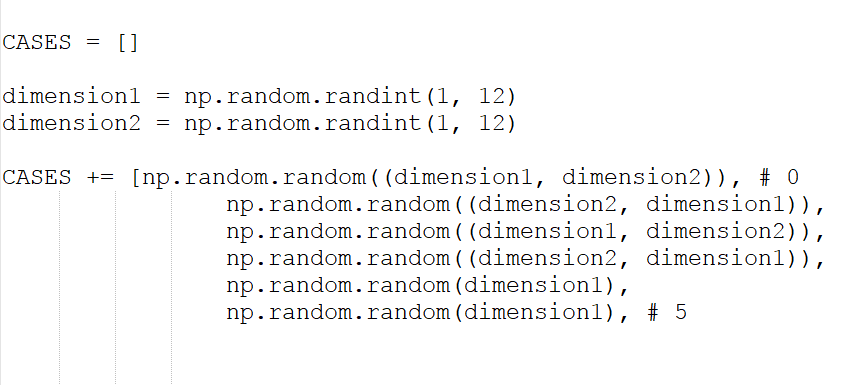
\includegraphics[width=0.6\textwidth]{snippets/multi_dot/1CASES.PNG}
	\includegraphics[width=0.6\textwidth]{snippets/multi_dot/2.png}
	\includegraphics[width=0.6\textwidth]{snippets/multi_dot/3.png}
	\includegraphics[width=0.5\textwidth]{snippets/multi_dot/4.png}

\end{figure}

\subsection{test\_matrix\_rank}	
\begin{figure}[h]
	\centering
	\includegraphics[width=0.70\textwidth]{snippets/rank/1.png}
\end{figure}

\subsection{test\_matrix\_determinant}	
\begin{figure}[h]
	\centering
	\includegraphics[width=0.70\textwidth]{snippets/Det/1.png}
\end{figure}

\subsection{test\_datatypes}	
\begin{figure}[h]
	\centering
	\includegraphics[width=0.70\textwidth]{snippets/datatypes/2.png}
	\includegraphics[width=0.70\textwidth]{snippets/datatypes/3.png}
	\includegraphics[width=0.70\textwidth]{snippets/datatypes/4.png}
\end{figure}

\newpage	
\end{document}
=======





<!DOCTYPE html>
<html lang="en">
  <head>
    <meta charset="utf-8">
  <link rel="dns-prefetch" href="https://assets-cdn.github.com">
  <link rel="dns-prefetch" href="https://avatars0.githubusercontent.com">
  <link rel="dns-prefetch" href="https://avatars1.githubusercontent.com">
  <link rel="dns-prefetch" href="https://avatars2.githubusercontent.com">
  <link rel="dns-prefetch" href="https://avatars3.githubusercontent.com">
  <link rel="dns-prefetch" href="https://github-cloud.s3.amazonaws.com">
  <link rel="dns-prefetch" href="https://user-images.githubusercontent.com/">



  <link crossorigin="anonymous" href="https://assets-cdn.github.com/assets/frameworks-f27d807afb610bf126cbfb9ce429438a328e012239e5a77fc8152b794553dfc0.css" integrity="sha256-8n2AevthC/Emy/uc5ClDijKOASI55ad/yBUreUVT38A=" media="all" rel="stylesheet" />
  <link crossorigin="anonymous" href="https://assets-cdn.github.com/assets/github-1babc1bd6327bf889358e4d39d284da9b84127f3154b925b3f2804d77dc80aea.css" integrity="sha256-G6vBvWMnv4iTWOTTnShNqbhBJ/MVS5JbPygE133ICuo=" media="all" rel="stylesheet" />
  
  
  
  

  <meta name="viewport" content="width=device-width">
  
  <title>STpythontest/testdiary.tex at johansBranch · lavapuppet/STpythontest</title>
  <link rel="search" type="application/opensearchdescription+xml" href="/opensearch.xml" title="GitHub">
  <link rel="fluid-icon" href="https://github.com/fluidicon.png" title="GitHub">
  <meta property="fb:app_id" content="1401488693436528">

    
    <meta content="https://avatars2.githubusercontent.com/u/22473042?s=400&amp;v=4" property="og:image" /><meta content="GitHub" property="og:site_name" /><meta content="object" property="og:type" /><meta content="lavapuppet/STpythontest" property="og:title" /><meta content="https://github.com/lavapuppet/STpythontest" property="og:url" /><meta content="STpythontest - Black box tests for numpy.linalg" property="og:description" />

  <link rel="assets" href="https://assets-cdn.github.com/">
  <link rel="web-socket" href="wss://live.github.com/_sockets/VjI6MjM3NDA2ODU1OjYxYWZhYWRjYThmZTNiZjZhYjI2OTc1ZmY4YzNlZDZjNDIyMGMwZGZlNGU5ZTk2ODZkOGQ2OTE3Njk2NzBiNmU=--7811172fd5f4e4561deafbc692a8913703c04ec9">
  <meta name="pjax-timeout" content="1000">
  <link rel="sudo-modal" href="/sessions/sudo_modal">
  <meta name="request-id" content="65D8:7671:3D066B6:62C6417:5A53AA84" data-pjax-transient>
  

  <meta name="selected-link" value="repo_source" data-pjax-transient>

    <meta name="google-site-verification" content="KT5gs8h0wvaagLKAVWq8bbeNwnZZK1r1XQysX3xurLU">
  <meta name="google-site-verification" content="ZzhVyEFwb7w3e0-uOTltm8Jsck2F5StVihD0exw2fsA">
  <meta name="google-site-verification" content="GXs5KoUUkNCoaAZn7wPN-t01Pywp9M3sEjnt_3_ZWPc">
    <meta name="google-analytics" content="UA-3769691-2">

<meta content="collector.githubapp.com" name="octolytics-host" /><meta content="github" name="octolytics-app-id" /><meta content="https://collector.githubapp.com/github-external/browser_event" name="octolytics-event-url" /><meta content="65D8:7671:3D066B6:62C6417:5A53AA84" name="octolytics-dimension-request_id" /><meta content="iad" name="octolytics-dimension-region_edge" /><meta content="iad" name="octolytics-dimension-region_render" /><meta content="22473042" name="octolytics-actor-id" /><meta content="lavapuppet" name="octolytics-actor-login" /><meta content="9c28c88bcf82558a52855bd55ba82e2279ae90d52ceb3e486e9a6c76aaea7031" name="octolytics-actor-hash" />
<meta content="/&lt;user-name&gt;/&lt;repo-name&gt;/blob/show" data-pjax-transient="true" name="analytics-location" />




  <meta class="js-ga-set" name="dimension1" content="Logged In">


  

      <meta name="hostname" content="github.com">
  <meta name="user-login" content="lavapuppet">

      <meta name="expected-hostname" content="github.com">
    <meta name="js-proxy-site-detection-payload" content="ZmE4ZWZmZTg3MzRhODhiN2FjMGM5NmEwM2NmOWIzYTEzYmI5OTQxNjFiNGUxYjM3YWM4MzFkYTkzZGJiZjEzY3x7InJlbW90ZV9hZGRyZXNzIjoiMTg1LjExMy45OS4xNTIiLCJyZXF1ZXN0X2lkIjoiNjVEODo3NjcxOjNEMDY2QjY6NjJDNjQxNzo1QTUzQUE4NCIsInRpbWVzdGFtcCI6MTUxNTQzMjU4OCwiaG9zdCI6ImdpdGh1Yi5jb20ifQ==">

    <meta name="enabled-features" content="UNIVERSE_BANNER,FREE_TRIALS">

  <meta name="html-safe-nonce" content="7e0245c38f1ae40c1a772eaf6480eeed8502b394">

  <meta http-equiv="x-pjax-version" content="f02a8298c17541294e5dad2f8f44600a">
  

      <link href="https://github.com/lavapuppet/STpythontest/commits/johansBranch.atom" rel="alternate" title="Recent Commits to STpythontest:johansBranch" type="application/atom+xml">

  <meta name="description" content="STpythontest - Black box tests for numpy.linalg">
  <meta name="go-import" content="github.com/lavapuppet/STpythontest git https://github.com/lavapuppet/STpythontest.git">

  <meta content="22473042" name="octolytics-dimension-user_id" /><meta content="lavapuppet" name="octolytics-dimension-user_login" /><meta content="111672375" name="octolytics-dimension-repository_id" /><meta content="lavapuppet/STpythontest" name="octolytics-dimension-repository_nwo" /><meta content="true" name="octolytics-dimension-repository_public" /><meta content="false" name="octolytics-dimension-repository_is_fork" /><meta content="111672375" name="octolytics-dimension-repository_network_root_id" /><meta content="lavapuppet/STpythontest" name="octolytics-dimension-repository_network_root_nwo" /><meta content="true" name="octolytics-dimension-repository_explore_github_marketplace_ci_cta_shown" />


    <link rel="canonical" href="https://github.com/lavapuppet/STpythontest/blob/johansBranch/Diary/testdiary.tex" data-pjax-transient>


  <meta name="browser-stats-url" content="https://api.github.com/_private/browser/stats">

  <meta name="browser-errors-url" content="https://api.github.com/_private/browser/errors">

  <link rel="mask-icon" href="https://assets-cdn.github.com/pinned-octocat.svg" color="#000000">
  <link rel="icon" type="image/x-icon" class="js-site-favicon" href="https://assets-cdn.github.com/favicon.ico">

<meta name="theme-color" content="#1e2327">


  <meta name="u2f-support" content="true">

  </head>

  <body class="logged-in env-production page-blob">
    

  <div class="position-relative js-header-wrapper ">
    <a href="#start-of-content" tabindex="1" class="bg-black text-white p-3 show-on-focus js-skip-to-content">Skip to content</a>
    <div id="js-pjax-loader-bar" class="pjax-loader-bar"><div class="progress"></div></div>

    
    
    
      



        
<header class="Header  f5" role="banner">
  <div class="d-flex px-3 flex-justify-between container-lg">
    <div class="d-flex flex-justify-between">
      <a class="header-logo-invertocat" href="https://github.com/" data-hotkey="g d" aria-label="Homepage" data-ga-click="Header, go to dashboard, icon:logo">
  <svg aria-hidden="true" class="octicon octicon-mark-github" height="32" version="1.1" viewBox="0 0 16 16" width="32"><path fill-rule="evenodd" d="M8 0C3.58 0 0 3.58 0 8c0 3.54 2.29 6.53 5.47 7.59.4.07.55-.17.55-.38 0-.19-.01-.82-.01-1.49-2.01.37-2.53-.49-2.69-.94-.09-.23-.48-.94-.82-1.13-.28-.15-.68-.52-.01-.53.63-.01 1.08.58 1.23.82.72 1.21 1.87.87 2.33.66.07-.52.28-.87.51-1.07-1.78-.2-3.64-.89-3.64-3.95 0-.87.31-1.59.82-2.15-.08-.2-.36-1.02.08-2.12 0 0 .67-.21 2.2.82.64-.18 1.32-.27 2-.27.68 0 1.36.09 2 .27 1.53-1.04 2.2-.82 2.2-.82.44 1.1.16 1.92.08 2.12.51.56.82 1.27.82 2.15 0 3.07-1.87 3.75-3.65 3.95.29.25.54.73.54 1.48 0 1.07-.01 1.93-.01 2.2 0 .21.15.46.55.38A8.013 8.013 0 0 0 16 8c0-4.42-3.58-8-8-8z"/></svg>
</a>


    </div>

    <div class="HeaderMenu d-flex flex-justify-between flex-auto">
      <div class="d-flex">
            <div class="">
              <div class="header-search scoped-search site-scoped-search js-site-search" role="search">
  <!-- '"` --><!-- </textarea></xmp> --></option></form><form accept-charset="UTF-8" action="/lavapuppet/STpythontest/search" class="js-site-search-form" data-scoped-search-url="/lavapuppet/STpythontest/search" data-unscoped-search-url="/search" method="get"><div style="margin:0;padding:0;display:inline"><input name="utf8" type="hidden" value="&#x2713;" /></div>
    <label class="form-control header-search-wrapper js-chromeless-input-container">
        <a href="/lavapuppet/STpythontest/blob/johansBranch/Diary/testdiary.tex" class="header-search-scope no-underline">This repository</a>
      <input type="text"
        class="form-control header-search-input js-site-search-focus js-site-search-field is-clearable"
        data-hotkey="s"
        name="q"
        value=""
        placeholder="Search"
        aria-label="Search this repository"
        data-unscoped-placeholder="Search GitHub"
        data-scoped-placeholder="Search"
        autocapitalize="off">
        <input type="hidden" class="js-site-search-type-field" name="type" >
    </label>
</form></div>

            </div>

          <ul class="d-flex pl-2 flex-items-center text-bold list-style-none" role="navigation">
            <li>
              <a href="/pulls" aria-label="Pull requests you created" class="js-selected-navigation-item HeaderNavlink px-2" data-ga-click="Header, click, Nav menu - item:pulls context:user" data-hotkey="g p" data-selected-links="/pulls /pulls/assigned /pulls/mentioned /pulls">
                Pull requests
</a>            </li>
            <li>
              <a href="/issues" aria-label="Issues you created" class="js-selected-navigation-item HeaderNavlink px-2" data-ga-click="Header, click, Nav menu - item:issues context:user" data-hotkey="g i" data-selected-links="/issues /issues/assigned /issues/mentioned /issues">
                Issues
</a>            </li>
                <li>
                  <a href="/marketplace" class="js-selected-navigation-item HeaderNavlink px-2" data-ga-click="Header, click, Nav menu - item:marketplace context:user" data-selected-links=" /marketplace">
                    Marketplace
</a>                </li>
            <li>
              <a href="/explore" class="js-selected-navigation-item HeaderNavlink px-2" data-ga-click="Header, click, Nav menu - item:explore" data-selected-links="/explore /trending /trending/developers /integrations /integrations/feature/code /integrations/feature/collaborate /integrations/feature/ship showcases showcases_search showcases_landing /explore">
                Explore
</a>            </li>
          </ul>
      </div>

      <div class="d-flex">
        
<ul class="user-nav d-flex flex-items-center list-style-none" id="user-links">
  <li class="dropdown js-menu-container">
    <span class="d-inline-block  px-2">
      

    </span>
  </li>

  <li class="dropdown js-menu-container">
    <details class="dropdown-details details-reset js-dropdown-details d-flex px-2 flex-items-center">
      <summary class="HeaderNavlink"
         aria-label="Create new…"
         data-ga-click="Header, create new, icon:add">
        <svg aria-hidden="true" class="octicon octicon-plus float-left mr-1 mt-1" height="16" version="1.1" viewBox="0 0 12 16" width="12"><path fill-rule="evenodd" d="M12 9H7v5H5V9H0V7h5V2h2v5h5z"/></svg>
        <span class="dropdown-caret mt-1"></span>
      </summary>

      <ul class="dropdown-menu dropdown-menu-sw">
        
<a class="dropdown-item" href="/new" data-ga-click="Header, create new repository">
  New repository
</a>

  <a class="dropdown-item" href="/new/import" data-ga-click="Header, import a repository">
    Import repository
  </a>

<a class="dropdown-item" href="https://gist.github.com/" data-ga-click="Header, create new gist">
  New gist
</a>

  <a class="dropdown-item" href="/organizations/new" data-ga-click="Header, create new organization">
    New organization
  </a>



  <div class="dropdown-divider"></div>
  <div class="dropdown-header">
    <span title="lavapuppet/STpythontest">This repository</span>
  </div>
    <a class="dropdown-item" href="/lavapuppet/STpythontest/issues/new" data-ga-click="Header, create new issue">
      New issue
    </a>

      </ul>
    </details>
  </li>

  <li class="dropdown js-menu-container">

    <details class="dropdown-details details-reset js-dropdown-details d-flex pl-2 flex-items-center">
      <summary class="HeaderNavlink name mt-1"
        aria-label="View profile and more"
        data-ga-click="Header, show menu, icon:avatar">
        <img alt="@lavapuppet" class="avatar float-left mr-1" src="https://avatars3.githubusercontent.com/u/22473042?s=40&amp;v=4" height="20" width="20">
        <span class="dropdown-caret"></span>
      </summary>

      <ul class="dropdown-menu dropdown-menu-sw">
        <li class="dropdown-header header-nav-current-user css-truncate">
          Signed in as <strong class="css-truncate-target">lavapuppet</strong>
        </li>

        <li class="dropdown-divider"></li>

        <li><a class="dropdown-item" href="/lavapuppet" data-ga-click="Header, go to profile, text:your profile">
          Your profile
        </a></li>
        <li><a class="dropdown-item" href="/lavapuppet?tab=stars" data-ga-click="Header, go to starred repos, text:your stars">
          Your stars
        </a></li>
          <li><a class="dropdown-item" href="https://gist.github.com/" data-ga-click="Header, your gists, text:your gists">Your Gists</a></li>

        <li class="dropdown-divider"></li>

        <li><a class="dropdown-item" href="https://help.github.com" data-ga-click="Header, go to help, text:help">
          Help
        </a></li>

        <li><a class="dropdown-item" href="/settings/profile" data-ga-click="Header, go to settings, icon:settings">
          Settings
        </a></li>

        <li><!-- '"` --><!-- </textarea></xmp> --></option></form><form accept-charset="UTF-8" action="/logout" class="logout-form" method="post"><div style="margin:0;padding:0;display:inline"><input name="utf8" type="hidden" value="&#x2713;" /><input name="authenticity_token" type="hidden" value="OExuw/GVkC+c3jiASZywPwj26kDg0XrEisEhc7ZrEv/OXodVLhl6inw+IGOtoVqnj0paUWyiLyDNYdo7SU8upA==" /></div>
          <button type="submit" class="dropdown-item dropdown-signout" data-ga-click="Header, sign out, icon:logout">
            Sign out
          </button>
        </form></li>
      </ul>
    </details>
  </li>
</ul>


        <!-- '"` --><!-- </textarea></xmp> --></option></form><form accept-charset="UTF-8" action="/logout" class="sr-only right-0" method="post"><div style="margin:0;padding:0;display:inline"><input name="utf8" type="hidden" value="&#x2713;" /><input name="authenticity_token" type="hidden" value="l3j0qkLHR6JZggRM2K9yYPYTeqrR05KseHckAl5DHk9hah08nUutB7liHK88kpj4ca/Ku12gx0g/199KoWciFA==" /></div>
          <button type="submit" class="dropdown-item dropdown-signout" data-ga-click="Header, sign out, icon:logout">
            Sign out
          </button>
</form>      </div>
    </div>
  </div>
</header>

      

  </div>

  <div id="start-of-content" class="show-on-focus"></div>

    <div id="js-flash-container">
</div>



  <div role="main" >
        <div itemscope itemtype="http://schema.org/SoftwareSourceCode" class="">
    <div id="js-repo-pjax-container" data-pjax-container >
      






  <div class="pagehead repohead instapaper_ignore readability-menu experiment-repo-nav  ">
    <div class="repohead-details-container clearfix container">

      <ul class="pagehead-actions">
  <li>
        <!-- '"` --><!-- </textarea></xmp> --></option></form><form accept-charset="UTF-8" action="/notifications/subscribe" class="js-social-container" data-autosubmit="true" data-remote="true" method="post"><div style="margin:0;padding:0;display:inline"><input name="utf8" type="hidden" value="&#x2713;" /><input name="authenticity_token" type="hidden" value="Jm2ZXsLKVElPSL1ih1JC91lMJJIF8D4lkwgEWtJfxfx+eXLch45MJHYbV6PInSDT2P0+oCxot/qb0QbZgWLp1g==" /></div>      <input class="form-control" id="repository_id" name="repository_id" type="hidden" value="111672375" />

        <div class="select-menu js-menu-container js-select-menu">
          <a href="/lavapuppet/STpythontest/subscription"
            class="btn btn-sm btn-with-count select-menu-button js-menu-target"
            role="button"
            aria-haspopup="true"
            aria-expanded="false"
            aria-label="Toggle repository notifications menu"
            data-ga-click="Repository, click Watch settings, action:blob#show">
            <span class="js-select-button">
                <svg aria-hidden="true" class="octicon octicon-eye" height="16" version="1.1" viewBox="0 0 16 16" width="16"><path fill-rule="evenodd" d="M8.06 2C3 2 0 8 0 8s3 6 8.06 6C13 14 16 8 16 8s-3-6-7.94-6zM8 12c-2.2 0-4-1.78-4-4 0-2.2 1.8-4 4-4 2.22 0 4 1.8 4 4 0 2.22-1.78 4-4 4zm2-4c0 1.11-.89 2-2 2-1.11 0-2-.89-2-2 0-1.11.89-2 2-2 1.11 0 2 .89 2 2z"/></svg>
                Watch
            </span>
          </a>
          <a class="social-count js-social-count"
            href="/lavapuppet/STpythontest/watchers"
            aria-label="0 users are watching this repository">
            0
          </a>

        <div class="select-menu-modal-holder">
          <div class="select-menu-modal subscription-menu-modal js-menu-content">
            <div class="select-menu-header js-navigation-enable" tabindex="-1">
              <svg aria-label="Close" class="octicon octicon-x js-menu-close" height="16" role="img" version="1.1" viewBox="0 0 12 16" width="12"><path fill-rule="evenodd" d="M7.48 8l3.75 3.75-1.48 1.48L6 9.48l-3.75 3.75-1.48-1.48L4.52 8 .77 4.25l1.48-1.48L6 6.52l3.75-3.75 1.48 1.48z"/></svg>
              <span class="select-menu-title">Notifications</span>
            </div>

              <div class="select-menu-list js-navigation-container" role="menu">

                <div class="select-menu-item js-navigation-item selected" role="menuitem" tabindex="0">
                  <svg aria-hidden="true" class="octicon octicon-check select-menu-item-icon" height="16" version="1.1" viewBox="0 0 12 16" width="12"><path fill-rule="evenodd" d="M12 5l-8 8-4-4 1.5-1.5L4 10l6.5-6.5z"/></svg>
                  <div class="select-menu-item-text">
                    <input checked="checked" id="do_included" name="do" type="radio" value="included" />
                    <span class="select-menu-item-heading">Not watching</span>
                    <span class="description">Be notified when participating or @mentioned.</span>
                    <span class="js-select-button-text hidden-select-button-text">
                      <svg aria-hidden="true" class="octicon octicon-eye" height="16" version="1.1" viewBox="0 0 16 16" width="16"><path fill-rule="evenodd" d="M8.06 2C3 2 0 8 0 8s3 6 8.06 6C13 14 16 8 16 8s-3-6-7.94-6zM8 12c-2.2 0-4-1.78-4-4 0-2.2 1.8-4 4-4 2.22 0 4 1.8 4 4 0 2.22-1.78 4-4 4zm2-4c0 1.11-.89 2-2 2-1.11 0-2-.89-2-2 0-1.11.89-2 2-2 1.11 0 2 .89 2 2z"/></svg>
                      Watch
                    </span>
                  </div>
                </div>

                <div class="select-menu-item js-navigation-item " role="menuitem" tabindex="0">
                  <svg aria-hidden="true" class="octicon octicon-check select-menu-item-icon" height="16" version="1.1" viewBox="0 0 12 16" width="12"><path fill-rule="evenodd" d="M12 5l-8 8-4-4 1.5-1.5L4 10l6.5-6.5z"/></svg>
                  <div class="select-menu-item-text">
                    <input id="do_subscribed" name="do" type="radio" value="subscribed" />
                    <span class="select-menu-item-heading">Watching</span>
                    <span class="description">Be notified of all conversations.</span>
                    <span class="js-select-button-text hidden-select-button-text">
                      <svg aria-hidden="true" class="octicon octicon-eye" height="16" version="1.1" viewBox="0 0 16 16" width="16"><path fill-rule="evenodd" d="M8.06 2C3 2 0 8 0 8s3 6 8.06 6C13 14 16 8 16 8s-3-6-7.94-6zM8 12c-2.2 0-4-1.78-4-4 0-2.2 1.8-4 4-4 2.22 0 4 1.8 4 4 0 2.22-1.78 4-4 4zm2-4c0 1.11-.89 2-2 2-1.11 0-2-.89-2-2 0-1.11.89-2 2-2 1.11 0 2 .89 2 2z"/></svg>
                        Unwatch
                    </span>
                  </div>
                </div>

                <div class="select-menu-item js-navigation-item " role="menuitem" tabindex="0">
                  <svg aria-hidden="true" class="octicon octicon-check select-menu-item-icon" height="16" version="1.1" viewBox="0 0 12 16" width="12"><path fill-rule="evenodd" d="M12 5l-8 8-4-4 1.5-1.5L4 10l6.5-6.5z"/></svg>
                  <div class="select-menu-item-text">
                    <input id="do_ignore" name="do" type="radio" value="ignore" />
                    <span class="select-menu-item-heading">Ignoring</span>
                    <span class="description">Never be notified.</span>
                    <span class="js-select-button-text hidden-select-button-text">
                      <svg aria-hidden="true" class="octicon octicon-mute" height="16" version="1.1" viewBox="0 0 16 16" width="16"><path fill-rule="evenodd" d="M8 2.81v10.38c0 .67-.81 1-1.28.53L3 10H1c-.55 0-1-.45-1-1V7c0-.55.45-1 1-1h2l3.72-3.72C7.19 1.81 8 2.14 8 2.81zm7.53 3.22l-1.06-1.06-1.97 1.97-1.97-1.97-1.06 1.06L11.44 8 9.47 9.97l1.06 1.06 1.97-1.97 1.97 1.97 1.06-1.06L13.56 8l1.97-1.97z"/></svg>
                        Stop ignoring
                    </span>
                  </div>
                </div>

              </div>

            </div>
          </div>
        </div>
</form>
  </li>

  <li>
    
  <div class="js-toggler-container js-social-container starring-container ">
    <!-- '"` --><!-- </textarea></xmp> --></option></form><form accept-charset="UTF-8" action="/lavapuppet/STpythontest/unstar" class="starred js-social-form" method="post"><div style="margin:0;padding:0;display:inline"><input name="utf8" type="hidden" value="&#x2713;" /><input name="authenticity_token" type="hidden" value="17n3iop0nZmepiYS21DcPAhBP38PVae6OeiD3PmddGMl2CWjz1mjuqIBEegQ1FWxapElehQoCGstZCS2NCEtOg==" /></div>
      <input type="hidden" name="context" value="repository"></input>
      <button
        type="submit"
        class="btn btn-sm btn-with-count js-toggler-target"
        aria-label="Unstar this repository" title="Unstar lavapuppet/STpythontest"
        data-ga-click="Repository, click unstar button, action:blob#show; text:Unstar">
        <svg aria-hidden="true" class="octicon octicon-star" height="16" version="1.1" viewBox="0 0 14 16" width="14"><path fill-rule="evenodd" d="M14 6l-4.9-.64L7 1 4.9 5.36 0 6l3.6 3.26L2.67 14 7 11.67 11.33 14l-.93-4.74z"/></svg>
        Unstar
      </button>
        <a class="social-count js-social-count" href="/lavapuppet/STpythontest/stargazers"
           aria-label="0 users starred this repository">
          0
        </a>
</form>
    <!-- '"` --><!-- </textarea></xmp> --></option></form><form accept-charset="UTF-8" action="/lavapuppet/STpythontest/star" class="unstarred js-social-form" method="post"><div style="margin:0;padding:0;display:inline"><input name="utf8" type="hidden" value="&#x2713;" /><input name="authenticity_token" type="hidden" value="42YrQ/fqA7ffM/IOBkzpRB/92aYbeI9nXzMGpuCcFO3IkHXRS17i2UMTANO4gOU/mj6WxQU6CtSmkBQXkV/aCA==" /></div>
      <input type="hidden" name="context" value="repository"></input>
      <button
        type="submit"
        class="btn btn-sm btn-with-count js-toggler-target"
        aria-label="Star this repository" title="Star lavapuppet/STpythontest"
        data-ga-click="Repository, click star button, action:blob#show; text:Star">
        <svg aria-hidden="true" class="octicon octicon-star" height="16" version="1.1" viewBox="0 0 14 16" width="14"><path fill-rule="evenodd" d="M14 6l-4.9-.64L7 1 4.9 5.36 0 6l3.6 3.26L2.67 14 7 11.67 11.33 14l-.93-4.74z"/></svg>
        Star
      </button>
        <a class="social-count js-social-count" href="/lavapuppet/STpythontest/stargazers"
           aria-label="0 users starred this repository">
          0
        </a>
</form>  </div>

  </li>

  <li>
          <!-- '"` --><!-- </textarea></xmp> --></option></form><form accept-charset="UTF-8" action="/lavapuppet/STpythontest/fork" class="btn-with-count" method="post"><div style="margin:0;padding:0;display:inline"><input name="utf8" type="hidden" value="&#x2713;" /><input name="authenticity_token" type="hidden" value="nO+Du+knpeNkkyr5w1SmI0fFbACXnvwmMKiOdcilAqG/AnTQB5iOjcKoBpoDBpTdEiZIb2z2YYDrs+d+8qwu7A==" /></div>
            <button
                type="submit"
                class="btn btn-sm btn-with-count"
                data-ga-click="Repository, show fork modal, action:blob#show; text:Fork"
                title="Fork your own copy of lavapuppet/STpythontest to your account"
                aria-label="Fork your own copy of lavapuppet/STpythontest to your account">
              <svg aria-hidden="true" class="octicon octicon-repo-forked" height="16" version="1.1" viewBox="0 0 10 16" width="10"><path fill-rule="evenodd" d="M8 1a1.993 1.993 0 0 0-1 3.72V6L5 8 3 6V4.72A1.993 1.993 0 0 0 2 1a1.993 1.993 0 0 0-1 3.72V6.5l3 3v1.78A1.993 1.993 0 0 0 5 15a1.993 1.993 0 0 0 1-3.72V9.5l3-3V4.72A1.993 1.993 0 0 0 8 1zM2 4.2C1.34 4.2.8 3.65.8 3c0-.65.55-1.2 1.2-1.2.65 0 1.2.55 1.2 1.2 0 .65-.55 1.2-1.2 1.2zm3 10c-.66 0-1.2-.55-1.2-1.2 0-.65.55-1.2 1.2-1.2.65 0 1.2.55 1.2 1.2 0 .65-.55 1.2-1.2 1.2zm3-10c-.66 0-1.2-.55-1.2-1.2 0-.65.55-1.2 1.2-1.2.65 0 1.2.55 1.2 1.2 0 .65-.55 1.2-1.2 1.2z"/></svg>
              Fork
            </button>
</form>
    <a href="/lavapuppet/STpythontest/network" class="social-count"
       aria-label="1 user forked this repository">
      1
    </a>
  </li>
</ul>

      <h1 class="public ">
  <svg aria-hidden="true" class="octicon octicon-repo" height="16" version="1.1" viewBox="0 0 12 16" width="12"><path fill-rule="evenodd" d="M4 9H3V8h1v1zm0-3H3v1h1V6zm0-2H3v1h1V4zm0-2H3v1h1V2zm8-1v12c0 .55-.45 1-1 1H6v2l-1.5-1.5L3 16v-2H1c-.55 0-1-.45-1-1V1c0-.55.45-1 1-1h10c.55 0 1 .45 1 1zm-1 10H1v2h2v-1h3v1h5v-2zm0-10H2v9h9V1z"/></svg>
  <span class="author" itemprop="author"><a href="/lavapuppet" class="url fn" rel="author">lavapuppet</a></span><!--
--><span class="path-divider">/</span><!--
--><strong itemprop="name"><a href="/lavapuppet/STpythontest" data-pjax="#js-repo-pjax-container">STpythontest</a></strong>

</h1>

    </div>
    
<nav class="reponav js-repo-nav js-sidenav-container-pjax container"
     itemscope
     itemtype="http://schema.org/BreadcrumbList"
     role="navigation"
     data-pjax="#js-repo-pjax-container">

  <span itemscope itemtype="http://schema.org/ListItem" itemprop="itemListElement">
    <a href="/lavapuppet/STpythontest/tree/johansBranch" class="js-selected-navigation-item selected reponav-item" data-hotkey="g c" data-selected-links="repo_source repo_downloads repo_commits repo_releases repo_tags repo_branches repo_packages /lavapuppet/STpythontest/tree/johansBranch" itemprop="url">
      <svg aria-hidden="true" class="octicon octicon-code" height="16" version="1.1" viewBox="0 0 14 16" width="14"><path fill-rule="evenodd" d="M9.5 3L8 4.5 11.5 8 8 11.5 9.5 13 14 8 9.5 3zm-5 0L0 8l4.5 5L6 11.5 2.5 8 6 4.5 4.5 3z"/></svg>
      <span itemprop="name">Code</span>
      <meta itemprop="position" content="1">
</a>  </span>

    <span itemscope itemtype="http://schema.org/ListItem" itemprop="itemListElement">
      <a href="/lavapuppet/STpythontest/issues" class="js-selected-navigation-item reponav-item" data-hotkey="g i" data-selected-links="repo_issues repo_labels repo_milestones /lavapuppet/STpythontest/issues" itemprop="url">
        <svg aria-hidden="true" class="octicon octicon-issue-opened" height="16" version="1.1" viewBox="0 0 14 16" width="14"><path fill-rule="evenodd" d="M7 2.3c3.14 0 5.7 2.56 5.7 5.7s-2.56 5.7-5.7 5.7A5.71 5.71 0 0 1 1.3 8c0-3.14 2.56-5.7 5.7-5.7zM7 1C3.14 1 0 4.14 0 8s3.14 7 7 7 7-3.14 7-7-3.14-7-7-7zm1 3H6v5h2V4zm0 6H6v2h2v-2z"/></svg>
        <span itemprop="name">Issues</span>
        <span class="Counter">0</span>
        <meta itemprop="position" content="2">
</a>    </span>

  <span itemscope itemtype="http://schema.org/ListItem" itemprop="itemListElement">
    <a href="/lavapuppet/STpythontest/pulls" class="js-selected-navigation-item reponav-item" data-hotkey="g p" data-selected-links="repo_pulls /lavapuppet/STpythontest/pulls" itemprop="url">
      <svg aria-hidden="true" class="octicon octicon-git-pull-request" height="16" version="1.1" viewBox="0 0 12 16" width="12"><path fill-rule="evenodd" d="M11 11.28V5c-.03-.78-.34-1.47-.94-2.06C9.46 2.35 8.78 2.03 8 2H7V0L4 3l3 3V4h1c.27.02.48.11.69.31.21.2.3.42.31.69v6.28A1.993 1.993 0 0 0 10 15a1.993 1.993 0 0 0 1-3.72zm-1 2.92c-.66 0-1.2-.55-1.2-1.2 0-.65.55-1.2 1.2-1.2.65 0 1.2.55 1.2 1.2 0 .65-.55 1.2-1.2 1.2zM4 3c0-1.11-.89-2-2-2a1.993 1.993 0 0 0-1 3.72v6.56A1.993 1.993 0 0 0 2 15a1.993 1.993 0 0 0 1-3.72V4.72c.59-.34 1-.98 1-1.72zm-.8 10c0 .66-.55 1.2-1.2 1.2-.65 0-1.2-.55-1.2-1.2 0-.65.55-1.2 1.2-1.2.65 0 1.2.55 1.2 1.2zM2 4.2C1.34 4.2.8 3.65.8 3c0-.65.55-1.2 1.2-1.2.65 0 1.2.55 1.2 1.2 0 .65-.55 1.2-1.2 1.2z"/></svg>
      <span itemprop="name">Pull requests</span>
      <span class="Counter">0</span>
      <meta itemprop="position" content="3">
</a>  </span>

    <a href="/lavapuppet/STpythontest/projects" class="js-selected-navigation-item reponav-item" data-hotkey="g b" data-selected-links="repo_projects new_repo_project repo_project /lavapuppet/STpythontest/projects">
      <svg aria-hidden="true" class="octicon octicon-project" height="16" version="1.1" viewBox="0 0 15 16" width="15"><path fill-rule="evenodd" d="M10 12h3V2h-3v10zm-4-2h3V2H6v8zm-4 4h3V2H2v12zm-1 1h13V1H1v14zM14 0H1a1 1 0 0 0-1 1v14a1 1 0 0 0 1 1h13a1 1 0 0 0 1-1V1a1 1 0 0 0-1-1z"/></svg>
      Projects
      <span class="Counter" >0</span>
</a>
    <a href="/lavapuppet/STpythontest/wiki" class="js-selected-navigation-item reponav-item" data-hotkey="g w" data-selected-links="repo_wiki /lavapuppet/STpythontest/wiki">
      <svg aria-hidden="true" class="octicon octicon-book" height="16" version="1.1" viewBox="0 0 16 16" width="16"><path fill-rule="evenodd" d="M3 5h4v1H3V5zm0 3h4V7H3v1zm0 2h4V9H3v1zm11-5h-4v1h4V5zm0 2h-4v1h4V7zm0 2h-4v1h4V9zm2-6v9c0 .55-.45 1-1 1H9.5l-1 1-1-1H2c-.55 0-1-.45-1-1V3c0-.55.45-1 1-1h5.5l1 1 1-1H15c.55 0 1 .45 1 1zm-8 .5L7.5 3H2v9h6V3.5zm7-.5H9.5l-.5.5V12h6V3z"/></svg>
      Wiki
</a>

  <a href="/lavapuppet/STpythontest/pulse" class="js-selected-navigation-item reponav-item" data-selected-links="repo_graphs repo_contributors dependency_graph pulse /lavapuppet/STpythontest/pulse">
    <svg aria-hidden="true" class="octicon octicon-graph" height="16" version="1.1" viewBox="0 0 16 16" width="16"><path fill-rule="evenodd" d="M16 14v1H0V0h1v14h15zM5 13H3V8h2v5zm4 0H7V3h2v10zm4 0h-2V6h2v7z"/></svg>
    Insights
</a>
    <a href="/lavapuppet/STpythontest/settings" class="js-selected-navigation-item reponav-item" data-selected-links="repo_settings repo_branch_settings hooks integration_installations repo_keys_settings /lavapuppet/STpythontest/settings">
      <svg aria-hidden="true" class="octicon octicon-gear" height="16" version="1.1" viewBox="0 0 14 16" width="14"><path fill-rule="evenodd" d="M14 8.77v-1.6l-1.94-.64-.45-1.09.88-1.84-1.13-1.13-1.81.91-1.09-.45-.69-1.92h-1.6l-.63 1.94-1.11.45-1.84-.88-1.13 1.13.91 1.81-.45 1.09L0 7.23v1.59l1.94.64.45 1.09-.88 1.84 1.13 1.13 1.81-.91 1.09.45.69 1.92h1.59l.63-1.94 1.11-.45 1.84.88 1.13-1.13-.92-1.81.47-1.09L14 8.75v.02zM7 11c-1.66 0-3-1.34-3-3s1.34-3 3-3 3 1.34 3 3-1.34 3-3 3z"/></svg>
      Settings
</a>
</nav>


  </div>

<div class="container new-discussion-timeline experiment-repo-nav ">
  <div class="repository-content ">

    
  <a href="/lavapuppet/STpythontest/blob/0710aab0f9273223c28a2f9e4b94e312f5410038/Diary/testdiary.tex" class="d-none js-permalink-shortcut" data-hotkey="y">Permalink</a>

  <!-- blob contrib key: blob_contributors:v21:f84c7f66febdc5870d622a57996d94be -->

  <div class="file-navigation js-zeroclipboard-container">
    
<div class="select-menu branch-select-menu js-menu-container js-select-menu float-left">
  <button class=" btn btn-sm select-menu-button js-menu-target css-truncate" data-hotkey="w"
    
    type="button" aria-label="Switch branches or tags" aria-expanded="false" aria-haspopup="true">
      <i>Branch:</i>
      <span class="js-select-button css-truncate-target">johansBranch</span>
  </button>

  <div class="select-menu-modal-holder js-menu-content js-navigation-container" data-pjax>

    <div class="select-menu-modal">
      <div class="select-menu-header">
        <svg aria-label="Close" class="octicon octicon-x js-menu-close" height="16" role="img" version="1.1" viewBox="0 0 12 16" width="12"><path fill-rule="evenodd" d="M7.48 8l3.75 3.75-1.48 1.48L6 9.48l-3.75 3.75-1.48-1.48L4.52 8 .77 4.25l1.48-1.48L6 6.52l3.75-3.75 1.48 1.48z"/></svg>
        <span class="select-menu-title">Switch branches/tags</span>
      </div>

      <div class="select-menu-filters">
        <div class="select-menu-text-filter">
          <input type="text" aria-label="Find or create a branch…" id="context-commitish-filter-field" class="form-control js-filterable-field js-navigation-enable" placeholder="Find or create a branch…">
        </div>
        <div class="select-menu-tabs">
          <ul>
            <li class="select-menu-tab">
              <a href="#" data-tab-filter="branches" data-filter-placeholder="Find or create a branch…" class="js-select-menu-tab" role="tab">Branches</a>
            </li>
            <li class="select-menu-tab">
              <a href="#" data-tab-filter="tags" data-filter-placeholder="Find a tag…" class="js-select-menu-tab" role="tab">Tags</a>
            </li>
          </ul>
        </div>
      </div>

      <div class="select-menu-list select-menu-tab-bucket js-select-menu-tab-bucket" data-tab-filter="branches" role="menu">

        <div data-filterable-for="context-commitish-filter-field" data-filterable-type="substring">


            <a class="select-menu-item js-navigation-item js-navigation-open "
               href="/lavapuppet/STpythontest/blob/johan/Diary/testdiary.tex"
               data-name="johan"
               data-skip-pjax="true"
               rel="nofollow">
              <svg aria-hidden="true" class="octicon octicon-check select-menu-item-icon" height="16" version="1.1" viewBox="0 0 12 16" width="12"><path fill-rule="evenodd" d="M12 5l-8 8-4-4 1.5-1.5L4 10l6.5-6.5z"/></svg>
              <span class="select-menu-item-text css-truncate-target js-select-menu-filter-text">
                johan
              </span>
            </a>
            <a class="select-menu-item js-navigation-item js-navigation-open selected"
               href="/lavapuppet/STpythontest/blob/johansBranch/Diary/testdiary.tex"
               data-name="johansBranch"
               data-skip-pjax="true"
               rel="nofollow">
              <svg aria-hidden="true" class="octicon octicon-check select-menu-item-icon" height="16" version="1.1" viewBox="0 0 12 16" width="12"><path fill-rule="evenodd" d="M12 5l-8 8-4-4 1.5-1.5L4 10l6.5-6.5z"/></svg>
              <span class="select-menu-item-text css-truncate-target js-select-menu-filter-text">
                johansBranch
              </span>
            </a>
            <a class="select-menu-item js-navigation-item js-navigation-open "
               href="/lavapuppet/STpythontest/blob/master/Diary/testdiary.tex"
               data-name="master"
               data-skip-pjax="true"
               rel="nofollow">
              <svg aria-hidden="true" class="octicon octicon-check select-menu-item-icon" height="16" version="1.1" viewBox="0 0 12 16" width="12"><path fill-rule="evenodd" d="M12 5l-8 8-4-4 1.5-1.5L4 10l6.5-6.5z"/></svg>
              <span class="select-menu-item-text css-truncate-target js-select-menu-filter-text">
                master
              </span>
            </a>
        </div>

          <!-- '"` --><!-- </textarea></xmp> --></option></form><form accept-charset="UTF-8" action="/lavapuppet/STpythontest/branches" class="js-create-branch select-menu-item select-menu-new-item-form js-navigation-item js-new-item-form" method="post"><div style="margin:0;padding:0;display:inline"><input name="utf8" type="hidden" value="&#x2713;" /><input name="authenticity_token" type="hidden" value="AJOROWVfu7OtH8Pcovn4enh7Cms8GkgkGZbtywdjcuZPDA37jX64BWeVzzrP+SbCi9bZYcSVDGqVFoVCpx7cDg==" /></div>
          <svg aria-hidden="true" class="octicon octicon-git-branch select-menu-item-icon" height="16" version="1.1" viewBox="0 0 10 16" width="10"><path fill-rule="evenodd" d="M10 5c0-1.11-.89-2-2-2a1.993 1.993 0 0 0-1 3.72v.3c-.02.52-.23.98-.63 1.38-.4.4-.86.61-1.38.63-.83.02-1.48.16-2 .45V4.72a1.993 1.993 0 0 0-1-3.72C.88 1 0 1.89 0 3a2 2 0 0 0 1 1.72v6.56c-.59.35-1 .99-1 1.72 0 1.11.89 2 2 2 1.11 0 2-.89 2-2 0-.53-.2-1-.53-1.36.09-.06.48-.41.59-.47.25-.11.56-.17.94-.17 1.05-.05 1.95-.45 2.75-1.25S8.95 7.77 9 6.73h-.02C9.59 6.37 10 5.73 10 5zM2 1.8c.66 0 1.2.55 1.2 1.2 0 .65-.55 1.2-1.2 1.2C1.35 4.2.8 3.65.8 3c0-.65.55-1.2 1.2-1.2zm0 12.41c-.66 0-1.2-.55-1.2-1.2 0-.65.55-1.2 1.2-1.2.65 0 1.2.55 1.2 1.2 0 .65-.55 1.2-1.2 1.2zm6-8c-.66 0-1.2-.55-1.2-1.2 0-.65.55-1.2 1.2-1.2.65 0 1.2.55 1.2 1.2 0 .65-.55 1.2-1.2 1.2z"/></svg>
            <div class="select-menu-item-text">
              <span class="select-menu-item-heading">Create branch: <span class="js-new-item-name"></span></span>
              <span class="description">from ‘johansBranch’</span>
            </div>
            <input type="hidden" name="name" id="name" class="js-new-item-value">
            <input type="hidden" name="branch" id="branch" value="johansBranch">
            <input type="hidden" name="path" id="path" value="Diary/testdiary.tex">
</form>
      </div>

      <div class="select-menu-list select-menu-tab-bucket js-select-menu-tab-bucket" data-tab-filter="tags">
        <div data-filterable-for="context-commitish-filter-field" data-filterable-type="substring">


        </div>

        <div class="select-menu-no-results">Nothing to show</div>
      </div>

    </div>
  </div>
</div>

    <div class="BtnGroup float-right">
      <a href="/lavapuppet/STpythontest/find/johansBranch"
            class="js-pjax-capture-input btn btn-sm BtnGroup-item"
            data-pjax
            data-hotkey="t">
        Find file
      </a>
      <button aria-label="Copy file path to clipboard" class="js-zeroclipboard btn btn-sm BtnGroup-item tooltipped tooltipped-s" data-copied-hint="Copied!" type="button">Copy path</button>
    </div>
    <div class="breadcrumb js-zeroclipboard-target">
      <span class="repo-root js-repo-root"><span class="js-path-segment"><a href="/lavapuppet/STpythontest/tree/johansBranch"><span>STpythontest</span></a></span></span><span class="separator">/</span><span class="js-path-segment"><a href="/lavapuppet/STpythontest/tree/johansBranch/Diary"><span>Diary</span></a></span><span class="separator">/</span><strong class="final-path">testdiary.tex</strong>
    </div>
  </div>


  <include-fragment class="commit-tease" src="/lavapuppet/STpythontest/contributors/johansBranch/Diary/testdiary.tex">
    <div>
      Fetching contributors&hellip;
    </div>

    <div class="commit-tease-contributors">
      <img alt="" class="loader-loading float-left" height="16" src="https://assets-cdn.github.com/images/spinners/octocat-spinner-32-EAF2F5.gif" width="16" />
      <span class="loader-error">Cannot retrieve contributors at this time</span>
    </div>
</include-fragment>

  <div class="file">
    <div class="file-header">
  <div class="file-actions">

    <div class="BtnGroup">
      <a href="/lavapuppet/STpythontest/raw/johansBranch/Diary/testdiary.tex" class="btn btn-sm BtnGroup-item" id="raw-url">Raw</a>
        <a href="/lavapuppet/STpythontest/blame/johansBranch/Diary/testdiary.tex" class="btn btn-sm js-update-url-with-hash BtnGroup-item" data-hotkey="b">Blame</a>
      <a href="/lavapuppet/STpythontest/commits/johansBranch/Diary/testdiary.tex" class="btn btn-sm BtnGroup-item" rel="nofollow">History</a>
    </div>


        <!-- '"` --><!-- </textarea></xmp> --></option></form><form accept-charset="UTF-8" action="/lavapuppet/STpythontest/edit/johansBranch/Diary/testdiary.tex" class="inline-form js-update-url-with-hash" method="post"><div style="margin:0;padding:0;display:inline"><input name="utf8" type="hidden" value="&#x2713;" /><input name="authenticity_token" type="hidden" value="v/dz1QN3PE2BDgrqL0W6xKursfpfEk0hOlVsQbOQmZNboPicSmk67JhgM+a+cpgmwHxfrRkyExr92JZnOY9mpA==" /></div>
          <button class="btn-octicon tooltipped tooltipped-nw" type="submit"
            aria-label="Edit this file" data-hotkey="e" data-disable-with>
            <svg aria-hidden="true" class="octicon octicon-pencil" height="16" version="1.1" viewBox="0 0 14 16" width="14"><path fill-rule="evenodd" d="M0 12v3h3l8-8-3-3-8 8zm3 2H1v-2h1v1h1v1zm10.3-9.3L12 6 9 3l1.3-1.3a.996.996 0 0 1 1.41 0l1.59 1.59c.39.39.39 1.02 0 1.41z"/></svg>
          </button>
</form>        <!-- '"` --><!-- </textarea></xmp> --></option></form><form accept-charset="UTF-8" action="/lavapuppet/STpythontest/delete/johansBranch/Diary/testdiary.tex" class="inline-form" method="post"><div style="margin:0;padding:0;display:inline"><input name="utf8" type="hidden" value="&#x2713;" /><input name="authenticity_token" type="hidden" value="xCNfdAdQ7aaN5QeKvvBNcR2mesRzA0Q/1h0bvSGoUiGNF1lWh87Mg4F9d2VP1eJF+xPvb4yzyQtAUEokaNp7jg==" /></div>
          <button class="btn-octicon btn-octicon-danger tooltipped tooltipped-nw" type="submit"
            aria-label="Delete this file" data-disable-with>
            <svg aria-hidden="true" class="octicon octicon-trashcan" height="16" version="1.1" viewBox="0 0 12 16" width="12"><path fill-rule="evenodd" d="M11 2H9c0-.55-.45-1-1-1H5c-.55 0-1 .45-1 1H2c-.55 0-1 .45-1 1v1c0 .55.45 1 1 1v9c0 .55.45 1 1 1h7c.55 0 1-.45 1-1V5c.55 0 1-.45 1-1V3c0-.55-.45-1-1-1zm-1 12H3V5h1v8h1V5h1v8h1V5h1v8h1V5h1v9zm1-10H2V3h9v1z"/></svg>
          </button>
</form>  </div>

  <div class="file-info">
      557 lines (456 sloc)
      <span class="file-info-divider"></span>
    22.4 KB
  </div>
</div>

    

  <div itemprop="text" class="blob-wrapper data type-tex">
      <table class="highlight tab-size js-file-line-container" data-tab-size="8">
      <tr>
        <td id="L1" class="blob-num js-line-number" data-line-number="1"></td>
        <td id="LC1" class="blob-code blob-code-inner js-file-line"> <span class="pl-c1">\documentclass</span>[a4paper,11pt]{article}</td>
      </tr>
      <tr>
        <td id="L2" class="blob-num js-line-number" data-line-number="2"></td>
        <td id="LC2" class="blob-code blob-code-inner js-file-line"><span class="pl-c1">\usepackage</span>{fullpage}</td>
      </tr>
      <tr>
        <td id="L3" class="blob-num js-line-number" data-line-number="3"></td>
        <td id="LC3" class="blob-code blob-code-inner js-file-line"><span class="pl-c1">\usepackage</span>{amsmath}</td>
      </tr>
      <tr>
        <td id="L4" class="blob-num js-line-number" data-line-number="4"></td>
        <td id="LC4" class="blob-code blob-code-inner js-file-line"><span class="pl-c1">\usepackage</span>[boxed]{algorithm}   <span class="pl-c"><span class="pl-c">%</span> drop [boxed] is no box around algorithm wanted</span></td>
      </tr>
      <tr>
        <td id="L5" class="blob-num js-line-number" data-line-number="5"></td>
        <td id="LC5" class="blob-code blob-code-inner js-file-line"><span class="pl-c1">\usepackage</span>[noend]{algorithmic} <span class="pl-c"><span class="pl-c">%</span> drop [noend] if endif, endwhile, etc wanted</span></td>
      </tr>
      <tr>
        <td id="L6" class="blob-num js-line-number" data-line-number="6"></td>
        <td id="LC6" class="blob-code blob-code-inner js-file-line"><span class="pl-c1">\renewcommand</span>{<span class="pl-c1">\algorithmiccomment</span>}[1]{<span class="pl-c1">\hfill</span> // #1}</td>
      </tr>
      <tr>
        <td id="L7" class="blob-num js-line-number" data-line-number="7"></td>
        <td id="LC7" class="blob-code blob-code-inner js-file-line"><span class="pl-c1">\usepackage</span>{graphicx}</td>
      </tr>
      <tr>
        <td id="L8" class="blob-num js-line-number" data-line-number="8"></td>
        <td id="LC8" class="blob-code blob-code-inner js-file-line"><span class="pl-c1">\usepackage</span>{listings}</td>
      </tr>
      <tr>
        <td id="L9" class="blob-num js-line-number" data-line-number="9"></td>
        <td id="LC9" class="blob-code blob-code-inner js-file-line"><span class="pl-c1">\usepackage</span>{tikz}</td>
      </tr>
      <tr>
        <td id="L10" class="blob-num js-line-number" data-line-number="10"></td>
        <td id="LC10" class="blob-code blob-code-inner js-file-line">
</td>
      </tr>
      <tr>
        <td id="L11" class="blob-num js-line-number" data-line-number="11"></td>
        <td id="LC11" class="blob-code blob-code-inner js-file-line"><span class="pl-c1">\lstdefinelanguage</span>{Python}{</td>
      </tr>
      <tr>
        <td id="L12" class="blob-num js-line-number" data-line-number="12"></td>
        <td id="LC12" class="blob-code blob-code-inner js-file-line">keywords={typeof, null, catch, switch, in, int, str, float, self},</td>
      </tr>
      <tr>
        <td id="L13" class="blob-num js-line-number" data-line-number="13"></td>
        <td id="LC13" class="blob-code blob-code-inner js-file-line">keywordstyle=<span class="pl-c1">\color</span>{ForestGreen}<span class="pl-c1">\bfseries</span>,</td>
      </tr>
      <tr>
        <td id="L14" class="blob-num js-line-number" data-line-number="14"></td>
        <td id="LC14" class="blob-code blob-code-inner js-file-line">ndkeywords={return,class,if,elif,endif,while, do, else, True, False, def},</td>
      </tr>
      <tr>
        <td id="L15" class="blob-num js-line-number" data-line-number="15"></td>
        <td id="LC15" class="blob-code blob-code-inner js-file-line">ndkeywordstyle=<span class="pl-c1">\color</span>{BrickRed}<span class="pl-c1">\bfseries</span>,</td>
      </tr>
      <tr>
        <td id="L16" class="blob-num js-line-number" data-line-number="16"></td>
        <td id="LC16" class="blob-code blob-code-inner js-file-line">identifierstyle=<span class="pl-c1">\color</span>{black},</td>
      </tr>
      <tr>
        <td id="L17" class="blob-num js-line-number" data-line-number="17"></td>
        <td id="LC17" class="blob-code blob-code-inner js-file-line">sensitive =false,</td>
      </tr>
      <tr>
        <td id="L18" class="blob-num js-line-number" data-line-number="18"></td>
        <td id="LC18" class="blob-code blob-code-inner js-file-line">comment=[1]{<span class="pl-cce">\#</span>}</td>
      </tr>
      <tr>
        <td id="L19" class="blob-num js-line-number" data-line-number="19"></td>
        <td id="LC19" class="blob-code blob-code-inner js-file-line">commentstyle=<span class="pl-c1">\color</span>{purple}<span class="pl-c1">\ttfamily</span>,</td>
      </tr>
      <tr>
        <td id="L20" class="blob-num js-line-number" data-line-number="20"></td>
        <td id="LC20" class="blob-code blob-code-inner js-file-line">stringstyle=<span class="pl-c1">\color</span>{red}<span class="pl-c1">\ttfamily</span>,</td>
      </tr>
      <tr>
        <td id="L21" class="blob-num js-line-number" data-line-number="21"></td>
        <td id="LC21" class="blob-code blob-code-inner js-file-line">}</td>
      </tr>
      <tr>
        <td id="L22" class="blob-num js-line-number" data-line-number="22"></td>
        <td id="LC22" class="blob-code blob-code-inner js-file-line">
</td>
      </tr>
      <tr>
        <td id="L23" class="blob-num js-line-number" data-line-number="23"></td>
        <td id="LC23" class="blob-code blob-code-inner js-file-line">
</td>
      </tr>
      <tr>
        <td id="L24" class="blob-num js-line-number" data-line-number="24"></td>
        <td id="LC24" class="blob-code blob-code-inner js-file-line"><span class="pl-c1">\usepackage</span>[</td>
      </tr>
      <tr>
        <td id="L25" class="blob-num js-line-number" data-line-number="25"></td>
        <td id="LC25" class="blob-code blob-code-inner js-file-line">    backend=biber,</td>
      </tr>
      <tr>
        <td id="L26" class="blob-num js-line-number" data-line-number="26"></td>
        <td id="LC26" class="blob-code blob-code-inner js-file-line">    style=ieee,</td>
      </tr>
      <tr>
        <td id="L27" class="blob-num js-line-number" data-line-number="27"></td>
        <td id="LC27" class="blob-code blob-code-inner js-file-line">    sorting=nyt,</td>
      </tr>
      <tr>
        <td id="L28" class="blob-num js-line-number" data-line-number="28"></td>
        <td id="LC28" class="blob-code blob-code-inner js-file-line">    autolang=other</td>
      </tr>
      <tr>
        <td id="L29" class="blob-num js-line-number" data-line-number="29"></td>
        <td id="LC29" class="blob-code blob-code-inner js-file-line">]{biblatex}</td>
      </tr>
      <tr>
        <td id="L30" class="blob-num js-line-number" data-line-number="30"></td>
        <td id="LC30" class="blob-code blob-code-inner js-file-line"><span class="pl-c1">\title</span>{<span class="pl-c1">\textbf</span>{Software Testing of <span class="pl-c1">\\</span> Numpy Linear Algebra Library<span class="pl-c1">\\</span></td>
      </tr>
      <tr>
        <td id="L31" class="blob-num js-line-number" data-line-number="31"></td>
        <td id="LC31" class="blob-code blob-code-inner js-file-line">        by Team~<span class="pl-s"><span class="pl-pds">$</span><span class="pl-c1">7</span><span class="pl-pds">$</span></span>                                   <span class="pl-c"><span class="pl-c">%</span> Replace t by team number</span></td>
      </tr>
      <tr>
        <td id="L32" class="blob-num js-line-number" data-line-number="32"></td>
        <td id="LC32" class="blob-code blob-code-inner js-file-line">}</td>
      </tr>
      <tr>
        <td id="L33" class="blob-num js-line-number" data-line-number="33"></td>
        <td id="LC33" class="blob-code blob-code-inner js-file-line">}</td>
      </tr>
      <tr>
        <td id="L34" class="blob-num js-line-number" data-line-number="34"></td>
        <td id="LC34" class="blob-code blob-code-inner js-file-line">
</td>
      </tr>
      <tr>
        <td id="L35" class="blob-num js-line-number" data-line-number="35"></td>
        <td id="LC35" class="blob-code blob-code-inner js-file-line"><span class="pl-c1">\author</span>{Regina <span class="pl-c1">\and</span> Suraj <span class="pl-c1">\and</span> Johan}  <span class="pl-c"><span class="pl-c">%</span> Replace by your name(s)</span></td>
      </tr>
      <tr>
        <td id="L36" class="blob-num js-line-number" data-line-number="36"></td>
        <td id="LC36" class="blob-code blob-code-inner js-file-line">
</td>
      </tr>
      <tr>
        <td id="L37" class="blob-num js-line-number" data-line-number="37"></td>
        <td id="LC37" class="blob-code blob-code-inner js-file-line">    <span class="pl-c1">\date</span>{<span class="pl-c1">\today</span>}</td>
      </tr>
      <tr>
        <td id="L38" class="blob-num js-line-number" data-line-number="38"></td>
        <td id="LC38" class="blob-code blob-code-inner js-file-line">
</td>
      </tr>
      <tr>
        <td id="L39" class="blob-num js-line-number" data-line-number="39"></td>
        <td id="LC39" class="blob-code blob-code-inner js-file-line">    <span class="pl-c1">\renewcommand</span>{<span class="pl-c1">\thesubsection</span>}{<span class="pl-c1">\thesection</span>.<span class="pl-c1">\Alph</span>{subsection}}</td>
      </tr>
      <tr>
        <td id="L40" class="blob-num js-line-number" data-line-number="40"></td>
        <td id="LC40" class="blob-code blob-code-inner js-file-line">
</td>
      </tr>
      <tr>
        <td id="L41" class="blob-num js-line-number" data-line-number="41"></td>
        <td id="LC41" class="blob-code blob-code-inner js-file-line">
</td>
      </tr>
      <tr>
        <td id="L42" class="blob-num js-line-number" data-line-number="42"></td>
        <td id="LC42" class="blob-code blob-code-inner js-file-line"><span class="pl-c1">\begin</span>{document}</td>
      </tr>
      <tr>
        <td id="L43" class="blob-num js-line-number" data-line-number="43"></td>
        <td id="LC43" class="blob-code blob-code-inner js-file-line">	</td>
      </tr>
      <tr>
        <td id="L44" class="blob-num js-line-number" data-line-number="44"></td>
        <td id="LC44" class="blob-code blob-code-inner js-file-line">	<span class="pl-c"><span class="pl-c">%</span>\tableofcontents </span></td>
      </tr>
      <tr>
        <td id="L45" class="blob-num js-line-number" data-line-number="45"></td>
        <td id="LC45" class="blob-code blob-code-inner js-file-line">	</td>
      </tr>
      <tr>
        <td id="L46" class="blob-num js-line-number" data-line-number="46"></td>
        <td id="LC46" class="blob-code blob-code-inner js-file-line"><span class="pl-c1">\section</span>{Black-box Testing}</td>
      </tr>
      <tr>
        <td id="L47" class="blob-num js-line-number" data-line-number="47"></td>
        <td id="LC47" class="blob-code blob-code-inner js-file-line"><span class="pl-c1">\subsection</span>{linalg.dot}</td>
      </tr>
      <tr>
        <td id="L48" class="blob-num js-line-number" data-line-number="48"></td>
        <td id="LC48" class="blob-code blob-code-inner js-file-line"><span class="pl-c1">\subsubsection</span>{documentation}</td>
      </tr>
      <tr>
        <td id="L49" class="blob-num js-line-number" data-line-number="49"></td>
        <td id="LC49" class="blob-code blob-code-inner js-file-line">For 2-D arrays it is equivalent to matrix multiplication, and for 1-D arrays to inner product of vectors (without complex conjugation). For N dimensions it is a sum product over the last axis of a and the second-to-last of b:</td>
      </tr>
      <tr>
        <td id="L50" class="blob-num js-line-number" data-line-number="50"></td>
        <td id="LC50" class="blob-code blob-code-inner js-file-line">
</td>
      </tr>
      <tr>
        <td id="L51" class="blob-num js-line-number" data-line-number="51"></td>
        <td id="LC51" class="blob-code blob-code-inner js-file-line">    dot(a, b)[i,j,k,m] = sum(a[i,j,:] * b[k,:,m])</td>
      </tr>
      <tr>
        <td id="L52" class="blob-num js-line-number" data-line-number="52"></td>
        <td id="LC52" class="blob-code blob-code-inner js-file-line">   <span class="pl-c1">\paragraph</span>{Paramaters}: two arrays a: array<span class="pl-cce">\_</span>like First argument.<span class="pl-c1">\\</span></td>
      </tr>
      <tr>
        <td id="L53" class="blob-num js-line-number" data-line-number="53"></td>
        <td id="LC53" class="blob-code blob-code-inner js-file-line">b : array<span class="pl-cce">\_</span>like Second argument.<span class="pl-c1">\\</span></td>
      </tr>
      <tr>
        <td id="L54" class="blob-num js-line-number" data-line-number="54"></td>
        <td id="LC54" class="blob-code blob-code-inner js-file-line">out : ndarray, optional output argument. This must have the exact kind that would be returned if it was not used. In particular, it must have the right type, must be C-contiguous, and its dtype must be the dtype that would be returned for dot(a,b). This is a performance feature. Therefore, if these conditions are not met, an exception is raised, instead of attempting to be flexible.</td>
      </tr>
      <tr>
        <td id="L55" class="blob-num js-line-number" data-line-number="55"></td>
        <td id="LC55" class="blob-code blob-code-inner js-file-line">    <span class="pl-c1">\paragraph</span>{Returns}:    output : ndarray<span class="pl-c1">\\</span></td>
      </tr>
      <tr>
        <td id="L56" class="blob-num js-line-number" data-line-number="56"></td>
        <td id="LC56" class="blob-code blob-code-inner js-file-line">Returns the dot product of a and b. If a and b are both scalars or both 1-D arrays then a scalar is returned; otherwise an array is returned. If out is given, then it is returned.</td>
      </tr>
      <tr>
        <td id="L57" class="blob-num js-line-number" data-line-number="57"></td>
        <td id="LC57" class="blob-code blob-code-inner js-file-line">Raises: </td>
      </tr>
      <tr>
        <td id="L58" class="blob-num js-line-number" data-line-number="58"></td>
        <td id="LC58" class="blob-code blob-code-inner js-file-line">ValueError</td>
      </tr>
      <tr>
        <td id="L59" class="blob-num js-line-number" data-line-number="59"></td>
        <td id="LC59" class="blob-code blob-code-inner js-file-line">If the last dimension of a is not the same size as the second-to-last dimension of b.</td>
      </tr>
      <tr>
        <td id="L60" class="blob-num js-line-number" data-line-number="60"></td>
        <td id="LC60" class="blob-code blob-code-inner js-file-line">
</td>
      </tr>
      <tr>
        <td id="L61" class="blob-num js-line-number" data-line-number="61"></td>
        <td id="LC61" class="blob-code blob-code-inner js-file-line">
</td>
      </tr>
      <tr>
        <td id="L62" class="blob-num js-line-number" data-line-number="62"></td>
        <td id="LC62" class="blob-code blob-code-inner js-file-line"><span class="pl-c1">\subsubsection</span>{tests}</td>
      </tr>
      <tr>
        <td id="L63" class="blob-num js-line-number" data-line-number="63"></td>
        <td id="LC63" class="blob-code blob-code-inner js-file-line">
</td>
      </tr>
      <tr>
        <td id="L64" class="blob-num js-line-number" data-line-number="64"></td>
        <td id="LC64" class="blob-code blob-code-inner js-file-line">
</td>
      </tr>
      <tr>
        <td id="L65" class="blob-num js-line-number" data-line-number="65"></td>
        <td id="LC65" class="blob-code blob-code-inner js-file-line"><span class="pl-c1">\subsection</span>{linalg.multidot}</td>
      </tr>
      <tr>
        <td id="L66" class="blob-num js-line-number" data-line-number="66"></td>
        <td id="LC66" class="blob-code blob-code-inner js-file-line">Compute the dot product of two or more arrays in a single function call, while automatically selecting the fastest evaluation order.</td>
      </tr>
      <tr>
        <td id="L67" class="blob-num js-line-number" data-line-number="67"></td>
        <td id="LC67" class="blob-code blob-code-inner js-file-line">
</td>
      </tr>
      <tr>
        <td id="L68" class="blob-num js-line-number" data-line-number="68"></td>
        <td id="LC68" class="blob-code blob-code-inner js-file-line">multi<span class="pl-cce">\_</span>dot chains numpy.dot and uses optimal parenthesization of the matrices [R44] [R45]. Depending on the shapes of the matrices, this can speed up the multiplication a lot.</td>
      </tr>
      <tr>
        <td id="L69" class="blob-num js-line-number" data-line-number="69"></td>
        <td id="LC69" class="blob-code blob-code-inner js-file-line">
</td>
      </tr>
      <tr>
        <td id="L70" class="blob-num js-line-number" data-line-number="70"></td>
        <td id="LC70" class="blob-code blob-code-inner js-file-line">If the first argument is 1-D it is treated as a row vector. If the last argument is 1-D it is treated as a column vector. The other arguments must be 2-D.</td>
      </tr>
      <tr>
        <td id="L71" class="blob-num js-line-number" data-line-number="71"></td>
        <td id="LC71" class="blob-code blob-code-inner js-file-line"><span class="pl-c1">\subsubsection</span>{tests}</td>
      </tr>
      <tr>
        <td id="L72" class="blob-num js-line-number" data-line-number="72"></td>
        <td id="LC72" class="blob-code blob-code-inner js-file-line">
</td>
      </tr>
      <tr>
        <td id="L73" class="blob-num js-line-number" data-line-number="73"></td>
        <td id="LC73" class="blob-code blob-code-inner js-file-line"><span class="pl-c1">\subsection</span>{linalg.vdot}</td>
      </tr>
      <tr>
        <td id="L74" class="blob-num js-line-number" data-line-number="74"></td>
        <td id="LC74" class="blob-code blob-code-inner js-file-line">
</td>
      </tr>
      <tr>
        <td id="L75" class="blob-num js-line-number" data-line-number="75"></td>
        <td id="LC75" class="blob-code blob-code-inner js-file-line"><span class="pl-c1">\subsubsection</span>{documentation}</td>
      </tr>
      <tr>
        <td id="L76" class="blob-num js-line-number" data-line-number="76"></td>
        <td id="LC76" class="blob-code blob-code-inner js-file-line">Return the dot product of two vectors.</td>
      </tr>
      <tr>
        <td id="L77" class="blob-num js-line-number" data-line-number="77"></td>
        <td id="LC77" class="blob-code blob-code-inner js-file-line">
</td>
      </tr>
      <tr>
        <td id="L78" class="blob-num js-line-number" data-line-number="78"></td>
        <td id="LC78" class="blob-code blob-code-inner js-file-line">The vdot(a, b) function handles complex numbers differently than dot(a, b). If the first argument is complex the complex conjugate of the first argument is used for the calculation of the dot product.</td>
      </tr>
      <tr>
        <td id="L79" class="blob-num js-line-number" data-line-number="79"></td>
        <td id="LC79" class="blob-code blob-code-inner js-file-line">
</td>
      </tr>
      <tr>
        <td id="L80" class="blob-num js-line-number" data-line-number="80"></td>
        <td id="LC80" class="blob-code blob-code-inner js-file-line">Note that vdot handles multidimensional arrays differently than dot: it does not perform a matrix product, but flattens input arguments to 1-D vectors first. Consequently, it should only be used for vectors.</td>
      </tr>
      <tr>
        <td id="L81" class="blob-num js-line-number" data-line-number="81"></td>
        <td id="LC81" class="blob-code blob-code-inner js-file-line"><span class="pl-c1">\subsubsection</span>{tests}</td>
      </tr>
      <tr>
        <td id="L82" class="blob-num js-line-number" data-line-number="82"></td>
        <td id="LC82" class="blob-code blob-code-inner js-file-line">
</td>
      </tr>
      <tr>
        <td id="L83" class="blob-num js-line-number" data-line-number="83"></td>
        <td id="LC83" class="blob-code blob-code-inner js-file-line"><span class="pl-c1">\subsection</span>{linalg.inner}</td>
      </tr>
      <tr>
        <td id="L84" class="blob-num js-line-number" data-line-number="84"></td>
        <td id="LC84" class="blob-code blob-code-inner js-file-line"><span class="pl-c1">\subsubsection</span>{documentation}</td>
      </tr>
      <tr>
        <td id="L85" class="blob-num js-line-number" data-line-number="85"></td>
        <td id="LC85" class="blob-code blob-code-inner js-file-line">Inner product of two arrays.</td>
      </tr>
      <tr>
        <td id="L86" class="blob-num js-line-number" data-line-number="86"></td>
        <td id="LC86" class="blob-code blob-code-inner js-file-line">
</td>
      </tr>
      <tr>
        <td id="L87" class="blob-num js-line-number" data-line-number="87"></td>
        <td id="LC87" class="blob-code blob-code-inner js-file-line">Ordinary inner product of vectors for 1-D arrays (without complex conjugation), in higher dimensions a sum product over the last axes.</td>
      </tr>
      <tr>
        <td id="L88" class="blob-num js-line-number" data-line-number="88"></td>
        <td id="LC88" class="blob-code blob-code-inner js-file-line">
</td>
      </tr>
      <tr>
        <td id="L89" class="blob-num js-line-number" data-line-number="89"></td>
        <td id="LC89" class="blob-code blob-code-inner js-file-line"><span class="pl-c1">\subsubsection</span>{tests}</td>
      </tr>
      <tr>
        <td id="L90" class="blob-num js-line-number" data-line-number="90"></td>
        <td id="LC90" class="blob-code blob-code-inner js-file-line"><span class="pl-c1">\subsection</span>{linalg.outer}</td>
      </tr>
      <tr>
        <td id="L91" class="blob-num js-line-number" data-line-number="91"></td>
        <td id="LC91" class="blob-code blob-code-inner js-file-line"><span class="pl-c1">\subsubsection</span>{documentation}</td>
      </tr>
      <tr>
        <td id="L92" class="blob-num js-line-number" data-line-number="92"></td>
        <td id="LC92" class="blob-code blob-code-inner js-file-line">Compute the outer product of two vectors.</td>
      </tr>
      <tr>
        <td id="L93" class="blob-num js-line-number" data-line-number="93"></td>
        <td id="LC93" class="blob-code blob-code-inner js-file-line">
</td>
      </tr>
      <tr>
        <td id="L94" class="blob-num js-line-number" data-line-number="94"></td>
        <td id="LC94" class="blob-code blob-code-inner js-file-line"><span class="pl-c1">\paragraph</span>{Paramaters}: </td>
      </tr>
      <tr>
        <td id="L95" class="blob-num js-line-number" data-line-number="95"></td>
        <td id="LC95" class="blob-code blob-code-inner js-file-line">a : (M,) array<span class="pl-cce">\_</span>like</td>
      </tr>
      <tr>
        <td id="L96" class="blob-num js-line-number" data-line-number="96"></td>
        <td id="LC96" class="blob-code blob-code-inner js-file-line">First input vector. Input is flattened if not already 1-dimensional.</td>
      </tr>
      <tr>
        <td id="L97" class="blob-num js-line-number" data-line-number="97"></td>
        <td id="LC97" class="blob-code blob-code-inner js-file-line">b : (N,) array<span class="pl-cce">\_</span>like</td>
      </tr>
      <tr>
        <td id="L98" class="blob-num js-line-number" data-line-number="98"></td>
        <td id="LC98" class="blob-code blob-code-inner js-file-line">Second input vector. Input is flattened if not already 1-dimensional.<span class="pl-c1">\\</span></td>
      </tr>
      <tr>
        <td id="L99" class="blob-num js-line-number" data-line-number="99"></td>
        <td id="LC99" class="blob-code blob-code-inner js-file-line">out : (M, N) ndarray, optional</td>
      </tr>
      <tr>
        <td id="L100" class="blob-num js-line-number" data-line-number="100"></td>
        <td id="LC100" class="blob-code blob-code-inner js-file-line">A location where the result is stored<span class="pl-c1">\\</span></td>
      </tr>
      <tr>
        <td id="L101" class="blob-num js-line-number" data-line-number="101"></td>
        <td id="LC101" class="blob-code blob-code-inner js-file-line"><span class="pl-c1">\paragraph</span>{Returns}:    </td>
      </tr>
      <tr>
        <td id="L102" class="blob-num js-line-number" data-line-number="102"></td>
        <td id="LC102" class="blob-code blob-code-inner js-file-line">out : (M, N) ndarray</td>
      </tr>
      <tr>
        <td id="L103" class="blob-num js-line-number" data-line-number="103"></td>
        <td id="LC103" class="blob-code blob-code-inner js-file-line">out[i, j] = a[i] * b[j]</td>
      </tr>
      <tr>
        <td id="L104" class="blob-num js-line-number" data-line-number="104"></td>
        <td id="LC104" class="blob-code blob-code-inner js-file-line">
</td>
      </tr>
      <tr>
        <td id="L105" class="blob-num js-line-number" data-line-number="105"></td>
        <td id="LC105" class="blob-code blob-code-inner js-file-line"><span class="pl-c1">\subsubsection</span>{tests}</td>
      </tr>
      <tr>
        <td id="L106" class="blob-num js-line-number" data-line-number="106"></td>
        <td id="LC106" class="blob-code blob-code-inner js-file-line">
</td>
      </tr>
      <tr>
        <td id="L107" class="blob-num js-line-number" data-line-number="107"></td>
        <td id="LC107" class="blob-code blob-code-inner js-file-line"><span class="pl-c1">\subsection</span>{linalg.matmul}</td>
      </tr>
      <tr>
        <td id="L108" class="blob-num js-line-number" data-line-number="108"></td>
        <td id="LC108" class="blob-code blob-code-inner js-file-line"><span class="pl-c1">\subsubsection</span>{documentation}</td>
      </tr>
      <tr>
        <td id="L109" class="blob-num js-line-number" data-line-number="109"></td>
        <td id="LC109" class="blob-code blob-code-inner js-file-line">Matrix product of two arrays.<span class="pl-c1">\\</span></td>
      </tr>
      <tr>
        <td id="L110" class="blob-num js-line-number" data-line-number="110"></td>
        <td id="LC110" class="blob-code blob-code-inner js-file-line">
</td>
      </tr>
      <tr>
        <td id="L111" class="blob-num js-line-number" data-line-number="111"></td>
        <td id="LC111" class="blob-code blob-code-inner js-file-line">The behavior depends on the arguments in the following way.<span class="pl-c1">\\</span></td>
      </tr>
      <tr>
        <td id="L112" class="blob-num js-line-number" data-line-number="112"></td>
        <td id="LC112" class="blob-code blob-code-inner js-file-line">
</td>
      </tr>
      <tr>
        <td id="L113" class="blob-num js-line-number" data-line-number="113"></td>
        <td id="LC113" class="blob-code blob-code-inner js-file-line">If both arguments are 2-D they are multiplied like conventional matrices.<span class="pl-c1">\\</span></td>
      </tr>
      <tr>
        <td id="L114" class="blob-num js-line-number" data-line-number="114"></td>
        <td id="LC114" class="blob-code blob-code-inner js-file-line">If either argument is N-D, N &gt; 2, it is treated as a stack of matrices residing in the last two indexes and broadcast accordingly.<span class="pl-c1">\\</span></td>
      </tr>
      <tr>
        <td id="L115" class="blob-num js-line-number" data-line-number="115"></td>
        <td id="LC115" class="blob-code blob-code-inner js-file-line">If the first argument is 1-D, it is promoted to a matrix by prepending a 1 to its dimensions. After matrix multiplication the prepended 1 is removed.<span class="pl-c1">\\</span></td>
      </tr>
      <tr>
        <td id="L116" class="blob-num js-line-number" data-line-number="116"></td>
        <td id="LC116" class="blob-code blob-code-inner js-file-line">If the second argument is 1-D, it is promoted to a matrix by appending a 1 to its dimensions. After matrix multiplication the appended 1 is removed.<span class="pl-c1">\\</span></td>
      </tr>
      <tr>
        <td id="L117" class="blob-num js-line-number" data-line-number="117"></td>
        <td id="LC117" class="blob-code blob-code-inner js-file-line">Multiplication by a scalar is not allowed, use * instead. Note that multiplying a stack of matrices with a vector will result in a stack of vectors, but matmul will not recognize it as such.<span class="pl-c1">\\</span></td>
      </tr>
      <tr>
        <td id="L118" class="blob-num js-line-number" data-line-number="118"></td>
        <td id="LC118" class="blob-code blob-code-inner js-file-line">
</td>
      </tr>
      <tr>
        <td id="L119" class="blob-num js-line-number" data-line-number="119"></td>
        <td id="LC119" class="blob-code blob-code-inner js-file-line"><span class="pl-c1">\subsubsection</span>{tests}</td>
      </tr>
      <tr>
        <td id="L120" class="blob-num js-line-number" data-line-number="120"></td>
        <td id="LC120" class="blob-code blob-code-inner js-file-line"><span class="pl-c1">\subsection</span>{linalg.tensordot}</td>
      </tr>
      <tr>
        <td id="L121" class="blob-num js-line-number" data-line-number="121"></td>
        <td id="LC121" class="blob-code blob-code-inner js-file-line"><span class="pl-c1">\subsubsection</span>{documentation}</td>
      </tr>
      <tr>
        <td id="L122" class="blob-num js-line-number" data-line-number="122"></td>
        <td id="LC122" class="blob-code blob-code-inner js-file-line">Compute tensor dot product along specified axes for arrays &gt;= 1-D.</td>
      </tr>
      <tr>
        <td id="L123" class="blob-num js-line-number" data-line-number="123"></td>
        <td id="LC123" class="blob-code blob-code-inner js-file-line">
</td>
      </tr>
      <tr>
        <td id="L124" class="blob-num js-line-number" data-line-number="124"></td>
        <td id="LC124" class="blob-code blob-code-inner js-file-line">Given two tensors (arrays of dimension greater than or equal to one), a and b, and an array<span class="pl-cce">\_</span>like object containing two array<span class="pl-cce">\_</span>like objects, (a<span class="pl-cce">\_</span>axes, b<span class="pl-cce">\_</span>axes), sum the products of a‘s and b‘s elements (components) over the axes specified by a<span class="pl-cce">\_</span>axes and b<span class="pl-cce">\_</span>axes. The third argument can be a single non-negative integer<span class="pl-cce">\_</span>like scalar, N; if it is such, then the last N dimensions of a and the first N dimensions of b are summed over.</td>
      </tr>
      <tr>
        <td id="L125" class="blob-num js-line-number" data-line-number="125"></td>
        <td id="LC125" class="blob-code blob-code-inner js-file-line">
</td>
      </tr>
      <tr>
        <td id="L126" class="blob-num js-line-number" data-line-number="126"></td>
        <td id="LC126" class="blob-code blob-code-inner js-file-line"><span class="pl-c1">\subsubsection</span>{tests}</td>
      </tr>
      <tr>
        <td id="L127" class="blob-num js-line-number" data-line-number="127"></td>
        <td id="LC127" class="blob-code blob-code-inner js-file-line"><span class="pl-c"><span class="pl-c">%</span>\subsection{linalg.einsum}</span></td>
      </tr>
      <tr>
        <td id="L128" class="blob-num js-line-number" data-line-number="128"></td>
        <td id="LC128" class="blob-code blob-code-inner js-file-line"><span class="pl-c"><span class="pl-c">%</span>\subsubsection{documentation}</span></td>
      </tr>
      <tr>
        <td id="L129" class="blob-num js-line-number" data-line-number="129"></td>
        <td id="LC129" class="blob-code blob-code-inner js-file-line">
</td>
      </tr>
      <tr>
        <td id="L130" class="blob-num js-line-number" data-line-number="130"></td>
        <td id="LC130" class="blob-code blob-code-inner js-file-line">
</td>
      </tr>
      <tr>
        <td id="L131" class="blob-num js-line-number" data-line-number="131"></td>
        <td id="LC131" class="blob-code blob-code-inner js-file-line"><span class="pl-c"><span class="pl-c">%</span>\subsubsection{tests}</span></td>
      </tr>
      <tr>
        <td id="L132" class="blob-num js-line-number" data-line-number="132"></td>
        <td id="LC132" class="blob-code blob-code-inner js-file-line"><span class="pl-c1">\subsection</span>{linalg.matrix<span class="pl-cce">\_</span>power}</td>
      </tr>
      <tr>
        <td id="L133" class="blob-num js-line-number" data-line-number="133"></td>
        <td id="LC133" class="blob-code blob-code-inner js-file-line"><span class="pl-c1">\subsubsection</span>{documentation}</td>
      </tr>
      <tr>
        <td id="L134" class="blob-num js-line-number" data-line-number="134"></td>
        <td id="LC134" class="blob-code blob-code-inner js-file-line">Raise a square matrix to the (integer) power n.<span class="pl-c1">\\</span></td>
      </tr>
      <tr>
        <td id="L135" class="blob-num js-line-number" data-line-number="135"></td>
        <td id="LC135" class="blob-code blob-code-inner js-file-line">
</td>
      </tr>
      <tr>
        <td id="L136" class="blob-num js-line-number" data-line-number="136"></td>
        <td id="LC136" class="blob-code blob-code-inner js-file-line">For positive integers n, the power is computed by repeated matrix squarings and matrix multiplications. If n == 0, the identity matrix of the same shape as M is returned. If n &lt; 0, the inverse is computed and then raised to the abs(n).</td>
      </tr>
      <tr>
        <td id="L137" class="blob-num js-line-number" data-line-number="137"></td>
        <td id="LC137" class="blob-code blob-code-inner js-file-line"><span class="pl-c1">\subsubsection</span>{tests}</td>
      </tr>
      <tr>
        <td id="L138" class="blob-num js-line-number" data-line-number="138"></td>
        <td id="LC138" class="blob-code blob-code-inner js-file-line"><span class="pl-c"><span class="pl-c">%</span>\subsection{linalg.kron}</span></td>
      </tr>
      <tr>
        <td id="L139" class="blob-num js-line-number" data-line-number="139"></td>
        <td id="LC139" class="blob-code blob-code-inner js-file-line"><span class="pl-c"><span class="pl-c">%</span>\subsubsection{documentation}</span></td>
      </tr>
      <tr>
        <td id="L140" class="blob-num js-line-number" data-line-number="140"></td>
        <td id="LC140" class="blob-code blob-code-inner js-file-line">
</td>
      </tr>
      <tr>
        <td id="L141" class="blob-num js-line-number" data-line-number="141"></td>
        <td id="LC141" class="blob-code blob-code-inner js-file-line">
</td>
      </tr>
      <tr>
        <td id="L142" class="blob-num js-line-number" data-line-number="142"></td>
        <td id="LC142" class="blob-code blob-code-inner js-file-line"><span class="pl-c"><span class="pl-c">%</span>\subsubsection{tests}</span></td>
      </tr>
      <tr>
        <td id="L143" class="blob-num js-line-number" data-line-number="143"></td>
        <td id="LC143" class="blob-code blob-code-inner js-file-line"><span class="pl-c1">\subsection</span>{linalg.eig}</td>
      </tr>
      <tr>
        <td id="L144" class="blob-num js-line-number" data-line-number="144"></td>
        <td id="LC144" class="blob-code blob-code-inner js-file-line">Compute the eigenvalues and right eigenvectors of a square array.</td>
      </tr>
      <tr>
        <td id="L145" class="blob-num js-line-number" data-line-number="145"></td>
        <td id="LC145" class="blob-code blob-code-inner js-file-line"><span class="pl-c1">\paragraph</span>{Paramaters}: </td>
      </tr>
      <tr>
        <td id="L146" class="blob-num js-line-number" data-line-number="146"></td>
        <td id="LC146" class="blob-code blob-code-inner js-file-line">a : (..., M, M) array<span class="pl-c1">\\</span></td>
      </tr>
      <tr>
        <td id="L147" class="blob-num js-line-number" data-line-number="147"></td>
        <td id="LC147" class="blob-code blob-code-inner js-file-line"><span class="pl-c1">\paragraph</span>{Returns}:    </td>
      </tr>
      <tr>
        <td id="L148" class="blob-num js-line-number" data-line-number="148"></td>
        <td id="LC148" class="blob-code blob-code-inner js-file-line">w : (..., M) array<span class="pl-c1">\\</span></td>
      </tr>
      <tr>
        <td id="L149" class="blob-num js-line-number" data-line-number="149"></td>
        <td id="LC149" class="blob-code blob-code-inner js-file-line">Raises: </td>
      </tr>
      <tr>
        <td id="L150" class="blob-num js-line-number" data-line-number="150"></td>
        <td id="LC150" class="blob-code blob-code-inner js-file-line">LinAlgError</td>
      </tr>
      <tr>
        <td id="L151" class="blob-num js-line-number" data-line-number="151"></td>
        <td id="LC151" class="blob-code blob-code-inner js-file-line">If the eigenvalue computation does not converge.</td>
      </tr>
      <tr>
        <td id="L152" class="blob-num js-line-number" data-line-number="152"></td>
        <td id="LC152" class="blob-code blob-code-inner js-file-line">
</td>
      </tr>
      <tr>
        <td id="L153" class="blob-num js-line-number" data-line-number="153"></td>
        <td id="LC153" class="blob-code blob-code-inner js-file-line"><span class="pl-c1">\subsubsection</span>{documentation}</td>
      </tr>
      <tr>
        <td id="L154" class="blob-num js-line-number" data-line-number="154"></td>
        <td id="LC154" class="blob-code blob-code-inner js-file-line"><span class="pl-c1">\subsubsection</span>{tests}</td>
      </tr>
      <tr>
        <td id="L155" class="blob-num js-line-number" data-line-number="155"></td>
        <td id="LC155" class="blob-code blob-code-inner js-file-line"><span class="pl-c1">\subsection</span>{linalg.eigh}</td>
      </tr>
      <tr>
        <td id="L156" class="blob-num js-line-number" data-line-number="156"></td>
        <td id="LC156" class="blob-code blob-code-inner js-file-line">
</td>
      </tr>
      <tr>
        <td id="L157" class="blob-num js-line-number" data-line-number="157"></td>
        <td id="LC157" class="blob-code blob-code-inner js-file-line"><span class="pl-c1">\subsubsection</span>{documentation}</td>
      </tr>
      <tr>
        <td id="L158" class="blob-num js-line-number" data-line-number="158"></td>
        <td id="LC158" class="blob-code blob-code-inner js-file-line">Return the eigenvalues and eigenvectors of a Hermitian or symmetric matrix.</td>
      </tr>
      <tr>
        <td id="L159" class="blob-num js-line-number" data-line-number="159"></td>
        <td id="LC159" class="blob-code blob-code-inner js-file-line">
</td>
      </tr>
      <tr>
        <td id="L160" class="blob-num js-line-number" data-line-number="160"></td>
        <td id="LC160" class="blob-code blob-code-inner js-file-line">Returns two objects, a 1-D array containing the eigenvalues of a, and a 2-D square array or matrix (depending on the input type) of the corresponding eigenvectors (in columns).</td>
      </tr>
      <tr>
        <td id="L161" class="blob-num js-line-number" data-line-number="161"></td>
        <td id="LC161" class="blob-code blob-code-inner js-file-line"><span class="pl-c1">\paragraph</span>{Paramaters}: </td>
      </tr>
      <tr>
        <td id="L162" class="blob-num js-line-number" data-line-number="162"></td>
        <td id="LC162" class="blob-code blob-code-inner js-file-line">a : (..., M, M) array<span class="pl-c1">\\</span></td>
      </tr>
      <tr>
        <td id="L163" class="blob-num js-line-number" data-line-number="163"></td>
        <td id="LC163" class="blob-code blob-code-inner js-file-line"><span class="pl-c1">\paragraph</span>{Returns}:    </td>
      </tr>
      <tr>
        <td id="L164" class="blob-num js-line-number" data-line-number="164"></td>
        <td id="LC164" class="blob-code blob-code-inner js-file-line">w : (..., M) ndarray</td>
      </tr>
      <tr>
        <td id="L165" class="blob-num js-line-number" data-line-number="165"></td>
        <td id="LC165" class="blob-code blob-code-inner js-file-line">The eigenvalues in ascending order, each repeated according to its multiplicity.<span class="pl-c1">\\</span></td>
      </tr>
      <tr>
        <td id="L166" class="blob-num js-line-number" data-line-number="166"></td>
        <td id="LC166" class="blob-code blob-code-inner js-file-line">Raises: </td>
      </tr>
      <tr>
        <td id="L167" class="blob-num js-line-number" data-line-number="167"></td>
        <td id="LC167" class="blob-code blob-code-inner js-file-line">LinAlgError</td>
      </tr>
      <tr>
        <td id="L168" class="blob-num js-line-number" data-line-number="168"></td>
        <td id="LC168" class="blob-code blob-code-inner js-file-line">If the eigenvalue computation does not converge.<span class="pl-c1">\\</span></td>
      </tr>
      <tr>
        <td id="L169" class="blob-num js-line-number" data-line-number="169"></td>
        <td id="LC169" class="blob-code blob-code-inner js-file-line">
</td>
      </tr>
      <tr>
        <td id="L170" class="blob-num js-line-number" data-line-number="170"></td>
        <td id="LC170" class="blob-code blob-code-inner js-file-line">
</td>
      </tr>
      <tr>
        <td id="L171" class="blob-num js-line-number" data-line-number="171"></td>
        <td id="LC171" class="blob-code blob-code-inner js-file-line">
</td>
      </tr>
      <tr>
        <td id="L172" class="blob-num js-line-number" data-line-number="172"></td>
        <td id="LC172" class="blob-code blob-code-inner js-file-line"><span class="pl-c1">\subsubsection</span>{tests}</td>
      </tr>
      <tr>
        <td id="L173" class="blob-num js-line-number" data-line-number="173"></td>
        <td id="LC173" class="blob-code blob-code-inner js-file-line"><span class="pl-c1">\subsection</span>{linalg.eigvalsh}</td>
      </tr>
      <tr>
        <td id="L174" class="blob-num js-line-number" data-line-number="174"></td>
        <td id="LC174" class="blob-code blob-code-inner js-file-line"><span class="pl-c1">\subsubsection</span>{documentation}</td>
      </tr>
      <tr>
        <td id="L175" class="blob-num js-line-number" data-line-number="175"></td>
        <td id="LC175" class="blob-code blob-code-inner js-file-line">Compute the eigenvalues of a Hermitian or real symmetric matrix.</td>
      </tr>
      <tr>
        <td id="L176" class="blob-num js-line-number" data-line-number="176"></td>
        <td id="LC176" class="blob-code blob-code-inner js-file-line">
</td>
      </tr>
      <tr>
        <td id="L177" class="blob-num js-line-number" data-line-number="177"></td>
        <td id="LC177" class="blob-code blob-code-inner js-file-line">Main difference from eigh: the eigenvectors are not computed.</td>
      </tr>
      <tr>
        <td id="L178" class="blob-num js-line-number" data-line-number="178"></td>
        <td id="LC178" class="blob-code blob-code-inner js-file-line"><span class="pl-c1">\paragraph</span>{Paramaters}: </td>
      </tr>
      <tr>
        <td id="L179" class="blob-num js-line-number" data-line-number="179"></td>
        <td id="LC179" class="blob-code blob-code-inner js-file-line">a : (..., M, M) array<span class="pl-cce">\_</span>like<span class="pl-c1">\\</span></td>
      </tr>
      <tr>
        <td id="L180" class="blob-num js-line-number" data-line-number="180"></td>
        <td id="LC180" class="blob-code blob-code-inner js-file-line"><span class="pl-c1">\paragraph</span>{Returns}:    </td>
      </tr>
      <tr>
        <td id="L181" class="blob-num js-line-number" data-line-number="181"></td>
        <td id="LC181" class="blob-code blob-code-inner js-file-line">w : (..., M,) ndarray</td>
      </tr>
      <tr>
        <td id="L182" class="blob-num js-line-number" data-line-number="182"></td>
        <td id="LC182" class="blob-code blob-code-inner js-file-line">The eigenvaues in ascending order, each repeated according to its multiplicity.<span class="pl-c1">\\</span></td>
      </tr>
      <tr>
        <td id="L183" class="blob-num js-line-number" data-line-number="183"></td>
        <td id="LC183" class="blob-code blob-code-inner js-file-line">Raises: </td>
      </tr>
      <tr>
        <td id="L184" class="blob-num js-line-number" data-line-number="184"></td>
        <td id="LC184" class="blob-code blob-code-inner js-file-line">LinAlgError if the eigenvalue computation does not converge.</td>
      </tr>
      <tr>
        <td id="L185" class="blob-num js-line-number" data-line-number="185"></td>
        <td id="LC185" class="blob-code blob-code-inner js-file-line">
</td>
      </tr>
      <tr>
        <td id="L186" class="blob-num js-line-number" data-line-number="186"></td>
        <td id="LC186" class="blob-code blob-code-inner js-file-line"><span class="pl-c1">\subsubsection</span>{tests}</td>
      </tr>
      <tr>
        <td id="L187" class="blob-num js-line-number" data-line-number="187"></td>
        <td id="LC187" class="blob-code blob-code-inner js-file-line"><span class="pl-c1">\subsection</span>{linalg.eigvals}</td>
      </tr>
      <tr>
        <td id="L188" class="blob-num js-line-number" data-line-number="188"></td>
        <td id="LC188" class="blob-code blob-code-inner js-file-line"><span class="pl-c1">\subsubsection</span>{documentation}</td>
      </tr>
      <tr>
        <td id="L189" class="blob-num js-line-number" data-line-number="189"></td>
        <td id="LC189" class="blob-code blob-code-inner js-file-line">Compute the eigenvalues of a general matrix.</td>
      </tr>
      <tr>
        <td id="L190" class="blob-num js-line-number" data-line-number="190"></td>
        <td id="LC190" class="blob-code blob-code-inner js-file-line">
</td>
      </tr>
      <tr>
        <td id="L191" class="blob-num js-line-number" data-line-number="191"></td>
        <td id="LC191" class="blob-code blob-code-inner js-file-line">Main difference between eigvals and eig: the eigenvectors aren’t returned.</td>
      </tr>
      <tr>
        <td id="L192" class="blob-num js-line-number" data-line-number="192"></td>
        <td id="LC192" class="blob-code blob-code-inner js-file-line">
</td>
      </tr>
      <tr>
        <td id="L193" class="blob-num js-line-number" data-line-number="193"></td>
        <td id="LC193" class="blob-code blob-code-inner js-file-line">
</td>
      </tr>
      <tr>
        <td id="L194" class="blob-num js-line-number" data-line-number="194"></td>
        <td id="LC194" class="blob-code blob-code-inner js-file-line"><span class="pl-c1">\paragraph</span>{Paramaters}: </td>
      </tr>
      <tr>
        <td id="L195" class="blob-num js-line-number" data-line-number="195"></td>
        <td id="LC195" class="blob-code blob-code-inner js-file-line">a : (..., M, M) array<span class="pl-cce">\_</span>like</td>
      </tr>
      <tr>
        <td id="L196" class="blob-num js-line-number" data-line-number="196"></td>
        <td id="LC196" class="blob-code blob-code-inner js-file-line">A complex- or real-valued matrix whose eigenvalues will be computed.<span class="pl-c1">\\</span></td>
      </tr>
      <tr>
        <td id="L197" class="blob-num js-line-number" data-line-number="197"></td>
        <td id="LC197" class="blob-code blob-code-inner js-file-line"><span class="pl-c1">\paragraph</span>{Returns}:    </td>
      </tr>
      <tr>
        <td id="L198" class="blob-num js-line-number" data-line-number="198"></td>
        <td id="LC198" class="blob-code blob-code-inner js-file-line">w : (..., M,) ndarray</td>
      </tr>
      <tr>
        <td id="L199" class="blob-num js-line-number" data-line-number="199"></td>
        <td id="LC199" class="blob-code blob-code-inner js-file-line">The eigenvalues, each repeated according to its multiplicity. They are not necessarily ordered, nor are they necessarily real for real matrices.<span class="pl-c1">\\</span></td>
      </tr>
      <tr>
        <td id="L200" class="blob-num js-line-number" data-line-number="200"></td>
        <td id="LC200" class="blob-code blob-code-inner js-file-line">Raises: </td>
      </tr>
      <tr>
        <td id="L201" class="blob-num js-line-number" data-line-number="201"></td>
        <td id="LC201" class="blob-code blob-code-inner js-file-line">LinAlgError</td>
      </tr>
      <tr>
        <td id="L202" class="blob-num js-line-number" data-line-number="202"></td>
        <td id="LC202" class="blob-code blob-code-inner js-file-line">If the eigenvalue computation does not converge.<span class="pl-c1">\\</span></td>
      </tr>
      <tr>
        <td id="L203" class="blob-num js-line-number" data-line-number="203"></td>
        <td id="LC203" class="blob-code blob-code-inner js-file-line"><span class="pl-c1">\subsubsection</span>{tests}</td>
      </tr>
      <tr>
        <td id="L204" class="blob-num js-line-number" data-line-number="204"></td>
        <td id="LC204" class="blob-code blob-code-inner js-file-line"><span class="pl-c1">\subsection</span>{linalg.norm}</td>
      </tr>
      <tr>
        <td id="L205" class="blob-num js-line-number" data-line-number="205"></td>
        <td id="LC205" class="blob-code blob-code-inner js-file-line"><span class="pl-c1">\subsubsection</span>{documentation}</td>
      </tr>
      <tr>
        <td id="L206" class="blob-num js-line-number" data-line-number="206"></td>
        <td id="LC206" class="blob-code blob-code-inner js-file-line">Matrix or vector norm.</td>
      </tr>
      <tr>
        <td id="L207" class="blob-num js-line-number" data-line-number="207"></td>
        <td id="LC207" class="blob-code blob-code-inner js-file-line">
</td>
      </tr>
      <tr>
        <td id="L208" class="blob-num js-line-number" data-line-number="208"></td>
        <td id="LC208" class="blob-code blob-code-inner js-file-line">This function is able to return one of eight different matrix norms, or one of an infinite number of vector norms (described below), depending on the value of the ord parameter.<span class="pl-c1">\\</span></td>
      </tr>
      <tr>
        <td id="L209" class="blob-num js-line-number" data-line-number="209"></td>
        <td id="LC209" class="blob-code blob-code-inner js-file-line">
</td>
      </tr>
      <tr>
        <td id="L210" class="blob-num js-line-number" data-line-number="210"></td>
        <td id="LC210" class="blob-code blob-code-inner js-file-line"><span class="pl-c1">\paragraph</span>{Paramaters}: </td>
      </tr>
      <tr>
        <td id="L211" class="blob-num js-line-number" data-line-number="211"></td>
        <td id="LC211" class="blob-code blob-code-inner js-file-line">x : array<span class="pl-cce">\_</span>like</td>
      </tr>
      <tr>
        <td id="L212" class="blob-num js-line-number" data-line-number="212"></td>
        <td id="LC212" class="blob-code blob-code-inner js-file-line">Input array. If axis is None, x must be 1-D or 2-D.</td>
      </tr>
      <tr>
        <td id="L213" class="blob-num js-line-number" data-line-number="213"></td>
        <td id="LC213" class="blob-code blob-code-inner js-file-line">ord : {non-zero int, inf, -inf, ‘fro’, ‘nuc’}, optional</td>
      </tr>
      <tr>
        <td id="L214" class="blob-num js-line-number" data-line-number="214"></td>
        <td id="LC214" class="blob-code blob-code-inner js-file-line">Order of the norm (see table under Notes). inf means numpy’s inf object.</td>
      </tr>
      <tr>
        <td id="L215" class="blob-num js-line-number" data-line-number="215"></td>
        <td id="LC215" class="blob-code blob-code-inner js-file-line">axis : {int, 2-tuple of ints, None}, optional</td>
      </tr>
      <tr>
        <td id="L216" class="blob-num js-line-number" data-line-number="216"></td>
        <td id="LC216" class="blob-code blob-code-inner js-file-line">If axis is an integer, it specifies the axis of x along which to compute the vector norms. If axis is a 2-tuple, it specifies the axes that hold 2-D matrices, and the matrix norms of these matrices are computed. If axis is None then either a vector norm (when x is 1-D) or a matrix norm (when x is 2-D) is returned.</td>
      </tr>
      <tr>
        <td id="L217" class="blob-num js-line-number" data-line-number="217"></td>
        <td id="LC217" class="blob-code blob-code-inner js-file-line">keepdims : bool, optional</td>
      </tr>
      <tr>
        <td id="L218" class="blob-num js-line-number" data-line-number="218"></td>
        <td id="LC218" class="blob-code blob-code-inner js-file-line">If this is set to True, the axes which are normed over are left in the result as dimensions with size one. With this option the result will broadcast correctly against the original x.</td>
      </tr>
      <tr>
        <td id="L219" class="blob-num js-line-number" data-line-number="219"></td>
        <td id="LC219" class="blob-code blob-code-inner js-file-line">New in version 1.10.0.<span class="pl-c1">\\</span></td>
      </tr>
      <tr>
        <td id="L220" class="blob-num js-line-number" data-line-number="220"></td>
        <td id="LC220" class="blob-code blob-code-inner js-file-line">
</td>
      </tr>
      <tr>
        <td id="L221" class="blob-num js-line-number" data-line-number="221"></td>
        <td id="LC221" class="blob-code blob-code-inner js-file-line"><span class="pl-c1">\paragraph</span>{Returns}:    </td>
      </tr>
      <tr>
        <td id="L222" class="blob-num js-line-number" data-line-number="222"></td>
        <td id="LC222" class="blob-code blob-code-inner js-file-line">n : float or ndarray</td>
      </tr>
      <tr>
        <td id="L223" class="blob-num js-line-number" data-line-number="223"></td>
        <td id="LC223" class="blob-code blob-code-inner js-file-line">Norm of the matrix or vector(s).<span class="pl-c1">\\</span></td>
      </tr>
      <tr>
        <td id="L224" class="blob-num js-line-number" data-line-number="224"></td>
        <td id="LC224" class="blob-code blob-code-inner js-file-line">
</td>
      </tr>
      <tr>
        <td id="L225" class="blob-num js-line-number" data-line-number="225"></td>
        <td id="LC225" class="blob-code blob-code-inner js-file-line"><span class="pl-c1">\subsubsection</span>{tests}</td>
      </tr>
      <tr>
        <td id="L226" class="blob-num js-line-number" data-line-number="226"></td>
        <td id="LC226" class="blob-code blob-code-inner js-file-line">
</td>
      </tr>
      <tr>
        <td id="L227" class="blob-num js-line-number" data-line-number="227"></td>
        <td id="LC227" class="blob-code blob-code-inner js-file-line">
</td>
      </tr>
      <tr>
        <td id="L228" class="blob-num js-line-number" data-line-number="228"></td>
        <td id="LC228" class="blob-code blob-code-inner js-file-line"><span class="pl-c1">\subsection</span>{linalg.matrix<span class="pl-cce">\_</span>rank}</td>
      </tr>
      <tr>
        <td id="L229" class="blob-num js-line-number" data-line-number="229"></td>
        <td id="LC229" class="blob-code blob-code-inner js-file-line"><span class="pl-c1">\subsubsection</span>{documentation}</td>
      </tr>
      <tr>
        <td id="L230" class="blob-num js-line-number" data-line-number="230"></td>
        <td id="LC230" class="blob-code blob-code-inner js-file-line">Return matrix rank of array using SVD method</td>
      </tr>
      <tr>
        <td id="L231" class="blob-num js-line-number" data-line-number="231"></td>
        <td id="LC231" class="blob-code blob-code-inner js-file-line">Rank of the array is the number of singular values of the array that are</td>
      </tr>
      <tr>
        <td id="L232" class="blob-num js-line-number" data-line-number="232"></td>
        <td id="LC232" class="blob-code blob-code-inner js-file-line">greater than `tol`.</td>
      </tr>
      <tr>
        <td id="L233" class="blob-num js-line-number" data-line-number="233"></td>
        <td id="LC233" class="blob-code blob-code-inner js-file-line"><span class="pl-c1">\paragraph</span>{Paramaters}:  M : {(M,), (..., M, N)} array<span class="pl-cce">\_</span>like input vector or stack of matrices</td>
      </tr>
      <tr>
        <td id="L234" class="blob-num js-line-number" data-line-number="234"></td>
        <td id="LC234" class="blob-code blob-code-inner js-file-line">tol : (...) array<span class="pl-cce">\_</span>like, float, optional</td>
      </tr>
      <tr>
        <td id="L235" class="blob-num js-line-number" data-line-number="235"></td>
        <td id="LC235" class="blob-code blob-code-inner js-file-line">threshold below which SVD values are considered zero. If `tol` is None, and ``S`` is an array with singular values for `M`, and ``eps`` is the epsilon value for datatype of ``S``, then `tol` is set to ``S.max() * max(M.shape) * eps`` Broadcasted against the stack of matrices hermitian : bool, optional If True, `M` is assumed to be Hermitian (symmetric if real-valued),</td>
      </tr>
      <tr>
        <td id="L236" class="blob-num js-line-number" data-line-number="236"></td>
        <td id="LC236" class="blob-code blob-code-inner js-file-line">enabling a more efficient method for finding singular values. Defaults to False.</td>
      </tr>
      <tr>
        <td id="L237" class="blob-num js-line-number" data-line-number="237"></td>
        <td id="LC237" class="blob-code blob-code-inner js-file-line"><span class="pl-c1">\paragraph</span>{Returns}: </td>
      </tr>
      <tr>
        <td id="L238" class="blob-num js-line-number" data-line-number="238"></td>
        <td id="LC238" class="blob-code blob-code-inner js-file-line"><span class="pl-c1">\subsubsection</span>{tests}</td>
      </tr>
      <tr>
        <td id="L239" class="blob-num js-line-number" data-line-number="239"></td>
        <td id="LC239" class="blob-code blob-code-inner js-file-line">test<span class="pl-cce">\_</span>simple<span class="pl-cce">\_</span>case: a simple 3X3 eye matrix is tested </td>
      </tr>
      <tr>
        <td id="L240" class="blob-num js-line-number" data-line-number="240"></td>
        <td id="LC240" class="blob-code blob-code-inner js-file-line">
</td>
      </tr>
      <tr>
        <td id="L241" class="blob-num js-line-number" data-line-number="241"></td>
        <td id="LC241" class="blob-code blob-code-inner js-file-line">
</td>
      </tr>
      <tr>
        <td id="L242" class="blob-num js-line-number" data-line-number="242"></td>
        <td id="LC242" class="blob-code blob-code-inner js-file-line"><span class="pl-c1">\subsection</span>{linalg.det, linalg.slogdet}</td>
      </tr>
      <tr>
        <td id="L243" class="blob-num js-line-number" data-line-number="243"></td>
        <td id="LC243" class="blob-code blob-code-inner js-file-line"><span class="pl-c1">\subsubsection</span>{documentation}</td>
      </tr>
      <tr>
        <td id="L244" class="blob-num js-line-number" data-line-number="244"></td>
        <td id="LC244" class="blob-code blob-code-inner js-file-line">Determinants are used to define the characteristic polynomial of a matrix and whether it has a unique solution or not. This function computes the sign and (natural) logarithm of the determinant of an array. A number representing the sign of the determinant. For a real matrix,</td>
      </tr>
      <tr>
        <td id="L245" class="blob-num js-line-number" data-line-number="245"></td>
        <td id="LC245" class="blob-code blob-code-inner js-file-line">this is 1, 0, or -1. For a complex matrix, this is a complex number with absolute value 1 (i.e., it is on the unit circle), or else 0. The determinant is computed via LU factorization using the LAPACK</td>
      </tr>
      <tr>
        <td id="L246" class="blob-num js-line-number" data-line-number="246"></td>
        <td id="LC246" class="blob-code blob-code-inner js-file-line">routine z/dgetrf. The determinant of a 2-D array ``[[a, b], [c, d]]`` is ``ad - bc``. (sign, logdet) = np.linalg.slogdet(a)</td>
      </tr>
      <tr>
        <td id="L247" class="blob-num js-line-number" data-line-number="247"></td>
        <td id="LC247" class="blob-code blob-code-inner js-file-line"><span class="pl-c1">\paragraph</span>{Paramaters}: An array or matrix with single, double, complex single or complex double type. </td>
      </tr>
      <tr>
        <td id="L248" class="blob-num js-line-number" data-line-number="248"></td>
        <td id="LC248" class="blob-code blob-code-inner js-file-line"><span class="pl-c1">\paragraph</span>{Returns}: A scalar. </td>
      </tr>
      <tr>
        <td id="L249" class="blob-num js-line-number" data-line-number="249"></td>
        <td id="LC249" class="blob-code blob-code-inner js-file-line"><span class="pl-c1">\subsubsection</span>{tests}</td>
      </tr>
      <tr>
        <td id="L250" class="blob-num js-line-number" data-line-number="250"></td>
        <td id="LC250" class="blob-code blob-code-inner js-file-line">test<span class="pl-cce">\_</span>det: This tests that the determinant calculation works according to the above. <span class="pl-c1">\\</span></td>
      </tr>
      <tr>
        <td id="L251" class="blob-num js-line-number" data-line-number="251"></td>
        <td id="LC251" class="blob-code blob-code-inner js-file-line"><span class="pl-c1">\\</span></td>
      </tr>
      <tr>
        <td id="L252" class="blob-num js-line-number" data-line-number="252"></td>
        <td id="LC252" class="blob-code blob-code-inner js-file-line">test<span class="pl-cce">\_</span>size<span class="pl-cce">\_</span>zero: This tests that the sign of the determinant an empty matrix is a complex number and that the determinant itself is 1. <span class="pl-c1">\\</span></td>
      </tr>
      <tr>
        <td id="L253" class="blob-num js-line-number" data-line-number="253"></td>
        <td id="LC253" class="blob-code blob-code-inner js-file-line"><span class="pl-c1">\\</span></td>
      </tr>
      <tr>
        <td id="L254" class="blob-num js-line-number" data-line-number="254"></td>
        <td id="LC254" class="blob-code blob-code-inner js-file-line">test<span class="pl-cce">\_</span>types: This tests that the output type of the determinant is the same as the input type, i.e. single, double, csingle and cdouble. </td>
      </tr>
      <tr>
        <td id="L255" class="blob-num js-line-number" data-line-number="255"></td>
        <td id="LC255" class="blob-code blob-code-inner js-file-line">
</td>
      </tr>
      <tr>
        <td id="L256" class="blob-num js-line-number" data-line-number="256"></td>
        <td id="LC256" class="blob-code blob-code-inner js-file-line"><span class="pl-c1">\subsection</span>{linalg.multidot (Black box tests)}</td>
      </tr>
      <tr>
        <td id="L257" class="blob-num js-line-number" data-line-number="257"></td>
        <td id="LC257" class="blob-code blob-code-inner js-file-line"><span class="pl-c1">\subsubsection</span>{documentation}</td>
      </tr>
      <tr>
        <td id="L258" class="blob-num js-line-number" data-line-number="258"></td>
        <td id="LC258" class="blob-code blob-code-inner js-file-line">Compute the dot product of two or more arrays in a single function call, while automatically selecting the fastest evaluation order. `multi<span class="pl-cce">\_</span>dot` chains `numpy.dot` and uses optimal parenthesization of the matrices. Depending on the shapes of the matrices, this can speed up the multiplication a lot. If the first argument is 1-D it is treated as a row vector. If the last argument is 1-D it is treated as a column vector. The other arguments must be 2-D.<span class="pl-c1">\\</span></td>
      </tr>
      <tr>
        <td id="L259" class="blob-num js-line-number" data-line-number="259"></td>
        <td id="LC259" class="blob-code blob-code-inner js-file-line"><span class="pl-c1">\\</span></td>
      </tr>
      <tr>
        <td id="L260" class="blob-num js-line-number" data-line-number="260"></td>
        <td id="LC260" class="blob-code blob-code-inner js-file-line">TestCases: Test cases are created so that vectors when multiplied share the same dimensions. When matrices are multiplied they need to be organized so that the first dimension of the first matrix is the same as the second dimension of the second matrix etc. </td>
      </tr>
      <tr>
        <td id="L261" class="blob-num js-line-number" data-line-number="261"></td>
        <td id="LC261" class="blob-code blob-code-inner js-file-line"><span class="pl-c1">\paragraph</span>{Paramaters}: Vectors or matrices. They must be organized so that the first dimension of the first matrix is the same as the second dimension of the second matrix etc. </td>
      </tr>
      <tr>
        <td id="L262" class="blob-num js-line-number" data-line-number="262"></td>
        <td id="LC262" class="blob-code blob-code-inner js-file-line"><span class="pl-c1">\paragraph</span>{Returns}: A vector or matrix whose dimension depends on the inputs. </td>
      </tr>
      <tr>
        <td id="L263" class="blob-num js-line-number" data-line-number="263"></td>
        <td id="LC263" class="blob-code blob-code-inner js-file-line"><span class="pl-c1">\subsubsection</span>{Tests}</td>
      </tr>
      <tr>
        <td id="L264" class="blob-num js-line-number" data-line-number="264"></td>
        <td id="LC264" class="blob-code blob-code-inner js-file-line">test<span class="pl-cce">\_</span>three<span class="pl-cce">\_</span>inputs<span class="pl-cce">\_</span>vectors: This tests the multidot function with three vectors. The assert is the following: assert<span class="pl-cce">\_</span>almost<span class="pl-cce">\_</span>equal(multi<span class="pl-cce">\_</span>dot([A, B]), A.dot(B))<span class="pl-c1">\\</span></td>
      </tr>
      <tr>
        <td id="L265" class="blob-num js-line-number" data-line-number="265"></td>
        <td id="LC265" class="blob-code blob-code-inner js-file-line"><span class="pl-c1">\\</span></td>
      </tr>
      <tr>
        <td id="L266" class="blob-num js-line-number" data-line-number="266"></td>
        <td id="LC266" class="blob-code blob-code-inner js-file-line">test<span class="pl-cce">\_</span>three<span class="pl-cce">\_</span>inputs<span class="pl-cce">\_</span>matrices: This tests the multidot function with three matrices<span class="pl-c1">\\</span></td>
      </tr>
      <tr>
        <td id="L267" class="blob-num js-line-number" data-line-number="267"></td>
        <td id="LC267" class="blob-code blob-code-inner js-file-line"><span class="pl-c1">\\</span></td>
      </tr>
      <tr>
        <td id="L268" class="blob-num js-line-number" data-line-number="268"></td>
        <td id="LC268" class="blob-code blob-code-inner js-file-line">test<span class="pl-cce">\_</span>four<span class="pl-cce">\_</span>inputs<span class="pl-cce">\_</span>matrices: This tests the multidot function with four matrices<span class="pl-c1">\\</span></td>
      </tr>
      <tr>
        <td id="L269" class="blob-num js-line-number" data-line-number="269"></td>
        <td id="LC269" class="blob-code blob-code-inner js-file-line"><span class="pl-c1">\\</span></td>
      </tr>
      <tr>
        <td id="L270" class="blob-num js-line-number" data-line-number="270"></td>
        <td id="LC270" class="blob-code blob-code-inner js-file-line">test<span class="pl-cce">\_</span>shape<span class="pl-cce">\_</span>vector<span class="pl-cce">\_</span>first: This tests the multidot function with a vector with n rows as the first argument followed by three matrices with dimensions n, m and m, n. The shape result sought is the same as the vector, i.e. 1 dimensional with n rows. <span class="pl-c1">\\</span></td>
      </tr>
      <tr>
        <td id="L271" class="blob-num js-line-number" data-line-number="271"></td>
        <td id="LC271" class="blob-code blob-code-inner js-file-line"><span class="pl-c1">\\</span></td>
      </tr>
      <tr>
        <td id="L272" class="blob-num js-line-number" data-line-number="272"></td>
        <td id="LC272" class="blob-code blob-code-inner js-file-line">test<span class="pl-cce">\_</span>shape<span class="pl-cce">\_</span>vector<span class="pl-cce">\_</span>last: This tests the multidot function with a n rows vector as the last argument preceded by three matrices with dimensions m, n and n, m. The shape result sought is m. <span class="pl-c1">\\</span></td>
      </tr>
      <tr>
        <td id="L273" class="blob-num js-line-number" data-line-number="273"></td>
        <td id="LC273" class="blob-code blob-code-inner js-file-line"><span class="pl-c1">\\</span></td>
      </tr>
      <tr>
        <td id="L274" class="blob-num js-line-number" data-line-number="274"></td>
        <td id="LC274" class="blob-code blob-code-inner js-file-line">test<span class="pl-cce">\_</span>shape<span class="pl-cce">\_</span>vector<span class="pl-cce">\_</span>first<span class="pl-cce">\_</span>and<span class="pl-cce">\_</span>last: This tests the multidot function with n rows vector as the first and last arguments with two matrices with dimensions n, m and m, n in the middle. The shape result sought is () since the result is a scalar. assert<span class="pl-cce">\_</span>equal(multi<span class="pl-cce">\_</span>dot([A1d, B, C, D1d]).shape, ())<span class="pl-c1">\\</span></td>
      </tr>
      <tr>
        <td id="L275" class="blob-num js-line-number" data-line-number="275"></td>
        <td id="LC275" class="blob-code blob-code-inner js-file-line"><span class="pl-c1">\\</span></td>
      </tr>
      <tr>
        <td id="L276" class="blob-num js-line-number" data-line-number="276"></td>
        <td id="LC276" class="blob-code blob-code-inner js-file-line">test<span class="pl-cce">\_</span>types: This runs the test<span class="pl-cce">\_</span>three<span class="pl-cce">\_</span>inputs<span class="pl-cce">\_</span>matrices above using integers, doubles, complex numbers. <span class="pl-c1">\\</span></td>
      </tr>
      <tr>
        <td id="L277" class="blob-num js-line-number" data-line-number="277"></td>
        <td id="LC277" class="blob-code blob-code-inner js-file-line"><span class="pl-c1">\\</span></td>
      </tr>
      <tr>
        <td id="L278" class="blob-num js-line-number" data-line-number="278"></td>
        <td id="LC278" class="blob-code blob-code-inner js-file-line">These tests were written to test the functionality of multidot with various inputs. All test cases are initialized with random values. </td>
      </tr>
      <tr>
        <td id="L279" class="blob-num js-line-number" data-line-number="279"></td>
        <td id="LC279" class="blob-code blob-code-inner js-file-line">
</td>
      </tr>
      <tr>
        <td id="L280" class="blob-num js-line-number" data-line-number="280"></td>
        <td id="LC280" class="blob-code blob-code-inner js-file-line"><span class="pl-c1">\section</span>{White-Box Test}</td>
      </tr>
      <tr>
        <td id="L281" class="blob-num js-line-number" data-line-number="281"></td>
        <td id="LC281" class="blob-code blob-code-inner js-file-line"><span class="pl-c1">\input</span>{wbtex.tex}</td>
      </tr>
      <tr>
        <td id="L282" class="blob-num js-line-number" data-line-number="282"></td>
        <td id="LC282" class="blob-code blob-code-inner js-file-line"><span class="pl-c1">\input</span>{usefullatex.tex}</td>
      </tr>
      <tr>
        <td id="L283" class="blob-num js-line-number" data-line-number="283"></td>
        <td id="LC283" class="blob-code blob-code-inner js-file-line">
</td>
      </tr>
      <tr>
        <td id="L284" class="blob-num js-line-number" data-line-number="284"></td>
        <td id="LC284" class="blob-code blob-code-inner js-file-line"><span class="pl-c1">\section</span>{Appendix}</td>
      </tr>
      <tr>
        <td id="L285" class="blob-num js-line-number" data-line-number="285"></td>
        <td id="LC285" class="blob-code blob-code-inner js-file-line">
</td>
      </tr>
      <tr>
        <td id="L286" class="blob-num js-line-number" data-line-number="286"></td>
        <td id="LC286" class="blob-code blob-code-inner js-file-line"><span class="pl-c1">\subsection</span>{whitebox}</td>
      </tr>
      <tr>
        <td id="L287" class="blob-num js-line-number" data-line-number="287"></td>
        <td id="LC287" class="blob-code blob-code-inner js-file-line">
</td>
      </tr>
      <tr>
        <td id="L288" class="blob-num js-line-number" data-line-number="288"></td>
        <td id="LC288" class="blob-code blob-code-inner js-file-line"><span class="pl-c1">\lstinputlisting</span>{whiteBoxTest.py}</td>
      </tr>
      <tr>
        <td id="L289" class="blob-num js-line-number" data-line-number="289"></td>
        <td id="LC289" class="blob-code blob-code-inner js-file-line">
</td>
      </tr>
      <tr>
        <td id="L290" class="blob-num js-line-number" data-line-number="290"></td>
        <td id="LC290" class="blob-code blob-code-inner js-file-line">
</td>
      </tr>
      <tr>
        <td id="L291" class="blob-num js-line-number" data-line-number="291"></td>
        <td id="LC291" class="blob-code blob-code-inner js-file-line"><span class="pl-c1">\subsection</span>{linalg.dot}</td>
      </tr>
      <tr>
        <td id="L292" class="blob-num js-line-number" data-line-number="292"></td>
        <td id="LC292" class="blob-code blob-code-inner js-file-line"><span class="pl-c1">\begin</span>{algorithm}[H]</td>
      </tr>
      <tr>
        <td id="L293" class="blob-num js-line-number" data-line-number="293"></td>
        <td id="LC293" class="blob-code blob-code-inner js-file-line">	<span class="pl-c1">\textbf</span>{class} numpy <span class="pl-c1">\textbf</span>{as} np</td>
      </tr>
      <tr>
        <td id="L294" class="blob-num js-line-number" data-line-number="294"></td>
        <td id="LC294" class="blob-code blob-code-inner js-file-line"><span class="pl-c1">\\</span>	<span class="pl-c1">\textbf</span>{import} unittest</td>
      </tr>
      <tr>
        <td id="L295" class="blob-num js-line-number" data-line-number="295"></td>
        <td id="LC295" class="blob-code blob-code-inner js-file-line"><span class="pl-c1">\\</span></td>
      </tr>
      <tr>
        <td id="L296" class="blob-num js-line-number" data-line-number="296"></td>
        <td id="LC296" class="blob-code blob-code-inner js-file-line"><span class="pl-c1">\\</span> <span class="pl-c1">\textbf</span>{class} TestLinAlg(unittest.TestCase):</td>
      </tr>
      <tr>
        <td id="L297" class="blob-num js-line-number" data-line-number="297"></td>
        <td id="LC297" class="blob-code blob-code-inner js-file-line"><span class="pl-c1">\\</span></td>
      </tr>
      <tr>
        <td id="L298" class="blob-num js-line-number" data-line-number="298"></td>
        <td id="LC298" class="blob-code blob-code-inner js-file-line"><span class="pl-c1">\\</span><span class="pl-s"><span class="pl-pds">$</span> ~~~~~~~~ <span class="pl-pds">$</span></span><span class="pl-c1">\textbf</span>{def} setUp(self):	</td>
      </tr>
      <tr>
        <td id="L299" class="blob-num js-line-number" data-line-number="299"></td>
        <td id="LC299" class="blob-code blob-code-inner js-file-line"><span class="pl-c1">\\</span> <span class="pl-s"><span class="pl-pds">$</span> ~~~~~~~~ <span class="pl-pds">$</span></span>&#39;&#39;<span class="pl-c1">\url</span>{http://gettingsharper.de/2011/11/30/vector-fun-dot-product/}&quot; </td>
      </tr>
      <tr>
        <td id="L300" class="blob-num js-line-number" data-line-number="300"></td>
        <td id="LC300" class="blob-code blob-code-inner js-file-line"><span class="pl-c1">\\</span></td>
      </tr>
      <tr>
        <td id="L301" class="blob-num js-line-number" data-line-number="301"></td>
        <td id="LC301" class="blob-code blob-code-inner js-file-line"><span class="pl-c1">\\</span> <span class="pl-s"><span class="pl-pds">$</span> ~~~~~~~~ <span class="pl-pds">$</span></span><span class="pl-c1">\textit</span>{Basic Identity Test / Square Test}</td>
      </tr>
      <tr>
        <td id="L302" class="blob-num js-line-number" data-line-number="302"></td>
        <td id="LC302" class="blob-code blob-code-inner js-file-line"><span class="pl-c1">\\</span> <span class="pl-s"><span class="pl-pds">$</span> ~~~~~~~~ <span class="pl-pds">$</span></span>self.array<span class="pl-cce">\_</span>1 = [[1, 0], [0, 1]]</td>
      </tr>
      <tr>
        <td id="L303" class="blob-num js-line-number" data-line-number="303"></td>
        <td id="LC303" class="blob-code blob-code-inner js-file-line"><span class="pl-c1">\\</span> <span class="pl-s"><span class="pl-pds">$</span> ~~~~~~~~ <span class="pl-pds">$</span></span>self.array<span class="pl-cce">\_</span>2 = [[4, 1], [2, 2]]</td>
      </tr>
      <tr>
        <td id="L304" class="blob-num js-line-number" data-line-number="304"></td>
        <td id="LC304" class="blob-code blob-code-inner js-file-line"><span class="pl-c1">\\</span> <span class="pl-s"><span class="pl-pds">$</span> ~~~~~~~~ <span class="pl-pds">$</span></span></td>
      </tr>
      <tr>
        <td id="L305" class="blob-num js-line-number" data-line-number="305"></td>
        <td id="LC305" class="blob-code blob-code-inner js-file-line"><span class="pl-c1">\\</span> <span class="pl-s"><span class="pl-pds">$</span> ~~~~~~~~ <span class="pl-pds">$</span></span><span class="pl-c1">\textit</span>{Zero Test}</td>
      </tr>
      <tr>
        <td id="L306" class="blob-num js-line-number" data-line-number="306"></td>
        <td id="LC306" class="blob-code blob-code-inner js-file-line"><span class="pl-c1">\\</span> <span class="pl-s"><span class="pl-pds">$</span> ~~~~~~~~ <span class="pl-pds">$</span></span>self.array<span class="pl-cce">\_</span>zero = [0, 0]</td>
      </tr>
      <tr>
        <td id="L307" class="blob-num js-line-number" data-line-number="307"></td>
        <td id="LC307" class="blob-code blob-code-inner js-file-line"><span class="pl-c1">\\</span> <span class="pl-s"><span class="pl-pds">$</span> ~~~~~~~~ <span class="pl-pds">$</span></span></td>
      </tr>
      <tr>
        <td id="L308" class="blob-num js-line-number" data-line-number="308"></td>
        <td id="LC308" class="blob-code blob-code-inner js-file-line"><span class="pl-c1">\\</span> <span class="pl-s"><span class="pl-pds">$</span> ~~~~~~~~ <span class="pl-pds">$</span></span><span class="pl-c1">\textit</span>{Commutative Test}</td>
      </tr>
      <tr>
        <td id="L309" class="blob-num js-line-number" data-line-number="309"></td>
        <td id="LC309" class="blob-code blob-code-inner js-file-line"><span class="pl-c1">\\</span> <span class="pl-s"><span class="pl-pds">$</span> ~~~~~~~~ <span class="pl-pds">$</span></span>self.array<span class="pl-cce">\_</span>com<span class="pl-cce">\_</span>1 = [-3.22 , 2.25, -0.13]</td>
      </tr>
      <tr>
        <td id="L310" class="blob-num js-line-number" data-line-number="310"></td>
        <td id="LC310" class="blob-code blob-code-inner js-file-line"><span class="pl-c1">\\</span> <span class="pl-s"><span class="pl-pds">$</span> ~~~~~~~~ <span class="pl-pds">$</span></span>self.array<span class="pl-cce">\_</span>com<span class="pl-cce">\_</span>2 = [0.0 , -6.7, 10.0]   </td>
      </tr>
      <tr>
        <td id="L311" class="blob-num js-line-number" data-line-number="311"></td>
        <td id="LC311" class="blob-code blob-code-inner js-file-line"><span class="pl-c1">\\</span> <span class="pl-s"><span class="pl-pds">$</span> ~~~~~~~~ <span class="pl-pds">$</span></span></td>
      </tr>
      <tr>
        <td id="L312" class="blob-num js-line-number" data-line-number="312"></td>
        <td id="LC312" class="blob-code blob-code-inner js-file-line"><span class="pl-c1">\\</span> <span class="pl-s"><span class="pl-pds">$</span> ~~~~~~~~ <span class="pl-pds">$</span></span><span class="pl-c1">\textit</span>{Linear Test}</td>
      </tr>
      <tr>
        <td id="L313" class="blob-num js-line-number" data-line-number="313"></td>
        <td id="LC313" class="blob-code blob-code-inner js-file-line"><span class="pl-c1">\\</span> <span class="pl-s"><span class="pl-pds">$</span> ~~~~~~~~ <span class="pl-pds">$</span></span>self.array<span class="pl-cce">\_</span>com<span class="pl-cce">\_</span>3 = [12.4, -1.7, 3.15]</td>
      </tr>
      <tr>
        <td id="L314" class="blob-num js-line-number" data-line-number="314"></td>
        <td id="LC314" class="blob-code blob-code-inner js-file-line"><span class="pl-c1">\\</span> <span class="pl-s"><span class="pl-pds">$</span> ~~~~~~~~ <span class="pl-pds">$</span></span>self.scalar = 0.22</td>
      </tr>
      <tr>
        <td id="L315" class="blob-num js-line-number" data-line-number="315"></td>
        <td id="LC315" class="blob-code blob-code-inner js-file-line"><span class="pl-c1">\\</span> <span class="pl-s"><span class="pl-pds">$</span> ~~~~~~~~ <span class="pl-pds">$</span></span></td>
      </tr>
      <tr>
        <td id="L316" class="blob-num js-line-number" data-line-number="316"></td>
        <td id="LC316" class="blob-code blob-code-inner js-file-line"><span class="pl-c1">\\</span> <span class="pl-s"><span class="pl-pds">$</span> ~~~~~~~~ <span class="pl-pds">$</span></span><span class="pl-c1">\textit</span>{Perpendicular Test}</td>
      </tr>
      <tr>
        <td id="L317" class="blob-num js-line-number" data-line-number="317"></td>
        <td id="LC317" class="blob-code blob-code-inner js-file-line"><span class="pl-c1">\\</span> <span class="pl-s"><span class="pl-pds">$</span> ~~~~~~~~ <span class="pl-pds">$</span></span>self.array<span class="pl-cce">\_</span>per<span class="pl-cce">\_</span>1 = [2.0 , 1.0, 4.0]</td>
      </tr>
      <tr>
        <td id="L318" class="blob-num js-line-number" data-line-number="318"></td>
        <td id="LC318" class="blob-code blob-code-inner js-file-line"><span class="pl-c1">\\</span> <span class="pl-s"><span class="pl-pds">$</span> ~~~~~~~~ <span class="pl-pds">$</span></span>self.array<span class="pl-cce">\_</span>per<span class="pl-cce">\_</span>2 = [1.0 , -1.0, -0.25]</td>
      </tr>
      <tr>
        <td id="L319" class="blob-num js-line-number" data-line-number="319"></td>
        <td id="LC319" class="blob-code blob-code-inner js-file-line"><span class="pl-c1">\end</span>{algorithm}</td>
      </tr>
      <tr>
        <td id="L320" class="blob-num js-line-number" data-line-number="320"></td>
        <td id="LC320" class="blob-code blob-code-inner js-file-line">
</td>
      </tr>
      <tr>
        <td id="L321" class="blob-num js-line-number" data-line-number="321"></td>
        <td id="LC321" class="blob-code blob-code-inner js-file-line"><span class="pl-c1">\begin</span>{algorithm}[H]</td>
      </tr>
      <tr>
        <td id="L322" class="blob-num js-line-number" data-line-number="322"></td>
        <td id="LC322" class="blob-code blob-code-inner js-file-line">	<span class="pl-c1">\textbf</span>{def} test<span class="pl-cce">\_</span>dot<span class="pl-cce">\_</span>corner(self):</td>
      </tr>
      <tr>
        <td id="L323" class="blob-num js-line-number" data-line-number="323"></td>
        <td id="LC323" class="blob-code blob-code-inner js-file-line">	<span class="pl-c1">\\</span> <span class="pl-s"><span class="pl-pds">$</span> ~~~~~~~~ <span class="pl-pds">$</span></span>actual = np.dot([ ], [ ])</td>
      </tr>
      <tr>
        <td id="L324" class="blob-num js-line-number" data-line-number="324"></td>
        <td id="LC324" class="blob-code blob-code-inner js-file-line">	<span class="pl-c1">\\</span> <span class="pl-s"><span class="pl-pds">$</span> ~~~~~~~~ <span class="pl-pds">$</span></span>expected = False</td>
      </tr>
      <tr>
        <td id="L325" class="blob-num js-line-number" data-line-number="325"></td>
        <td id="LC325" class="blob-code blob-code-inner js-file-line">	<span class="pl-c1">\\</span> <span class="pl-s"><span class="pl-pds">$</span> ~~~~~~~~ <span class="pl-pds">$</span></span>self.assertEqual(actual, expected);</td>
      </tr>
      <tr>
        <td id="L326" class="blob-num js-line-number" data-line-number="326"></td>
        <td id="LC326" class="blob-code blob-code-inner js-file-line"><span class="pl-c1">\end</span>{algorithm}</td>
      </tr>
      <tr>
        <td id="L327" class="blob-num js-line-number" data-line-number="327"></td>
        <td id="LC327" class="blob-code blob-code-inner js-file-line">
</td>
      </tr>
      <tr>
        <td id="L328" class="blob-num js-line-number" data-line-number="328"></td>
        <td id="LC328" class="blob-code blob-code-inner js-file-line"><span class="pl-c1">\begin</span>{algorithm}[H]</td>
      </tr>
      <tr>
        <td id="L329" class="blob-num js-line-number" data-line-number="329"></td>
        <td id="LC329" class="blob-code blob-code-inner js-file-line">	<span class="pl-c1">\textbf</span>{def} test<span class="pl-cce">\_</span>dot<span class="pl-cce">\_</span>corner2(self):</td>
      </tr>
      <tr>
        <td id="L330" class="blob-num js-line-number" data-line-number="330"></td>
        <td id="LC330" class="blob-code blob-code-inner js-file-line">	<span class="pl-c1">\\</span> <span class="pl-s"><span class="pl-pds">$</span> ~~~~~~~~ <span class="pl-pds">$</span></span>with self.assertRaises(ValueError):</td>
      </tr>
      <tr>
        <td id="L331" class="blob-num js-line-number" data-line-number="331"></td>
        <td id="LC331" class="blob-code blob-code-inner js-file-line">	<span class="pl-c1">\\</span> <span class="pl-s"><span class="pl-pds">$</span> ~~~~~~~~~~~~~~~~ <span class="pl-pds">$</span></span>actual = np.dot([ ], [1, 2])</td>
      </tr>
      <tr>
        <td id="L332" class="blob-num js-line-number" data-line-number="332"></td>
        <td id="LC332" class="blob-code blob-code-inner js-file-line"><span class="pl-c1">\end</span>{algorithm}</td>
      </tr>
      <tr>
        <td id="L333" class="blob-num js-line-number" data-line-number="333"></td>
        <td id="LC333" class="blob-code blob-code-inner js-file-line">
</td>
      </tr>
      <tr>
        <td id="L334" class="blob-num js-line-number" data-line-number="334"></td>
        <td id="LC334" class="blob-code blob-code-inner js-file-line"><span class="pl-c1">\begin</span>{algorithm}[H]</td>
      </tr>
      <tr>
        <td id="L335" class="blob-num js-line-number" data-line-number="335"></td>
        <td id="LC335" class="blob-code blob-code-inner js-file-line">	<span class="pl-c1">\textbf</span>{def} test<span class="pl-cce">\_</span>dot<span class="pl-cce">\_</span>identity(self):</td>
      </tr>
      <tr>
        <td id="L336" class="blob-num js-line-number" data-line-number="336"></td>
        <td id="LC336" class="blob-code blob-code-inner js-file-line">	<span class="pl-c1">\\</span> <span class="pl-s"><span class="pl-pds">$</span> ~~~~~~~~ <span class="pl-pds">$</span></span>actual = np.dot(self.array<span class="pl-cce">\_</span>1, self.array<span class="pl-cce">\_</span>2)</td>
      </tr>
      <tr>
        <td id="L337" class="blob-num js-line-number" data-line-number="337"></td>
        <td id="LC337" class="blob-code blob-code-inner js-file-line">	<span class="pl-c1">\\</span> <span class="pl-s"><span class="pl-pds">$</span> ~~~~~~~~ <span class="pl-pds">$</span></span>expected = [[4, 1], [2, 2]]</td>
      </tr>
      <tr>
        <td id="L338" class="blob-num js-line-number" data-line-number="338"></td>
        <td id="LC338" class="blob-code blob-code-inner js-file-line">	<span class="pl-c1">\\</span> <span class="pl-s"><span class="pl-pds">$</span> ~~~~~~~~ <span class="pl-pds">$</span></span>self.assertTrue((actual == expected).all())</td>
      </tr>
      <tr>
        <td id="L339" class="blob-num js-line-number" data-line-number="339"></td>
        <td id="LC339" class="blob-code blob-code-inner js-file-line"><span class="pl-c1">\end</span>{algorithm}</td>
      </tr>
      <tr>
        <td id="L340" class="blob-num js-line-number" data-line-number="340"></td>
        <td id="LC340" class="blob-code blob-code-inner js-file-line">
</td>
      </tr>
      <tr>
        <td id="L341" class="blob-num js-line-number" data-line-number="341"></td>
        <td id="LC341" class="blob-code blob-code-inner js-file-line"><span class="pl-c1">\begin</span>{algorithm}[H]</td>
      </tr>
      <tr>
        <td id="L342" class="blob-num js-line-number" data-line-number="342"></td>
        <td id="LC342" class="blob-code blob-code-inner js-file-line">	<span class="pl-c1">\textbf</span>{def} test<span class="pl-cce">\_</span>dot<span class="pl-cce">\_</span>zero(self):</td>
      </tr>
      <tr>
        <td id="L343" class="blob-num js-line-number" data-line-number="343"></td>
        <td id="LC343" class="blob-code blob-code-inner js-file-line">	<span class="pl-c1">\\</span> <span class="pl-s"><span class="pl-pds">$</span> ~~~~~~~~ <span class="pl-pds">$</span></span>actual = np.dot(self.array<span class="pl-cce">\_</span>zero, self.array<span class="pl-cce">\_</span>2)</td>
      </tr>
      <tr>
        <td id="L344" class="blob-num js-line-number" data-line-number="344"></td>
        <td id="LC344" class="blob-code blob-code-inner js-file-line">	<span class="pl-c1">\\</span> <span class="pl-s"><span class="pl-pds">$</span> ~~~~~~~~ <span class="pl-pds">$</span></span>expected = 0</td>
      </tr>
      <tr>
        <td id="L345" class="blob-num js-line-number" data-line-number="345"></td>
        <td id="LC345" class="blob-code blob-code-inner js-file-line">	<span class="pl-c1">\\</span> <span class="pl-s"><span class="pl-pds">$</span> ~~~~~~~~ <span class="pl-pds">$</span></span>self.assertTrue((actual == expected).all())</td>
      </tr>
      <tr>
        <td id="L346" class="blob-num js-line-number" data-line-number="346"></td>
        <td id="LC346" class="blob-code blob-code-inner js-file-line"><span class="pl-c1">\end</span>{algorithm}</td>
      </tr>
      <tr>
        <td id="L347" class="blob-num js-line-number" data-line-number="347"></td>
        <td id="LC347" class="blob-code blob-code-inner js-file-line">
</td>
      </tr>
      <tr>
        <td id="L348" class="blob-num js-line-number" data-line-number="348"></td>
        <td id="LC348" class="blob-code blob-code-inner js-file-line"><span class="pl-c1">\begin</span>{algorithm}[H]</td>
      </tr>
      <tr>
        <td id="L349" class="blob-num js-line-number" data-line-number="349"></td>
        <td id="LC349" class="blob-code blob-code-inner js-file-line">    <span class="pl-c1">\textbf</span>{def} test<span class="pl-cce">\_</span>dot<span class="pl-cce">\_</span>commutative(self):</td>
      </tr>
      <tr>
        <td id="L350" class="blob-num js-line-number" data-line-number="350"></td>
        <td id="LC350" class="blob-code blob-code-inner js-file-line"><span class="pl-c1">\\</span> <span class="pl-s"><span class="pl-pds">$</span> ~~~~~~~~ <span class="pl-pds">$</span></span>actual = np.dot(self.array<span class="pl-cce">\_</span>com<span class="pl-cce">\_</span>1, self.array<span class="pl-cce">\_</span>com<span class="pl-cce">\_</span>2)</td>
      </tr>
      <tr>
        <td id="L351" class="blob-num js-line-number" data-line-number="351"></td>
        <td id="LC351" class="blob-code blob-code-inner js-file-line"><span class="pl-c1">\\</span> <span class="pl-s"><span class="pl-pds">$</span> ~~~~~~~~ <span class="pl-pds">$</span></span>expected = np.dot(self.array<span class="pl-cce">\_</span>com<span class="pl-cce">\_</span>2, self.array<span class="pl-cce">\_</span>com<span class="pl-cce">\_</span>1)</td>
      </tr>
      <tr>
        <td id="L352" class="blob-num js-line-number" data-line-number="352"></td>
        <td id="LC352" class="blob-code blob-code-inner js-file-line"><span class="pl-c1">\\</span> <span class="pl-s"><span class="pl-pds">$</span> ~~~~~~~~ <span class="pl-pds">$</span></span>self.assertTrue((actual == expected).all())</td>
      </tr>
      <tr>
        <td id="L353" class="blob-num js-line-number" data-line-number="353"></td>
        <td id="LC353" class="blob-code blob-code-inner js-file-line"><span class="pl-c1">\end</span>{algorithm}</td>
      </tr>
      <tr>
        <td id="L354" class="blob-num js-line-number" data-line-number="354"></td>
        <td id="LC354" class="blob-code blob-code-inner js-file-line">
</td>
      </tr>
      <tr>
        <td id="L355" class="blob-num js-line-number" data-line-number="355"></td>
        <td id="LC355" class="blob-code blob-code-inner js-file-line"><span class="pl-c1">\begin</span>{algorithm}[H]</td>
      </tr>
      <tr>
        <td id="L356" class="blob-num js-line-number" data-line-number="356"></td>
        <td id="LC356" class="blob-code blob-code-inner js-file-line">    <span class="pl-c1">\textbf</span>{def} test<span class="pl-cce">\_</span>dot<span class="pl-cce">\_</span>square(self):</td>
      </tr>
      <tr>
        <td id="L357" class="blob-num js-line-number" data-line-number="357"></td>
        <td id="LC357" class="blob-code blob-code-inner js-file-line"><span class="pl-c1">\\</span> <span class="pl-s"><span class="pl-pds">$</span> ~~~~~~~~ <span class="pl-pds">$</span></span>actual = np.dot(self.array<span class="pl-cce">\_</span>2, self.array<span class="pl-cce">\_</span>2)</td>
      </tr>
      <tr>
        <td id="L358" class="blob-num js-line-number" data-line-number="358"></td>
        <td id="LC358" class="blob-code blob-code-inner js-file-line"><span class="pl-c1">\\</span> <span class="pl-s"><span class="pl-pds">$</span> ~~~~~~~~ <span class="pl-pds">$</span></span>expected = [[18, 6], [12, 6]]</td>
      </tr>
      <tr>
        <td id="L359" class="blob-num js-line-number" data-line-number="359"></td>
        <td id="LC359" class="blob-code blob-code-inner js-file-line"><span class="pl-c1">\\</span> <span class="pl-s"><span class="pl-pds">$</span> ~~~~~~~~ <span class="pl-pds">$</span></span>self.assertTrue((actual == expected).all())</td>
      </tr>
      <tr>
        <td id="L360" class="blob-num js-line-number" data-line-number="360"></td>
        <td id="LC360" class="blob-code blob-code-inner js-file-line"><span class="pl-c1">\end</span>{algorithm}</td>
      </tr>
      <tr>
        <td id="L361" class="blob-num js-line-number" data-line-number="361"></td>
        <td id="LC361" class="blob-code blob-code-inner js-file-line">
</td>
      </tr>
      <tr>
        <td id="L362" class="blob-num js-line-number" data-line-number="362"></td>
        <td id="LC362" class="blob-code blob-code-inner js-file-line"><span class="pl-c1">\begin</span>{algorithm}[H]</td>
      </tr>
      <tr>
        <td id="L363" class="blob-num js-line-number" data-line-number="363"></td>
        <td id="LC363" class="blob-code blob-code-inner js-file-line">	</td>
      </tr>
      <tr>
        <td id="L364" class="blob-num js-line-number" data-line-number="364"></td>
        <td id="LC364" class="blob-code blob-code-inner js-file-line">	<span class="pl-c1">\textbf</span>{def} test<span class="pl-cce">\_</span>dot<span class="pl-cce">\_</span>perpendicuar(self):</td>
      </tr>
      <tr>
        <td id="L365" class="blob-num js-line-number" data-line-number="365"></td>
        <td id="LC365" class="blob-code blob-code-inner js-file-line">	<span class="pl-c1">\\</span> <span class="pl-s"><span class="pl-pds">$</span> ~~~~~~~~ <span class="pl-pds">$</span></span>	actual = np.dot(self.array<span class="pl-cce">\_</span>per<span class="pl-cce">\_</span>1, self.array<span class="pl-cce">\_</span>per<span class="pl-cce">\_</span>2)</td>
      </tr>
      <tr>
        <td id="L366" class="blob-num js-line-number" data-line-number="366"></td>
        <td id="LC366" class="blob-code blob-code-inner js-file-line">	<span class="pl-c1">\\</span> <span class="pl-s"><span class="pl-pds">$</span> ~~~~~~~~ <span class="pl-pds">$</span></span>	expected = 0</td>
      </tr>
      <tr>
        <td id="L367" class="blob-num js-line-number" data-line-number="367"></td>
        <td id="LC367" class="blob-code blob-code-inner js-file-line">	<span class="pl-c1">\\</span> <span class="pl-s"><span class="pl-pds">$</span> ~~~~~~~~ <span class="pl-pds">$</span></span>	self.assertTrue((actual == expected).all())</td>
      </tr>
      <tr>
        <td id="L368" class="blob-num js-line-number" data-line-number="368"></td>
        <td id="LC368" class="blob-code blob-code-inner js-file-line"><span class="pl-c1">\end</span>{algorithm}</td>
      </tr>
      <tr>
        <td id="L369" class="blob-num js-line-number" data-line-number="369"></td>
        <td id="LC369" class="blob-code blob-code-inner js-file-line">
</td>
      </tr>
      <tr>
        <td id="L370" class="blob-num js-line-number" data-line-number="370"></td>
        <td id="LC370" class="blob-code blob-code-inner js-file-line">
</td>
      </tr>
      <tr>
        <td id="L371" class="blob-num js-line-number" data-line-number="371"></td>
        <td id="LC371" class="blob-code blob-code-inner js-file-line"><span class="pl-c1">\begin</span>{algorithm}[H]</td>
      </tr>
      <tr>
        <td id="L372" class="blob-num js-line-number" data-line-number="372"></td>
        <td id="LC372" class="blob-code blob-code-inner js-file-line">    <span class="pl-c1">\textbf</span>{def} test<span class="pl-cce">\_</span>dot<span class="pl-cce">\_</span>raises(self):</td>
      </tr>
      <tr>
        <td id="L373" class="blob-num js-line-number" data-line-number="373"></td>
        <td id="LC373" class="blob-code blob-code-inner js-file-line"><span class="pl-c1">\\</span> <span class="pl-s"><span class="pl-pds">$</span> ~~~~~~~~ <span class="pl-pds">$</span></span>with self.assertRaises(ValueError):</td>
      </tr>
      <tr>
        <td id="L374" class="blob-num js-line-number" data-line-number="374"></td>
        <td id="LC374" class="blob-code blob-code-inner js-file-line"><span class="pl-c1">\\</span> <span class="pl-s"><span class="pl-pds">$</span> ~ ~~~~~~~~ ~~~~~~~ <span class="pl-pds">$</span></span>actual = np.dot([2, 2, 3], [2, 1])</td>
      </tr>
      <tr>
        <td id="L375" class="blob-num js-line-number" data-line-number="375"></td>
        <td id="LC375" class="blob-code blob-code-inner js-file-line"><span class="pl-c1">\end</span>{algorithm}</td>
      </tr>
      <tr>
        <td id="L376" class="blob-num js-line-number" data-line-number="376"></td>
        <td id="LC376" class="blob-code blob-code-inner js-file-line">
</td>
      </tr>
      <tr>
        <td id="L377" class="blob-num js-line-number" data-line-number="377"></td>
        <td id="LC377" class="blob-code blob-code-inner js-file-line"><span class="pl-c1">\subsection</span>{linalg.vdot}</td>
      </tr>
      <tr>
        <td id="L378" class="blob-num js-line-number" data-line-number="378"></td>
        <td id="LC378" class="blob-code blob-code-inner js-file-line"><span class="pl-c1">\begin</span>{algorithm}[H]</td>
      </tr>
      <tr>
        <td id="L379" class="blob-num js-line-number" data-line-number="379"></td>
        <td id="LC379" class="blob-code blob-code-inner js-file-line"><span class="pl-c1">\textbf</span>{class} TestLinAlg(unittest.TestCase):</td>
      </tr>
      <tr>
        <td id="L380" class="blob-num js-line-number" data-line-number="380"></td>
        <td id="LC380" class="blob-code blob-code-inner js-file-line"><span class="pl-c1">\\</span> <span class="pl-s"><span class="pl-pds">$</span> ~~~~~~~~ <span class="pl-pds">$</span></span><span class="pl-c1">\textbf</span>{def} setUp(self):</td>
      </tr>
      <tr>
        <td id="L381" class="blob-num js-line-number" data-line-number="381"></td>
        <td id="LC381" class="blob-code blob-code-inner js-file-line"><span class="pl-c1">\\</span> <span class="pl-s"><span class="pl-pds">$</span> ~~~~~~~~~~~~~~~~ <span class="pl-pds">$</span></span>self.array<span class="pl-cce">\_</span>a = np.array([[1, 4], [5, 6]])</td>
      </tr>
      <tr>
        <td id="L382" class="blob-num js-line-number" data-line-number="382"></td>
        <td id="LC382" class="blob-code blob-code-inner js-file-line"><span class="pl-c1">\\</span> <span class="pl-s"><span class="pl-pds">$</span> ~~~~~~~~~~~~~~~~ <span class="pl-pds">$</span></span>self.array<span class="pl-cce">\_</span>b = np.array([[4, 1], [2, 2]])</td>
      </tr>
      <tr>
        <td id="L383" class="blob-num js-line-number" data-line-number="383"></td>
        <td id="LC383" class="blob-code blob-code-inner js-file-line"><span class="pl-c1">\\</span></td>
      </tr>
      <tr>
        <td id="L384" class="blob-num js-line-number" data-line-number="384"></td>
        <td id="LC384" class="blob-code blob-code-inner js-file-line"><span class="pl-c1">\\</span> <span class="pl-s"><span class="pl-pds">$</span> ~~~~~~~~~~~~~~~~ <span class="pl-pds">$</span></span>self.array<span class="pl-cce">\_</span>a<span class="pl-cce">\_</span>float = np.array([1.0, 4.5])</td>
      </tr>
      <tr>
        <td id="L385" class="blob-num js-line-number" data-line-number="385"></td>
        <td id="LC385" class="blob-code blob-code-inner js-file-line"><span class="pl-c1">\\</span> <span class="pl-s"><span class="pl-pds">$</span> ~~~~~~~~~~~~~~~~ <span class="pl-pds">$</span></span>self.array<span class="pl-cce">\_</span>b<span class="pl-cce">\_</span>float = np.array([3.0, 2.5])</td>
      </tr>
      <tr>
        <td id="L386" class="blob-num js-line-number" data-line-number="386"></td>
        <td id="LC386" class="blob-code blob-code-inner js-file-line"><span class="pl-c1">\\</span></td>
      </tr>
      <tr>
        <td id="L387" class="blob-num js-line-number" data-line-number="387"></td>
        <td id="LC387" class="blob-code blob-code-inner js-file-line"><span class="pl-c1">\\</span> <span class="pl-s"><span class="pl-pds">$</span> ~~~~~~~~ <span class="pl-pds">$</span></span><span class="pl-c1">\textbf</span>{def} setupForComplex(self):</td>
      </tr>
      <tr>
        <td id="L388" class="blob-num js-line-number" data-line-number="388"></td>
        <td id="LC388" class="blob-code blob-code-inner js-file-line"><span class="pl-c1">\\</span> <span class="pl-s"><span class="pl-pds">$</span> ~~~~~~~~~~~~~~~~ <span class="pl-pds">$</span></span>self.complex<span class="pl-cce">\_</span>a = np.array([1+2j,3+4j])   </td>
      </tr>
      <tr>
        <td id="L389" class="blob-num js-line-number" data-line-number="389"></td>
        <td id="LC389" class="blob-code blob-code-inner js-file-line"><span class="pl-c1">\\</span> <span class="pl-s"><span class="pl-pds">$</span> ~~~~~~~~~~~~~~~~ <span class="pl-pds">$</span></span>self.complex<span class="pl-cce">\_</span>b = np.array([5+6j,7+8j])</td>
      </tr>
      <tr>
        <td id="L390" class="blob-num js-line-number" data-line-number="390"></td>
        <td id="LC390" class="blob-code blob-code-inner js-file-line"><span class="pl-c1">\\</span> <span class="pl-s"><span class="pl-pds">$</span> ~~~~~~~~~~~~~~~~ <span class="pl-pds">$</span></span>self.complex<span class="pl-cce">\_</span>c = np.array([-5-6j,-7-8j])</td>
      </tr>
      <tr>
        <td id="L391" class="blob-num js-line-number" data-line-number="391"></td>
        <td id="LC391" class="blob-code blob-code-inner js-file-line"><span class="pl-c1">\end</span>{algorithm}</td>
      </tr>
      <tr>
        <td id="L392" class="blob-num js-line-number" data-line-number="392"></td>
        <td id="LC392" class="blob-code blob-code-inner js-file-line">
</td>
      </tr>
      <tr>
        <td id="L393" class="blob-num js-line-number" data-line-number="393"></td>
        <td id="LC393" class="blob-code blob-code-inner js-file-line">
</td>
      </tr>
      <tr>
        <td id="L394" class="blob-num js-line-number" data-line-number="394"></td>
        <td id="LC394" class="blob-code blob-code-inner js-file-line"><span class="pl-c1">\begin</span>{algorithm}[H]</td>
      </tr>
      <tr>
        <td id="L395" class="blob-num js-line-number" data-line-number="395"></td>
        <td id="LC395" class="blob-code blob-code-inner js-file-line">	<span class="pl-c1">\textbf</span>{def} test<span class="pl-cce">\_</span>vdot<span class="pl-cce">\_</span>square(self):</td>
      </tr>
      <tr>
        <td id="L396" class="blob-num js-line-number" data-line-number="396"></td>
        <td id="LC396" class="blob-code blob-code-inner js-file-line">	<span class="pl-c1">\\</span> <span class="pl-s"><span class="pl-pds">$</span> ~~~~~~~~ <span class="pl-pds">$</span></span>actual = np.vdot(self.array<span class="pl-cce">\_</span>a, self.array<span class="pl-cce">\_</span>a)</td>
      </tr>
      <tr>
        <td id="L397" class="blob-num js-line-number" data-line-number="397"></td>
        <td id="LC397" class="blob-code blob-code-inner js-file-line">	<span class="pl-c1">\\</span> <span class="pl-s"><span class="pl-pds">$</span> ~~~~~~~~ <span class="pl-pds">$</span></span>expected = 78</td>
      </tr>
      <tr>
        <td id="L398" class="blob-num js-line-number" data-line-number="398"></td>
        <td id="LC398" class="blob-code blob-code-inner js-file-line">	<span class="pl-c1">\\</span> <span class="pl-s"><span class="pl-pds">$</span> ~~~~~~~~ <span class="pl-pds">$</span></span>self.assertTrue(actual == expected)</td>
      </tr>
      <tr>
        <td id="L399" class="blob-num js-line-number" data-line-number="399"></td>
        <td id="LC399" class="blob-code blob-code-inner js-file-line"><span class="pl-c1">\end</span>{algorithm}</td>
      </tr>
      <tr>
        <td id="L400" class="blob-num js-line-number" data-line-number="400"></td>
        <td id="LC400" class="blob-code blob-code-inner js-file-line">
</td>
      </tr>
      <tr>
        <td id="L401" class="blob-num js-line-number" data-line-number="401"></td>
        <td id="LC401" class="blob-code blob-code-inner js-file-line"><span class="pl-c1">\begin</span>{algorithm}[H]</td>
      </tr>
      <tr>
        <td id="L402" class="blob-num js-line-number" data-line-number="402"></td>
        <td id="LC402" class="blob-code blob-code-inner js-file-line">	<span class="pl-c1">\textbf</span>{def} test<span class="pl-cce">\_</span>vdot<span class="pl-cce">\_</span>complexSquare(self):</td>
      </tr>
      <tr>
        <td id="L403" class="blob-num js-line-number" data-line-number="403"></td>
        <td id="LC403" class="blob-code blob-code-inner js-file-line">	<span class="pl-c1">\\</span> <span class="pl-s"><span class="pl-pds">$</span> ~~~~~~~~ <span class="pl-pds">$</span></span>self.setupForComplex()</td>
      </tr>
      <tr>
        <td id="L404" class="blob-num js-line-number" data-line-number="404"></td>
        <td id="LC404" class="blob-code blob-code-inner js-file-line">	<span class="pl-c1">\\</span></td>
      </tr>
      <tr>
        <td id="L405" class="blob-num js-line-number" data-line-number="405"></td>
        <td id="LC405" class="blob-code blob-code-inner js-file-line">	<span class="pl-c1">\\</span> <span class="pl-s"><span class="pl-pds">$</span> ~~~~~~~~ <span class="pl-pds">$</span></span>actual = np.vdot(self.complex<span class="pl-cce">\_</span>a, self.complex<span class="pl-cce">\_</span>a)</td>
      </tr>
      <tr>
        <td id="L406" class="blob-num js-line-number" data-line-number="406"></td>
        <td id="LC406" class="blob-code blob-code-inner js-file-line">	<span class="pl-c1">\\</span> <span class="pl-s"><span class="pl-pds">$</span> ~~~~~~~~ <span class="pl-pds">$</span></span>expected = 30+0j</td>
      </tr>
      <tr>
        <td id="L407" class="blob-num js-line-number" data-line-number="407"></td>
        <td id="LC407" class="blob-code blob-code-inner js-file-line">	<span class="pl-c1">\\</span></td>
      </tr>
      <tr>
        <td id="L408" class="blob-num js-line-number" data-line-number="408"></td>
        <td id="LC408" class="blob-code blob-code-inner js-file-line">	<span class="pl-c1">\\</span> <span class="pl-s"><span class="pl-pds">$</span> ~~~~~~~~ <span class="pl-pds">$</span></span>self.assertTrue(actual == expected)</td>
      </tr>
      <tr>
        <td id="L409" class="blob-num js-line-number" data-line-number="409"></td>
        <td id="LC409" class="blob-code blob-code-inner js-file-line"><span class="pl-c1">\end</span>{algorithm}</td>
      </tr>
      <tr>
        <td id="L410" class="blob-num js-line-number" data-line-number="410"></td>
        <td id="LC410" class="blob-code blob-code-inner js-file-line">
</td>
      </tr>
      <tr>
        <td id="L411" class="blob-num js-line-number" data-line-number="411"></td>
        <td id="LC411" class="blob-code blob-code-inner js-file-line"><span class="pl-c1">\begin</span>{algorithm}[H]</td>
      </tr>
      <tr>
        <td id="L412" class="blob-num js-line-number" data-line-number="412"></td>
        <td id="LC412" class="blob-code blob-code-inner js-file-line">    <span class="pl-c1">\textbf</span>{def} test<span class="pl-cce">\_</span>vdot<span class="pl-cce">\_</span>normal(self):</td>
      </tr>
      <tr>
        <td id="L413" class="blob-num js-line-number" data-line-number="413"></td>
        <td id="LC413" class="blob-code blob-code-inner js-file-line"><span class="pl-c1">\\</span> <span class="pl-s"><span class="pl-pds">$</span> ~~~~~~~~ <span class="pl-pds">$</span></span>self.setupForComplex()</td>
      </tr>
      <tr>
        <td id="L414" class="blob-num js-line-number" data-line-number="414"></td>
        <td id="LC414" class="blob-code blob-code-inner js-file-line"><span class="pl-c1">\\</span> <span class="pl-s"><span class="pl-pds">$</span> ~~~~~~~~ <span class="pl-pds">$</span></span>actual = np.vdot(self.complex<span class="pl-cce">\_</span>a, self.complex<span class="pl-cce">\_</span>b)</td>
      </tr>
      <tr>
        <td id="L415" class="blob-num js-line-number" data-line-number="415"></td>
        <td id="LC415" class="blob-code blob-code-inner js-file-line"><span class="pl-c1">\\</span> <span class="pl-s"><span class="pl-pds">$</span> ~~~~~~~~ <span class="pl-pds">$</span></span>expected = 70-8j</td>
      </tr>
      <tr>
        <td id="L416" class="blob-num js-line-number" data-line-number="416"></td>
        <td id="LC416" class="blob-code blob-code-inner js-file-line"><span class="pl-c1">\\</span> <span class="pl-s"><span class="pl-pds">$</span> ~~~~~~~~ <span class="pl-pds">$</span></span>self.assertTrue(actual == expected)</td>
      </tr>
      <tr>
        <td id="L417" class="blob-num js-line-number" data-line-number="417"></td>
        <td id="LC417" class="blob-code blob-code-inner js-file-line"><span class="pl-c1">\end</span>{algorithm}</td>
      </tr>
      <tr>
        <td id="L418" class="blob-num js-line-number" data-line-number="418"></td>
        <td id="LC418" class="blob-code blob-code-inner js-file-line">
</td>
      </tr>
      <tr>
        <td id="L419" class="blob-num js-line-number" data-line-number="419"></td>
        <td id="LC419" class="blob-code blob-code-inner js-file-line"><span class="pl-c1">\begin</span>{algorithm}[H]</td>
      </tr>
      <tr>
        <td id="L420" class="blob-num js-line-number" data-line-number="420"></td>
        <td id="LC420" class="blob-code blob-code-inner js-file-line">    <span class="pl-c1">\textbf</span>{def} test<span class="pl-cce">\_</span>vdot<span class="pl-cce">\_</span>com(self):</td>
      </tr>
      <tr>
        <td id="L421" class="blob-num js-line-number" data-line-number="421"></td>
        <td id="LC421" class="blob-code blob-code-inner js-file-line"><span class="pl-c1">\\</span> <span class="pl-s"><span class="pl-pds">$</span> ~~~~~~~~ <span class="pl-pds">$</span></span>self.setupForComplex()</td>
      </tr>
      <tr>
        <td id="L422" class="blob-num js-line-number" data-line-number="422"></td>
        <td id="LC422" class="blob-code blob-code-inner js-file-line"><span class="pl-c1">\\</span> <span class="pl-s"><span class="pl-pds">$</span> ~~~~~~~~ <span class="pl-pds">$</span></span>actual = np.vdot(self.array<span class="pl-cce">\_</span>a, self.array<span class="pl-cce">\_</span>b)</td>
      </tr>
      <tr>
        <td id="L423" class="blob-num js-line-number" data-line-number="423"></td>
        <td id="LC423" class="blob-code blob-code-inner js-file-line"><span class="pl-c1">\\</span> <span class="pl-s"><span class="pl-pds">$</span> ~~~~~~~~ <span class="pl-pds">$</span></span>expected = np.vdot(self.array<span class="pl-cce">\_</span>b, self.array<span class="pl-cce">\_</span>a)</td>
      </tr>
      <tr>
        <td id="L424" class="blob-num js-line-number" data-line-number="424"></td>
        <td id="LC424" class="blob-code blob-code-inner js-file-line"><span class="pl-c1">\\</span> <span class="pl-s"><span class="pl-pds">$</span> ~~~~~~~~ <span class="pl-pds">$</span></span>self.assertTrue(actual == expected)</td>
      </tr>
      <tr>
        <td id="L425" class="blob-num js-line-number" data-line-number="425"></td>
        <td id="LC425" class="blob-code blob-code-inner js-file-line"><span class="pl-c1">\end</span>{algorithm}</td>
      </tr>
      <tr>
        <td id="L426" class="blob-num js-line-number" data-line-number="426"></td>
        <td id="LC426" class="blob-code blob-code-inner js-file-line">
</td>
      </tr>
      <tr>
        <td id="L427" class="blob-num js-line-number" data-line-number="427"></td>
        <td id="LC427" class="blob-code blob-code-inner js-file-line"><span class="pl-c1">\begin</span>{algorithm}[H]</td>
      </tr>
      <tr>
        <td id="L428" class="blob-num js-line-number" data-line-number="428"></td>
        <td id="LC428" class="blob-code blob-code-inner js-file-line">    <span class="pl-c1">\textbf</span>{def} test<span class="pl-cce">\_</span>vdot<span class="pl-cce">\_</span>negative(self):</td>
      </tr>
      <tr>
        <td id="L429" class="blob-num js-line-number" data-line-number="429"></td>
        <td id="LC429" class="blob-code blob-code-inner js-file-line"><span class="pl-c1">\\</span> <span class="pl-s"><span class="pl-pds">$</span> ~~~~~~~~ <span class="pl-pds">$</span></span>self.setupForComplex()</td>
      </tr>
      <tr>
        <td id="L430" class="blob-num js-line-number" data-line-number="430"></td>
        <td id="LC430" class="blob-code blob-code-inner js-file-line"><span class="pl-c1">\\</span> <span class="pl-s"><span class="pl-pds">$</span> ~~~~~~~~ <span class="pl-pds">$</span></span>actual = np.vdot(self.complex<span class="pl-cce">\_</span>c, self.complex<span class="pl-cce">\_</span>a)</td>
      </tr>
      <tr>
        <td id="L431" class="blob-num js-line-number" data-line-number="431"></td>
        <td id="LC431" class="blob-code blob-code-inner js-file-line"><span class="pl-c1">\\</span> <span class="pl-s"><span class="pl-pds">$</span> ~~~~~~~~ <span class="pl-pds">$</span></span>expected = -70-8j</td>
      </tr>
      <tr>
        <td id="L432" class="blob-num js-line-number" data-line-number="432"></td>
        <td id="LC432" class="blob-code blob-code-inner js-file-line"><span class="pl-c1">\\</span> <span class="pl-s"><span class="pl-pds">$</span> ~~~~~~~~ <span class="pl-pds">$</span></span>self.assertTrue(actual == expected)</td>
      </tr>
      <tr>
        <td id="L433" class="blob-num js-line-number" data-line-number="433"></td>
        <td id="LC433" class="blob-code blob-code-inner js-file-line"><span class="pl-c1">\end</span>{algorithm}</td>
      </tr>
      <tr>
        <td id="L434" class="blob-num js-line-number" data-line-number="434"></td>
        <td id="LC434" class="blob-code blob-code-inner js-file-line">
</td>
      </tr>
      <tr>
        <td id="L435" class="blob-num js-line-number" data-line-number="435"></td>
        <td id="LC435" class="blob-code blob-code-inner js-file-line"><span class="pl-c1">\begin</span>{algorithm}[H]</td>
      </tr>
      <tr>
        <td id="L436" class="blob-num js-line-number" data-line-number="436"></td>
        <td id="LC436" class="blob-code blob-code-inner js-file-line">    <span class="pl-c1">\textbf</span>{def} test<span class="pl-cce">\_</span>vdot<span class="pl-cce">\_</span>float(self):</td>
      </tr>
      <tr>
        <td id="L437" class="blob-num js-line-number" data-line-number="437"></td>
        <td id="LC437" class="blob-code blob-code-inner js-file-line"><span class="pl-c1">\\</span> <span class="pl-s"><span class="pl-pds">$</span> ~~~~~~~~ <span class="pl-pds">$</span></span>actual = np.vdot(self.array<span class="pl-cce">\_</span>a<span class="pl-cce">\_</span>float, self.array<span class="pl-cce">\_</span>b<span class="pl-cce">\_</span>float)</td>
      </tr>
      <tr>
        <td id="L438" class="blob-num js-line-number" data-line-number="438"></td>
        <td id="LC438" class="blob-code blob-code-inner js-file-line"><span class="pl-c1">\\</span> <span class="pl-s"><span class="pl-pds">$</span> ~~~~~~~~ <span class="pl-pds">$</span></span>expected = 14.25</td>
      </tr>
      <tr>
        <td id="L439" class="blob-num js-line-number" data-line-number="439"></td>
        <td id="LC439" class="blob-code blob-code-inner js-file-line"><span class="pl-c1">\\</span> <span class="pl-s"><span class="pl-pds">$</span> ~~~~~~~~ <span class="pl-pds">$</span></span>self.assertTrue(actual == expected)</td>
      </tr>
      <tr>
        <td id="L440" class="blob-num js-line-number" data-line-number="440"></td>
        <td id="LC440" class="blob-code blob-code-inner js-file-line"><span class="pl-c1">\end</span>{algorithm}</td>
      </tr>
      <tr>
        <td id="L441" class="blob-num js-line-number" data-line-number="441"></td>
        <td id="LC441" class="blob-code blob-code-inner js-file-line">
</td>
      </tr>
      <tr>
        <td id="L442" class="blob-num js-line-number" data-line-number="442"></td>
        <td id="LC442" class="blob-code blob-code-inner js-file-line"><span class="pl-c1">\begin</span>{algorithm}[H]</td>
      </tr>
      <tr>
        <td id="L443" class="blob-num js-line-number" data-line-number="443"></td>
        <td id="LC443" class="blob-code blob-code-inner js-file-line">    <span class="pl-c1">\textbf</span>{def} test<span class="pl-cce">\_</span>vdot<span class="pl-cce">\_</span>empty(self):</td>
      </tr>
      <tr>
        <td id="L444" class="blob-num js-line-number" data-line-number="444"></td>
        <td id="LC444" class="blob-code blob-code-inner js-file-line"><span class="pl-c1">\\</span> <span class="pl-s"><span class="pl-pds">$</span> ~~~~~~~~ <span class="pl-pds">$</span></span>actual = np.vdot([ ],[ ])</td>
      </tr>
      <tr>
        <td id="L445" class="blob-num js-line-number" data-line-number="445"></td>
        <td id="LC445" class="blob-code blob-code-inner js-file-line"><span class="pl-c1">\\</span> <span class="pl-s"><span class="pl-pds">$</span> ~~~~~~~~ <span class="pl-pds">$</span></span>self.assertFalse(actual)</td>
      </tr>
      <tr>
        <td id="L446" class="blob-num js-line-number" data-line-number="446"></td>
        <td id="LC446" class="blob-code blob-code-inner js-file-line"><span class="pl-c1">\end</span>{algorithm}</td>
      </tr>
      <tr>
        <td id="L447" class="blob-num js-line-number" data-line-number="447"></td>
        <td id="LC447" class="blob-code blob-code-inner js-file-line">
</td>
      </tr>
      <tr>
        <td id="L448" class="blob-num js-line-number" data-line-number="448"></td>
        <td id="LC448" class="blob-code blob-code-inner js-file-line"><span class="pl-c1">\subsection</span>{linalg.inner}</td>
      </tr>
      <tr>
        <td id="L449" class="blob-num js-line-number" data-line-number="449"></td>
        <td id="LC449" class="blob-code blob-code-inner js-file-line">
</td>
      </tr>
      <tr>
        <td id="L450" class="blob-num js-line-number" data-line-number="450"></td>
        <td id="LC450" class="blob-code blob-code-inner js-file-line"><span class="pl-c1">\begin</span>{algorithm}[H]</td>
      </tr>
      <tr>
        <td id="L451" class="blob-num js-line-number" data-line-number="451"></td>
        <td id="LC451" class="blob-code blob-code-inner js-file-line">    <span class="pl-c1">\textbf</span>{def} setUp(self):</td>
      </tr>
      <tr>
        <td id="L452" class="blob-num js-line-number" data-line-number="452"></td>
        <td id="LC452" class="blob-code blob-code-inner js-file-line"><span class="pl-c1">\\</span></td>
      </tr>
      <tr>
        <td id="L453" class="blob-num js-line-number" data-line-number="453"></td>
        <td id="LC453" class="blob-code blob-code-inner js-file-line"><span class="pl-c1">\\</span> <span class="pl-s"><span class="pl-pds">$</span> ~~~~~~~~ <span class="pl-pds">$</span></span>self.array<span class="pl-cce">\_</span>a = np.array([1, 2, 3])</td>
      </tr>
      <tr>
        <td id="L454" class="blob-num js-line-number" data-line-number="454"></td>
        <td id="LC454" class="blob-code blob-code-inner js-file-line"><span class="pl-c1">\\</span> <span class="pl-s"><span class="pl-pds">$</span> ~~~~~~~~ <span class="pl-pds">$</span></span>self.array<span class="pl-cce">\_</span>b = np.array([0, 1, 0])</td>
      </tr>
      <tr>
        <td id="L455" class="blob-num js-line-number" data-line-number="455"></td>
        <td id="LC455" class="blob-code blob-code-inner js-file-line"><span class="pl-c1">\\</span></td>
      </tr>
      <tr>
        <td id="L456" class="blob-num js-line-number" data-line-number="456"></td>
        <td id="LC456" class="blob-code blob-code-inner js-file-line"><span class="pl-c1">\\</span> <span class="pl-s"><span class="pl-pds">$</span> ~~~~~~~~ <span class="pl-pds">$</span></span>self.array<span class="pl-cce">\_</span>a<span class="pl-cce">\_</span>float = np.array([1.0, 2.0, 4.5])</td>
      </tr>
      <tr>
        <td id="L457" class="blob-num js-line-number" data-line-number="457"></td>
        <td id="LC457" class="blob-code blob-code-inner js-file-line"><span class="pl-c1">\\</span> <span class="pl-s"><span class="pl-pds">$</span> ~~~~~~~~ <span class="pl-pds">$</span></span>self.array<span class="pl-cce">\_</span>b<span class="pl-cce">\_</span>float = np.array([3.0, 3.5, 2.5])</td>
      </tr>
      <tr>
        <td id="L458" class="blob-num js-line-number" data-line-number="458"></td>
        <td id="LC458" class="blob-code blob-code-inner js-file-line"><span class="pl-c1">\\</span></td>
      </tr>
      <tr>
        <td id="L459" class="blob-num js-line-number" data-line-number="459"></td>
        <td id="LC459" class="blob-code blob-code-inner js-file-line"><span class="pl-c1">\\</span> <span class="pl-s"><span class="pl-pds">$</span> ~~~~~~~~ <span class="pl-pds">$</span></span><span class="pl-c1">\textit</span>{Inner Product Wolfram} <span class="pl-c1">\\</span><span class="pl-s"><span class="pl-pds">$</span> ~~~~~~~~ <span class="pl-pds">$</span></span><span class="pl-c1">\url</span>{http://mathworld.wolfram.com/InnerProduct.html}</td>
      </tr>
      <tr>
        <td id="L460" class="blob-num js-line-number" data-line-number="460"></td>
        <td id="LC460" class="blob-code blob-code-inner js-file-line"><span class="pl-c1">\\</span> <span class="pl-s"><span class="pl-pds">$</span> ~~~~~~~~ <span class="pl-pds">$</span></span>self.vector<span class="pl-cce">\_</span>u = np.array([1,2,3])</td>
      </tr>
      <tr>
        <td id="L461" class="blob-num js-line-number" data-line-number="461"></td>
        <td id="LC461" class="blob-code blob-code-inner js-file-line"><span class="pl-c1">\\</span> <span class="pl-s"><span class="pl-pds">$</span> ~~~~~~~~ <span class="pl-pds">$</span></span>self.vector<span class="pl-cce">\_</span>v = np.array([1,2,1])</td>
      </tr>
      <tr>
        <td id="L462" class="blob-num js-line-number" data-line-number="462"></td>
        <td id="LC462" class="blob-code blob-code-inner js-file-line"><span class="pl-c1">\\</span> <span class="pl-s"><span class="pl-pds">$</span> ~~~~~~~~ <span class="pl-pds">$</span></span>self.vector<span class="pl-cce">\_</span>w = np.array([4,5,6])</td>
      </tr>
      <tr>
        <td id="L463" class="blob-num js-line-number" data-line-number="463"></td>
        <td id="LC463" class="blob-code blob-code-inner js-file-line"><span class="pl-c1">\\</span> <span class="pl-s"><span class="pl-pds">$</span> ~~~~~~~~ <span class="pl-pds">$</span></span>self.scalar = 5</td>
      </tr>
      <tr>
        <td id="L464" class="blob-num js-line-number" data-line-number="464"></td>
        <td id="LC464" class="blob-code blob-code-inner js-file-line"><span class="pl-c1">\\</span> <span class="pl-s"><span class="pl-pds">$</span> ~~~~~~~~ <span class="pl-pds">$</span></span>self.vector<span class="pl-cce">\_</span>zero = np.array([0, 0, 0])</td>
      </tr>
      <tr>
        <td id="L465" class="blob-num js-line-number" data-line-number="465"></td>
        <td id="LC465" class="blob-code blob-code-inner js-file-line"><span class="pl-c1">\end</span>{algorithm}</td>
      </tr>
      <tr>
        <td id="L466" class="blob-num js-line-number" data-line-number="466"></td>
        <td id="LC466" class="blob-code blob-code-inner js-file-line">
</td>
      </tr>
      <tr>
        <td id="L467" class="blob-num js-line-number" data-line-number="467"></td>
        <td id="LC467" class="blob-code blob-code-inner js-file-line">
</td>
      </tr>
      <tr>
        <td id="L468" class="blob-num js-line-number" data-line-number="468"></td>
        <td id="LC468" class="blob-code blob-code-inner js-file-line"><span class="pl-c1">\begin</span>{algorithm}[H]</td>
      </tr>
      <tr>
        <td id="L469" class="blob-num js-line-number" data-line-number="469"></td>
        <td id="LC469" class="blob-code blob-code-inner js-file-line">	<span class="pl-c1">\textbf</span>{def} test<span class="pl-cce">\_</span>inner<span class="pl-cce">\_</span>simple(self):</td>
      </tr>
      <tr>
        <td id="L470" class="blob-num js-line-number" data-line-number="470"></td>
        <td id="LC470" class="blob-code blob-code-inner js-file-line"><span class="pl-c1">\\</span> <span class="pl-s"><span class="pl-pds">$</span> ~~~~~~~~ <span class="pl-pds">$</span></span>	actual = np.inner(self.array<span class="pl-cce">\_</span>a, self.array<span class="pl-cce">\_</span>b)</td>
      </tr>
      <tr>
        <td id="L471" class="blob-num js-line-number" data-line-number="471"></td>
        <td id="LC471" class="blob-code blob-code-inner js-file-line"><span class="pl-c1">\\</span> <span class="pl-s"><span class="pl-pds">$</span> ~~~~~~~~ <span class="pl-pds">$</span></span>	expected = 2</td>
      </tr>
      <tr>
        <td id="L472" class="blob-num js-line-number" data-line-number="472"></td>
        <td id="LC472" class="blob-code blob-code-inner js-file-line"><span class="pl-c1">\\</span> <span class="pl-s"><span class="pl-pds">$</span> ~~~~~~~~ <span class="pl-pds">$</span></span>	self.assertTrue(actual == expected)</td>
      </tr>
      <tr>
        <td id="L473" class="blob-num js-line-number" data-line-number="473"></td>
        <td id="LC473" class="blob-code blob-code-inner js-file-line"><span class="pl-c1">\end</span>{algorithm}</td>
      </tr>
      <tr>
        <td id="L474" class="blob-num js-line-number" data-line-number="474"></td>
        <td id="LC474" class="blob-code blob-code-inner js-file-line">
</td>
      </tr>
      <tr>
        <td id="L475" class="blob-num js-line-number" data-line-number="475"></td>
        <td id="LC475" class="blob-code blob-code-inner js-file-line"><span class="pl-c1">\begin</span>{algorithm}[H]</td>
      </tr>
      <tr>
        <td id="L476" class="blob-num js-line-number" data-line-number="476"></td>
        <td id="LC476" class="blob-code blob-code-inner js-file-line">    <span class="pl-c1">\textbf</span>{def} test<span class="pl-cce">\_</span>inner<span class="pl-cce">\_</span>zero(self):</td>
      </tr>
      <tr>
        <td id="L477" class="blob-num js-line-number" data-line-number="477"></td>
        <td id="LC477" class="blob-code blob-code-inner js-file-line"><span class="pl-c1">\\</span> <span class="pl-s"><span class="pl-pds">$</span> ~~~~~~~~ <span class="pl-pds">$</span></span>actual = np.inner(self.array<span class="pl-cce">\_</span>a, [0, 0, 0])</td>
      </tr>
      <tr>
        <td id="L478" class="blob-num js-line-number" data-line-number="478"></td>
        <td id="LC478" class="blob-code blob-code-inner js-file-line"><span class="pl-c1">\\</span> <span class="pl-s"><span class="pl-pds">$</span> ~~~~~~~~ <span class="pl-pds">$</span></span>expected = 0</td>
      </tr>
      <tr>
        <td id="L479" class="blob-num js-line-number" data-line-number="479"></td>
        <td id="LC479" class="blob-code blob-code-inner js-file-line"><span class="pl-c1">\\</span> <span class="pl-s"><span class="pl-pds">$</span> ~~~~~~~~ <span class="pl-pds">$</span></span>self.assertTrue(actual == expected)</td>
      </tr>
      <tr>
        <td id="L480" class="blob-num js-line-number" data-line-number="480"></td>
        <td id="LC480" class="blob-code blob-code-inner js-file-line"><span class="pl-c1">\end</span>{algorithm}</td>
      </tr>
      <tr>
        <td id="L481" class="blob-num js-line-number" data-line-number="481"></td>
        <td id="LC481" class="blob-code blob-code-inner js-file-line">
</td>
      </tr>
      <tr>
        <td id="L482" class="blob-num js-line-number" data-line-number="482"></td>
        <td id="LC482" class="blob-code blob-code-inner js-file-line"><span class="pl-c1">\begin</span>{algorithm}[H]</td>
      </tr>
      <tr>
        <td id="L483" class="blob-num js-line-number" data-line-number="483"></td>
        <td id="LC483" class="blob-code blob-code-inner js-file-line"><span class="pl-c1">\textbf</span>{def} test<span class="pl-cce">\_</span>inner<span class="pl-cce">\_</span>float(self):</td>
      </tr>
      <tr>
        <td id="L484" class="blob-num js-line-number" data-line-number="484"></td>
        <td id="LC484" class="blob-code blob-code-inner js-file-line"><span class="pl-c1">\\</span> <span class="pl-s"><span class="pl-pds">$</span> ~~~~~~~~ <span class="pl-pds">$</span></span>actual = np.inner(self.array<span class="pl-cce">\_</span>a<span class="pl-cce">\_</span>float, self.array<span class="pl-cce">\_</span>b<span class="pl-cce">\_</span>float)</td>
      </tr>
      <tr>
        <td id="L485" class="blob-num js-line-number" data-line-number="485"></td>
        <td id="LC485" class="blob-code blob-code-inner js-file-line"><span class="pl-c1">\\</span> <span class="pl-s"><span class="pl-pds">$</span> ~~~~~~~~ <span class="pl-pds">$</span></span>expected = 21.25</td>
      </tr>
      <tr>
        <td id="L486" class="blob-num js-line-number" data-line-number="486"></td>
        <td id="LC486" class="blob-code blob-code-inner js-file-line"><span class="pl-c1">\\</span> <span class="pl-s"><span class="pl-pds">$</span> ~~~~~~~~ <span class="pl-pds">$</span></span>self.assertTrue(actual == expected)</td>
      </tr>
      <tr>
        <td id="L487" class="blob-num js-line-number" data-line-number="487"></td>
        <td id="LC487" class="blob-code blob-code-inner js-file-line"><span class="pl-c1">\end</span>{algorithm}</td>
      </tr>
      <tr>
        <td id="L488" class="blob-num js-line-number" data-line-number="488"></td>
        <td id="LC488" class="blob-code blob-code-inner js-file-line">
</td>
      </tr>
      <tr>
        <td id="L489" class="blob-num js-line-number" data-line-number="489"></td>
        <td id="LC489" class="blob-code blob-code-inner js-file-line"><span class="pl-c1">\begin</span>{algorithm}[H]</td>
      </tr>
      <tr>
        <td id="L490" class="blob-num js-line-number" data-line-number="490"></td>
        <td id="LC490" class="blob-code blob-code-inner js-file-line"><span class="pl-c1">\textbf</span>{def} test<span class="pl-cce">\_</span>inner<span class="pl-cce">\_</span>prop1(self): </td>
      </tr>
      <tr>
        <td id="L491" class="blob-num js-line-number" data-line-number="491"></td>
        <td id="LC491" class="blob-code blob-code-inner js-file-line"><span class="pl-c1">\\</span> <span class="pl-s"><span class="pl-pds">$</span> ~~~~~~~~ <span class="pl-pds">$</span></span>actual = np.inner(np.add(self.vector<span class="pl-cce">\_</span>u,self.vector<span class="pl-cce">\_</span>v), self.vector<span class="pl-cce">\_</span>w)</td>
      </tr>
      <tr>
        <td id="L492" class="blob-num js-line-number" data-line-number="492"></td>
        <td id="LC492" class="blob-code blob-code-inner js-file-line"><span class="pl-c1">\\</span> <span class="pl-s"><span class="pl-pds">$</span> ~~~~~~~~ <span class="pl-pds">$</span></span>expected = np.add(np.inner(self.vector<span class="pl-cce">\_</span>u,self.vector<span class="pl-cce">\_</span>w), np.inner(self.vector<span class="pl-cce">\_</span>v,self.vector<span class="pl-cce">\_</span>w))</td>
      </tr>
      <tr>
        <td id="L493" class="blob-num js-line-number" data-line-number="493"></td>
        <td id="LC493" class="blob-code blob-code-inner js-file-line"><span class="pl-c1">\\</span> <span class="pl-s"><span class="pl-pds">$</span> ~~~~~~~~ <span class="pl-pds">$</span></span>self.assertTrue(actual == expected)</td>
      </tr>
      <tr>
        <td id="L494" class="blob-num js-line-number" data-line-number="494"></td>
        <td id="LC494" class="blob-code blob-code-inner js-file-line"><span class="pl-c1">\end</span>{algorithm}</td>
      </tr>
      <tr>
        <td id="L495" class="blob-num js-line-number" data-line-number="495"></td>
        <td id="LC495" class="blob-code blob-code-inner js-file-line">
</td>
      </tr>
      <tr>
        <td id="L496" class="blob-num js-line-number" data-line-number="496"></td>
        <td id="LC496" class="blob-code blob-code-inner js-file-line"><span class="pl-c1">\begin</span>{algorithm}[H]</td>
      </tr>
      <tr>
        <td id="L497" class="blob-num js-line-number" data-line-number="497"></td>
        <td id="LC497" class="blob-code blob-code-inner js-file-line"><span class="pl-c1">\textbf</span>{def} test<span class="pl-cce">\_</span>inner<span class="pl-cce">\_</span>prop2(self):</td>
      </tr>
      <tr>
        <td id="L498" class="blob-num js-line-number" data-line-number="498"></td>
        <td id="LC498" class="blob-code blob-code-inner js-file-line"><span class="pl-c1">\\</span> <span class="pl-s"><span class="pl-pds">$</span> ~~~~~~~~ <span class="pl-pds">$</span></span>actual = np.inner(self.scalar * self.vector<span class="pl-cce">\_</span>v, self.vector<span class="pl-cce">\_</span>w)</td>
      </tr>
      <tr>
        <td id="L499" class="blob-num js-line-number" data-line-number="499"></td>
        <td id="LC499" class="blob-code blob-code-inner js-file-line"><span class="pl-c1">\\</span> <span class="pl-s"><span class="pl-pds">$</span> ~~~~~~~~ <span class="pl-pds">$</span></span>expected = self.scalar * np.inner(self.vector<span class="pl-cce">\_</span>v, self.vector<span class="pl-cce">\_</span>w)</td>
      </tr>
      <tr>
        <td id="L500" class="blob-num js-line-number" data-line-number="500"></td>
        <td id="LC500" class="blob-code blob-code-inner js-file-line"><span class="pl-c1">\\</span> <span class="pl-s"><span class="pl-pds">$</span> ~~~~~~~~ <span class="pl-pds">$</span></span>self.assertTrue(actual == expected)</td>
      </tr>
      <tr>
        <td id="L501" class="blob-num js-line-number" data-line-number="501"></td>
        <td id="LC501" class="blob-code blob-code-inner js-file-line"><span class="pl-c1">\end</span>{algorithm}</td>
      </tr>
      <tr>
        <td id="L502" class="blob-num js-line-number" data-line-number="502"></td>
        <td id="LC502" class="blob-code blob-code-inner js-file-line">
</td>
      </tr>
      <tr>
        <td id="L503" class="blob-num js-line-number" data-line-number="503"></td>
        <td id="LC503" class="blob-code blob-code-inner js-file-line"><span class="pl-c1">\begin</span>{algorithm}[H]</td>
      </tr>
      <tr>
        <td id="L504" class="blob-num js-line-number" data-line-number="504"></td>
        <td id="LC504" class="blob-code blob-code-inner js-file-line"><span class="pl-c1">\textbf</span>{def} test<span class="pl-cce">\_</span>inner<span class="pl-cce">\_</span>prop3(self):</td>
      </tr>
      <tr>
        <td id="L505" class="blob-num js-line-number" data-line-number="505"></td>
        <td id="LC505" class="blob-code blob-code-inner js-file-line"><span class="pl-c1">\\</span> <span class="pl-s"><span class="pl-pds">$</span> ~~~~~~~~ <span class="pl-pds">$</span></span>actual = np.inner(self.vector<span class="pl-cce">\_</span>v, self.vector<span class="pl-cce">\_</span>w)</td>
      </tr>
      <tr>
        <td id="L506" class="blob-num js-line-number" data-line-number="506"></td>
        <td id="LC506" class="blob-code blob-code-inner js-file-line"><span class="pl-c1">\\</span> <span class="pl-s"><span class="pl-pds">$</span> ~~~~~~~~ <span class="pl-pds">$</span></span>expected = np.inner(self.vector<span class="pl-cce">\_</span>w, self.vector<span class="pl-cce">\_</span>v)</td>
      </tr>
      <tr>
        <td id="L507" class="blob-num js-line-number" data-line-number="507"></td>
        <td id="LC507" class="blob-code blob-code-inner js-file-line"><span class="pl-c1">\\</span> <span class="pl-s"><span class="pl-pds">$</span> ~~~~~~~~ <span class="pl-pds">$</span></span>self.assertTrue(actual == expected)</td>
      </tr>
      <tr>
        <td id="L508" class="blob-num js-line-number" data-line-number="508"></td>
        <td id="LC508" class="blob-code blob-code-inner js-file-line"><span class="pl-c1">\end</span>{algorithm}</td>
      </tr>
      <tr>
        <td id="L509" class="blob-num js-line-number" data-line-number="509"></td>
        <td id="LC509" class="blob-code blob-code-inner js-file-line">
</td>
      </tr>
      <tr>
        <td id="L510" class="blob-num js-line-number" data-line-number="510"></td>
        <td id="LC510" class="blob-code blob-code-inner js-file-line"><span class="pl-c1">\begin</span>{algorithm}[H]</td>
      </tr>
      <tr>
        <td id="L511" class="blob-num js-line-number" data-line-number="511"></td>
        <td id="LC511" class="blob-code blob-code-inner js-file-line"><span class="pl-c1">\textbf</span>{def} test<span class="pl-cce">\_</span>inner<span class="pl-cce">\_</span>prop4(self):</td>
      </tr>
      <tr>
        <td id="L512" class="blob-num js-line-number" data-line-number="512"></td>
        <td id="LC512" class="blob-code blob-code-inner js-file-line"><span class="pl-c1">\\</span> <span class="pl-s"><span class="pl-pds">$</span> ~~~~~~~~ <span class="pl-pds">$</span></span>actual = np.inner(self.vector<span class="pl-cce">\_</span>zero, self.vector<span class="pl-cce">\_</span>zero)</td>
      </tr>
      <tr>
        <td id="L513" class="blob-num js-line-number" data-line-number="513"></td>
        <td id="LC513" class="blob-code blob-code-inner js-file-line"><span class="pl-c1">\\</span> <span class="pl-s"><span class="pl-pds">$</span> ~~~~~~~~ <span class="pl-pds">$</span></span>expected = 0</td>
      </tr>
      <tr>
        <td id="L514" class="blob-num js-line-number" data-line-number="514"></td>
        <td id="LC514" class="blob-code blob-code-inner js-file-line"><span class="pl-c1">\\</span> <span class="pl-s"><span class="pl-pds">$</span> ~~~~~~~~ <span class="pl-pds">$</span></span>self.assertTrue(actual == expected)</td>
      </tr>
      <tr>
        <td id="L515" class="blob-num js-line-number" data-line-number="515"></td>
        <td id="LC515" class="blob-code blob-code-inner js-file-line"><span class="pl-c1">\end</span>{algorithm}</td>
      </tr>
      <tr>
        <td id="L516" class="blob-num js-line-number" data-line-number="516"></td>
        <td id="LC516" class="blob-code blob-code-inner js-file-line">
</td>
      </tr>
      <tr>
        <td id="L517" class="blob-num js-line-number" data-line-number="517"></td>
        <td id="LC517" class="blob-code blob-code-inner js-file-line"><span class="pl-c1">\begin</span>{algorithm}[H]</td>
      </tr>
      <tr>
        <td id="L518" class="blob-num js-line-number" data-line-number="518"></td>
        <td id="LC518" class="blob-code blob-code-inner js-file-line"><span class="pl-c1">\textbf</span>{def} test<span class="pl-cce">\_</span>inner<span class="pl-cce">\_</span>raises(self):</td>
      </tr>
      <tr>
        <td id="L519" class="blob-num js-line-number" data-line-number="519"></td>
        <td id="LC519" class="blob-code blob-code-inner js-file-line"><span class="pl-c1">\\</span> <span class="pl-s"><span class="pl-pds">$</span> ~~~~~~~~ <span class="pl-pds">$</span></span>with self.assertRaises(ValueError):</td>
      </tr>
      <tr>
        <td id="L520" class="blob-num js-line-number" data-line-number="520"></td>
        <td id="LC520" class="blob-code blob-code-inner js-file-line"><span class="pl-c1">\\</span> <span class="pl-s"><span class="pl-pds">$</span> ~~~~~~~~~~~~~~~~ <span class="pl-pds">$</span></span>actual = np.inner([2, 2, 3], [2, 1])</td>
      </tr>
      <tr>
        <td id="L521" class="blob-num js-line-number" data-line-number="521"></td>
        <td id="LC521" class="blob-code blob-code-inner js-file-line"><span class="pl-c1">\end</span>{algorithm}</td>
      </tr>
      <tr>
        <td id="L522" class="blob-num js-line-number" data-line-number="522"></td>
        <td id="LC522" class="blob-code blob-code-inner js-file-line">
</td>
      </tr>
      <tr>
        <td id="L523" class="blob-num js-line-number" data-line-number="523"></td>
        <td id="LC523" class="blob-code blob-code-inner js-file-line"><span class="pl-c"><span class="pl-c">%</span>\subsection{linalg.det, linalg.slogdet}</span></td>
      </tr>
      <tr>
        <td id="L524" class="blob-num js-line-number" data-line-number="524"></td>
        <td id="LC524" class="blob-code blob-code-inner js-file-line">
</td>
      </tr>
      <tr>
        <td id="L525" class="blob-num js-line-number" data-line-number="525"></td>
        <td id="LC525" class="blob-code blob-code-inner js-file-line"><span class="pl-c1">\subsection</span>{test<span class="pl-cce">\_</span>multi<span class="pl-cce">\_</span>dot}	</td>
      </tr>
      <tr>
        <td id="L526" class="blob-num js-line-number" data-line-number="526"></td>
        <td id="LC526" class="blob-code blob-code-inner js-file-line"><span class="pl-c1">\begin</span>{figure}[H]</td>
      </tr>
      <tr>
        <td id="L527" class="blob-num js-line-number" data-line-number="527"></td>
        <td id="LC527" class="blob-code blob-code-inner js-file-line">	<span class="pl-c1">\centering</span></td>
      </tr>
      <tr>
        <td id="L528" class="blob-num js-line-number" data-line-number="528"></td>
        <td id="LC528" class="blob-code blob-code-inner js-file-line">	<span class="pl-c1">\includegraphics</span>[width=0.6<span class="pl-c1">\textwidth</span>]{snippets/multi_dot/1CASES.PNG}</td>
      </tr>
      <tr>
        <td id="L529" class="blob-num js-line-number" data-line-number="529"></td>
        <td id="LC529" class="blob-code blob-code-inner js-file-line">	<span class="pl-c1">\includegraphics</span>[width=0.6<span class="pl-c1">\textwidth</span>]{snippets/multi_dot/2.png}</td>
      </tr>
      <tr>
        <td id="L530" class="blob-num js-line-number" data-line-number="530"></td>
        <td id="LC530" class="blob-code blob-code-inner js-file-line">	<span class="pl-c1">\includegraphics</span>[width=0.6<span class="pl-c1">\textwidth</span>]{snippets/multi_dot/3.png}</td>
      </tr>
      <tr>
        <td id="L531" class="blob-num js-line-number" data-line-number="531"></td>
        <td id="LC531" class="blob-code blob-code-inner js-file-line">	<span class="pl-c1">\includegraphics</span>[width=0.5<span class="pl-c1">\textwidth</span>]{snippets/multi_dot/4.png}</td>
      </tr>
      <tr>
        <td id="L532" class="blob-num js-line-number" data-line-number="532"></td>
        <td id="LC532" class="blob-code blob-code-inner js-file-line">
</td>
      </tr>
      <tr>
        <td id="L533" class="blob-num js-line-number" data-line-number="533"></td>
        <td id="LC533" class="blob-code blob-code-inner js-file-line"><span class="pl-c1">\end</span>{figure}</td>
      </tr>
      <tr>
        <td id="L534" class="blob-num js-line-number" data-line-number="534"></td>
        <td id="LC534" class="blob-code blob-code-inner js-file-line">
</td>
      </tr>
      <tr>
        <td id="L535" class="blob-num js-line-number" data-line-number="535"></td>
        <td id="LC535" class="blob-code blob-code-inner js-file-line"><span class="pl-c1">\subsection</span>{test<span class="pl-cce">\_</span>matrix<span class="pl-cce">\_</span>rank}	</td>
      </tr>
      <tr>
        <td id="L536" class="blob-num js-line-number" data-line-number="536"></td>
        <td id="LC536" class="blob-code blob-code-inner js-file-line"><span class="pl-c1">\begin</span>{figure}[h]</td>
      </tr>
      <tr>
        <td id="L537" class="blob-num js-line-number" data-line-number="537"></td>
        <td id="LC537" class="blob-code blob-code-inner js-file-line">	<span class="pl-c1">\centering</span></td>
      </tr>
      <tr>
        <td id="L538" class="blob-num js-line-number" data-line-number="538"></td>
        <td id="LC538" class="blob-code blob-code-inner js-file-line">	<span class="pl-c1">\includegraphics</span>[width=0.70<span class="pl-c1">\textwidth</span>]{snippets/rank/1.png}</td>
      </tr>
      <tr>
        <td id="L539" class="blob-num js-line-number" data-line-number="539"></td>
        <td id="LC539" class="blob-code blob-code-inner js-file-line"><span class="pl-c1">\end</span>{figure}</td>
      </tr>
      <tr>
        <td id="L540" class="blob-num js-line-number" data-line-number="540"></td>
        <td id="LC540" class="blob-code blob-code-inner js-file-line">
</td>
      </tr>
      <tr>
        <td id="L541" class="blob-num js-line-number" data-line-number="541"></td>
        <td id="LC541" class="blob-code blob-code-inner js-file-line"><span class="pl-c1">\subsection</span>{test<span class="pl-cce">\_</span>matrix<span class="pl-cce">\_</span>determinant}	</td>
      </tr>
      <tr>
        <td id="L542" class="blob-num js-line-number" data-line-number="542"></td>
        <td id="LC542" class="blob-code blob-code-inner js-file-line"><span class="pl-c1">\begin</span>{figure}[h]</td>
      </tr>
      <tr>
        <td id="L543" class="blob-num js-line-number" data-line-number="543"></td>
        <td id="LC543" class="blob-code blob-code-inner js-file-line">	<span class="pl-c1">\centering</span></td>
      </tr>
      <tr>
        <td id="L544" class="blob-num js-line-number" data-line-number="544"></td>
        <td id="LC544" class="blob-code blob-code-inner js-file-line">	<span class="pl-c1">\includegraphics</span>[width=0.70<span class="pl-c1">\textwidth</span>]{snippets/Det/1.png}</td>
      </tr>
      <tr>
        <td id="L545" class="blob-num js-line-number" data-line-number="545"></td>
        <td id="LC545" class="blob-code blob-code-inner js-file-line"><span class="pl-c1">\end</span>{figure}</td>
      </tr>
      <tr>
        <td id="L546" class="blob-num js-line-number" data-line-number="546"></td>
        <td id="LC546" class="blob-code blob-code-inner js-file-line">
</td>
      </tr>
      <tr>
        <td id="L547" class="blob-num js-line-number" data-line-number="547"></td>
        <td id="LC547" class="blob-code blob-code-inner js-file-line"><span class="pl-c1">\subsection</span>{test<span class="pl-cce">\_</span>datatypes}	</td>
      </tr>
      <tr>
        <td id="L548" class="blob-num js-line-number" data-line-number="548"></td>
        <td id="LC548" class="blob-code blob-code-inner js-file-line"><span class="pl-c1">\begin</span>{figure}[h]</td>
      </tr>
      <tr>
        <td id="L549" class="blob-num js-line-number" data-line-number="549"></td>
        <td id="LC549" class="blob-code blob-code-inner js-file-line">	<span class="pl-c1">\centering</span></td>
      </tr>
      <tr>
        <td id="L550" class="blob-num js-line-number" data-line-number="550"></td>
        <td id="LC550" class="blob-code blob-code-inner js-file-line">	<span class="pl-c1">\includegraphics</span>[width=0.70<span class="pl-c1">\textwidth</span>]{snippets/datatypes/2.png}</td>
      </tr>
      <tr>
        <td id="L551" class="blob-num js-line-number" data-line-number="551"></td>
        <td id="LC551" class="blob-code blob-code-inner js-file-line">	<span class="pl-c1">\includegraphics</span>[width=0.70<span class="pl-c1">\textwidth</span>]{snippets/datatypes/3.png}</td>
      </tr>
      <tr>
        <td id="L552" class="blob-num js-line-number" data-line-number="552"></td>
        <td id="LC552" class="blob-code blob-code-inner js-file-line">	<span class="pl-c1">\includegraphics</span>[width=0.70<span class="pl-c1">\textwidth</span>]{snippets/datatypes/4.png}</td>
      </tr>
      <tr>
        <td id="L553" class="blob-num js-line-number" data-line-number="553"></td>
        <td id="LC553" class="blob-code blob-code-inner js-file-line"><span class="pl-c1">\end</span>{figure}</td>
      </tr>
      <tr>
        <td id="L554" class="blob-num js-line-number" data-line-number="554"></td>
        <td id="LC554" class="blob-code blob-code-inner js-file-line">
</td>
      </tr>
      <tr>
        <td id="L555" class="blob-num js-line-number" data-line-number="555"></td>
        <td id="LC555" class="blob-code blob-code-inner js-file-line"><span class="pl-c1">\newpage</span>	</td>
      </tr>
      <tr>
        <td id="L556" class="blob-num js-line-number" data-line-number="556"></td>
        <td id="LC556" class="blob-code blob-code-inner js-file-line"><span class="pl-c1">\end</span>{document}</td>
      </tr>
</table>

  <div class="BlobToolbar position-absolute js-file-line-actions dropdown js-menu-container js-select-menu d-none" aria-hidden="true">
    <button class="btn-octicon ml-0 px-2 p-0 bg-white border border-gray-dark rounded-1 dropdown-toggle js-menu-target" id="js-file-line-action-button" type="button" aria-expanded="false" aria-haspopup="true" aria-label="Inline file action toolbar" aria-controls="inline-file-actions">
      <svg aria-hidden="true" class="octicon octicon-kebab-horizontal" height="16" version="1.1" viewBox="0 0 13 16" width="13"><path fill-rule="evenodd" d="M1.5 9a1.5 1.5 0 1 1 0-3 1.5 1.5 0 0 1 0 3zm5 0a1.5 1.5 0 1 1 0-3 1.5 1.5 0 0 1 0 3zm5 0a1.5 1.5 0 1 1 0-3 1.5 1.5 0 0 1 0 3z"/></svg>
    </button>
    <div class="dropdown-menu-content js-menu-content" id="inline-file-actions">
      <ul class="BlobToolbar-dropdown dropdown-menu dropdown-menu-se mt-2">
        <li><a class="js-zeroclipboard dropdown-item" style="cursor:pointer;" id="js-copy-lines" data-original-text="Copy lines">Copy lines</a></li>
        <li><a class="js-zeroclipboard dropdown-item" id= "js-copy-permalink" style="cursor:pointer;" data-original-text="Copy permalink">Copy permalink</a></li>
        <li><a href="/lavapuppet/STpythontest/blame/0710aab0f9273223c28a2f9e4b94e312f5410038/Diary/testdiary.tex" class="dropdown-item js-update-url-with-hash" id="js-view-git-blame">View git blame</a></li>
          <li><a href="/lavapuppet/STpythontest/issues/new" class="dropdown-item" id="js-new-issue">Open new issue</a></li>
      </ul>
    </div>
  </div>

  </div>

  </div>

  <button type="button" data-facebox="#jump-to-line" data-facebox-class="linejump" data-hotkey="l" class="d-none">Jump to Line</button>
  <div id="jump-to-line" style="display:none">
    <!-- '"` --><!-- </textarea></xmp> --></option></form><form accept-charset="UTF-8" action="" class="js-jump-to-line-form" method="get"><div style="margin:0;padding:0;display:inline"><input name="utf8" type="hidden" value="&#x2713;" /></div>
      <input class="form-control linejump-input js-jump-to-line-field" type="text" placeholder="Jump to line&hellip;" aria-label="Jump to line" autofocus>
      <button type="submit" class="btn">Go</button>
</form>  </div>


  </div>
  <div class="modal-backdrop js-touch-events"></div>
</div>

    </div>
  </div>

  </div>

      
<div class="footer container-lg px-3" role="contentinfo">
  <div class="position-relative d-flex flex-justify-between py-6 mt-6 f6 text-gray border-top border-gray-light ">
    <ul class="list-style-none d-flex flex-wrap ">
      <li class="mr-3">&copy; 2018 <span title="0.28637s from unicorn-321773693-0xnrv">GitHub</span>, Inc.</li>
        <li class="mr-3"><a href="https://github.com/site/terms" data-ga-click="Footer, go to terms, text:terms">Terms</a></li>
        <li class="mr-3"><a href="https://github.com/site/privacy" data-ga-click="Footer, go to privacy, text:privacy">Privacy</a></li>
        <li class="mr-3"><a href="https://github.com/security" data-ga-click="Footer, go to security, text:security">Security</a></li>
        <li class="mr-3"><a href="https://status.github.com/" data-ga-click="Footer, go to status, text:status">Status</a></li>
        <li><a href="https://help.github.com" data-ga-click="Footer, go to help, text:help">Help</a></li>
    </ul>

    <a href="https://github.com" aria-label="Homepage" class="footer-octicon" title="GitHub">
      <svg aria-hidden="true" class="octicon octicon-mark-github" height="24" version="1.1" viewBox="0 0 16 16" width="24"><path fill-rule="evenodd" d="M8 0C3.58 0 0 3.58 0 8c0 3.54 2.29 6.53 5.47 7.59.4.07.55-.17.55-.38 0-.19-.01-.82-.01-1.49-2.01.37-2.53-.49-2.69-.94-.09-.23-.48-.94-.82-1.13-.28-.15-.68-.52-.01-.53.63-.01 1.08.58 1.23.82.72 1.21 1.87.87 2.33.66.07-.52.28-.87.51-1.07-1.78-.2-3.64-.89-3.64-3.95 0-.87.31-1.59.82-2.15-.08-.2-.36-1.02.08-2.12 0 0 .67-.21 2.2.82.64-.18 1.32-.27 2-.27.68 0 1.36.09 2 .27 1.53-1.04 2.2-.82 2.2-.82.44 1.1.16 1.92.08 2.12.51.56.82 1.27.82 2.15 0 3.07-1.87 3.75-3.65 3.95.29.25.54.73.54 1.48 0 1.07-.01 1.93-.01 2.2 0 .21.15.46.55.38A8.013 8.013 0 0 0 16 8c0-4.42-3.58-8-8-8z"/></svg>
</a>
    <ul class="list-style-none d-flex flex-wrap ">
        <li class="mr-3"><a href="https://github.com/contact" data-ga-click="Footer, go to contact, text:contact">Contact GitHub</a></li>
      <li class="mr-3"><a href="https://developer.github.com" data-ga-click="Footer, go to api, text:api">API</a></li>
      <li class="mr-3"><a href="https://training.github.com" data-ga-click="Footer, go to training, text:training">Training</a></li>
      <li class="mr-3"><a href="https://shop.github.com" data-ga-click="Footer, go to shop, text:shop">Shop</a></li>
        <li class="mr-3"><a href="https://github.com/blog" data-ga-click="Footer, go to blog, text:blog">Blog</a></li>
        <li><a href="https://github.com/about" data-ga-click="Footer, go to about, text:about">About</a></li>

    </ul>
  </div>
</div>



  <div id="ajax-error-message" class="ajax-error-message flash flash-error">
    <svg aria-hidden="true" class="octicon octicon-alert" height="16" version="1.1" viewBox="0 0 16 16" width="16"><path fill-rule="evenodd" d="M8.865 1.52c-.18-.31-.51-.5-.87-.5s-.69.19-.87.5L.275 13.5c-.18.31-.18.69 0 1 .19.31.52.5.87.5h13.7c.36 0 .69-.19.86-.5.17-.31.18-.69.01-1L8.865 1.52zM8.995 13h-2v-2h2v2zm0-3h-2V6h2v4z"/></svg>
    <button type="button" class="flash-close js-ajax-error-dismiss" aria-label="Dismiss error">
      <svg aria-hidden="true" class="octicon octicon-x" height="16" version="1.1" viewBox="0 0 12 16" width="12"><path fill-rule="evenodd" d="M7.48 8l3.75 3.75-1.48 1.48L6 9.48l-3.75 3.75-1.48-1.48L4.52 8 .77 4.25l1.48-1.48L6 6.52l3.75-3.75 1.48 1.48z"/></svg>
    </button>
    You can't perform that action at this time.
  </div>


    
    <script crossorigin="anonymous" integrity="sha256-+xnpyXbt6GVODbcDcHIEoyLXhTRuY1OEN4fS1Kp+FA4=" src="https://assets-cdn.github.com/assets/frameworks-fb19e9c976ede8654e0db703707204a322d785346e6353843787d2d4aa7e140e.js"></script>
    
    <script async="async" crossorigin="anonymous" integrity="sha256-g4elkJYTLgsr5TXMejuAsSa3dgsvzb5W+zY53Wztje0=" src="https://assets-cdn.github.com/assets/github-8387a59096132e0b2be535cc7a3b80b126b7760b2fcdbe56fb3639dd6ced8ded.js"></script>
    
    
    
    
  <div class="js-stale-session-flash stale-session-flash flash flash-warn flash-banner d-none">
    <svg aria-hidden="true" class="octicon octicon-alert" height="16" version="1.1" viewBox="0 0 16 16" width="16"><path fill-rule="evenodd" d="M8.865 1.52c-.18-.31-.51-.5-.87-.5s-.69.19-.87.5L.275 13.5c-.18.31-.18.69 0 1 .19.31.52.5.87.5h13.7c.36 0 .69-.19.86-.5.17-.31.18-.69.01-1L8.865 1.52zM8.995 13h-2v-2h2v2zm0-3h-2V6h2v4z"/></svg>
    <span class="signed-in-tab-flash">You signed in with another tab or window. <a href="">Reload</a> to refresh your session.</span>
    <span class="signed-out-tab-flash">You signed out in another tab or window. <a href="">Reload</a> to refresh your session.</span>
  </div>
  <div class="facebox" id="facebox" style="display:none;">
  <div class="facebox-popup">
    <div class="facebox-content" role="dialog" aria-labelledby="facebox-header" aria-describedby="facebox-description">
    </div>
    <button type="button" class="facebox-close js-facebox-close" aria-label="Close modal">
      <svg aria-hidden="true" class="octicon octicon-x" height="16" version="1.1" viewBox="0 0 12 16" width="12"><path fill-rule="evenodd" d="M7.48 8l3.75 3.75-1.48 1.48L6 9.48l-3.75 3.75-1.48-1.48L4.52 8 .77 4.25l1.48-1.48L6 6.52l3.75-3.75 1.48 1.48z"/></svg>
    </button>
  </div>
</div>


  </body>
</html>

>>>>>>> 95b7c736e5e271c5117e5ad5776169c888cda365
